\section{Event Selection}\label{sec:ggtt_event_selection}

\subsection{Training Features}\label{sec:training_features}

Variables considered as inputs to the pNN (training features) are mostly kinematic variables of the photons, tau lepton candidates, jets, and MET in the event. This includes angular relations (\deta, \dphi, \dR) between these objects, and the invariant masses of combinations of them. Also included are the b jet ID for selected jets, particle multiplicities, the event channel, and the data-taking year. The full set of 67 variables is listed in \cref{tab:ggtt_initial_train_features}.

\begin{table}
    \renewcommand{\arraystretch}{1.2}
    \centering
    \begin{tabular}{|c|c|}
        \toprule
        Leading and subleading photon & $\pt/\mgg, \eta, \phi$ \\ \midrule
        Leading and subleading tau candidates & $\pt, \eta, \phi, m$, charge, PDG ID \\ \midrule
        Leading and subleading jet & $\pt, \eta$, DeepJet ID \\ \midrule
        Highest b-tag scoring jet & DeepJet ID \\ \midrule
        \MET & $\pt, \phi$ \\ \midrule
        Diphoton system & $\pt/\mgg, \eta, \phi, \deta, \dphi, \dR$, \\ \midrule
        Ditau system & $\pt, \eta, \deta, \dphi, \dR, m$ \\ \midrule
        Angular variables & $\dphi(\gamma\gamma,\MET)$, $\dphi(\tau\tau, \MET)$,\\
        & $\dphi(\tau_1, \MET), \dphi(\tau_2, \MET)$, \\
        & $\dall(\gamma\gamma,\tau_1)$, $\dall(\gamma\gamma, \tau_2)$, \\
        & $\dall(\gamma\gamma,\tau\tau)$, \\
        & $\dR(\gamma_1, [\tau\tau, \tau_1, \tau_2])$, $\dR(\gamma_2, [\tau\tau, \tau_1, \tau_2])$ \\ \midrule

        Multiplicity & $N_e, N_\mu, N_\tau, N_{\text{IsoTracks}}, N_{\text{jets}}, N_{\text{b-jets}}$ \\ \midrule
        Invariant masses & $m(\ggtt) / \mgg$, $m(\gamma\gamma\tau_1\MET) / \mgg$, \\
        &  $m(\tau\tau\gamma_1)$, $m(\tau\tau\gamma_2)$ \\ \midrule
        Other & channel, year \\ \bottomrule
    \end{tabular}
    \caption[Training Features Considered for pNN Training Before Feature Selection]{Training features considered for the training of pNNs before feature selection. There are 67 features in total. Leading and subleading particles are denoted by $p_1$ and $p_2$ respectively. The $[x,y,z]$ notation means there is a variable for each choice in $[x,y,z]$, e.g.\ $\dall(\gamma\gamma, \tau_1)$ corresponds to $\deta(\gamma\gamma, \tau_1), \dphi(\gamma\gamma, \tau_1), \dR(\gamma\gamma, \tau_1)$. }\label{tab:ggtt_initial_train_features}
\end{table}

The variables for the leading and subleading tau lepton candidates only include information from the visible decay products of the tau lepton whereas in the ditau system, the variables are computed with the \SVFit algorithm~\cite{Bianchini:2014vza} which incorporates a correction from the MET. The invariant mass of the diphoton and ditau systems, $m(\ggtt)$, and the invariant mass of the diphoton system, the leading tau lepton candidate, and the MET, $m(\gamma\gamma\tau_1 \MET)$, are included as estimators of \mX. The latter variable was calculated neglecting the $z$-component of the \MET, and was created specifically in mind of the \tauh category where there is only a single tau lepton candidate. 

When selecting input features for the pNNs, it is important to consider the background modelling. The techniques described in \cref{sec:non_res_bkg_modelling} assume that the nonresonant backgrounds are smoothly falling in the \mgg distribution. If they are not, a peak in the background could be mistakenly reported as a signal excess. To avoid this, input features that are highly correlated with \mgg are removed or transformed. Therefore, \mgg is not included as a feature. However, it is not always obvious whether other features will lead to sculpting until after the pNN has been trained and therefore, feature selection and training can be a recursive process. In this section, the initial steps made to reduce sculpting and the subsequent feature selection are first described. Then, at the end of this section, final alterations made to the training features after studies into sculpting are described.

Initial steps to reduce sculpting are to divide the photon \pt by \mgg since its scale is partially (completely if the Higgs boson is produced at rest) determined by \mgg. This is standard practice for \Hgg analyses in the CMS collaboration~\cite{CMS:2021kom} and whilst it will not completely remove the correlation, it is found sufficient to remove any significant sculpting. For similar reasons, the $m(\ggtt)$ and $m(\gamma\gamma\tau_1\MET)$ variables are also divided by \mgg.

Not all the 67 considered variables provide good discrimination power and their inclusion can lead to longer training times which in turn slows down studies into the event selection. Therefore, a subset of features which retain the majority of the discrimination power is desired. A feature selection procedure was performed for the \XTwoHH search and the results were used for all searches. The beginning of the procedure is as follows:
\begin{enumerate}
    \item For every generated mass point (\cref{fig:ggtt_sample_granularity}), train a Boosted Decision Tree (BDT) using all considered features to separate the \XTwoHH sample from all background samples. The BDT is trained using the \XGBoost package~\cite{Chen:2016btl} with the default model parameters.
    \item For every generated mass point, identify the least important training feature using the `gain' feature importance from \XGBoost and remove it from the list of features.
    \item Iteratively train the BDTs, removing features one-by-one until a significant drop in performance is seen. The metric for performance was chosen as the signal efficiency at a 1\% background efficiency and the iterations were stopped after 17 features remained in each BDT which corresponded to a maximal loss of 0.5\% signal efficiency across all mass points. Removing further features led to $>1\%$ loss in signal efficiency which was considered too significant.
    \item Create a set of features from the union of the remaining features from each BDT. This ensures that the feature set is appropriate for any kinematic regime dictated by the range of \mX.
\end{enumerate}
Following these steps, a set of 31 features is found (see \cref{tab:training_feature_subset}). This size of this set can be further reduced without significant loss of information by removing features which are highly correlated with each other. 

\begin{table}
    \renewcommand{\arraystretch}{1.2}
    \centering
    \begin{tabular}{|c|c|}
    \toprule
        Photons & $\pt^{\gamma\gamma}/\mgg$, $\pt^{\gamma_1}/\mgg$, $\pt^{\gamma_2}/\mgg$, $\dR(\gamma\gamma)$, $\dphi(\gamma\gamma)$ \\ \midrule
        Tau candidates & $\pt^{\tau_1}, m(\tau_1), \pt^{\tau\tau}, m(\tau\tau), \dR(\tau\tau)$, $\deta(\tau\tau)$, $\dphi(\tau\tau)$ \\ \midrule
        Reconstructed \mX & $m(\ggtt) / \mgg$, $m(\gamma\gamma\tau_1 \MET) / \mgg$ \\ \midrule
        Additional angular & $\dphi(\gamma\gamma, \MET)$, $\dphi(\tau\tau, \MET)$, \\
        variables & $\dall(\gamma\gamma,\tau_1)$, $\dall(\gamma\gamma, \tau_2)$, \\
        & $\dphi(\gamma\gamma, \tau\tau)$, $\deta(\gamma\gamma, \tau\tau)$, \\
        & $\dR(\gamma_1, \tau\tau)$, $\dR(\gamma_1, \tau_1)$, $\dR(\gamma_2, \tau_1)$ \\ \midrule
        Other & $m(\tau\tau\gamma_1)$, $\pt^{\MET}$, $\pt^{j_1}$, channel \\ \bottomrule
    \end{tabular}
    \caption[Most Important pNN Training Features]{The most important features found after a selection procedure based on the feature importance from BDTs trained on the \XTwoHH signal samples. There are 31 features in total. Leading and subleading particles are denoted by $p_1$ and $p_2$ respectively. The $[x,y,z]$ notation means there is a variable for each choice in $[x,y,z]$, e.g.\ $\dall(\gamma\gamma, \tau_1)$ corresponds to $\deta(\gamma\gamma, \tau_1), \dphi(\gamma\gamma, \tau_1), \dR(\gamma\gamma, \tau_1)$.}\label{tab:training_feature_subset}
\end{table}

A dataset is created with an equal number ($\sim35K$) of unweighted events sampled from the $\mX=300$\GeV signal sample and the combined background sample. Only events which belong to categories with two tau lepton candidates are used so that all the variables are well-defined. The Spearman's rank correlation between the remaining 31 features in this dataset is calculated and shown in \cref{fig:feature_correlation}. As expected, blocks of high correlation can be found for variables which are derived from the same objects, and particularly high correlation is found for related variables, e.g.\ $\pt / \mgg$ and \dR for the diphoton system. 

\begin{figure}
    \centering
    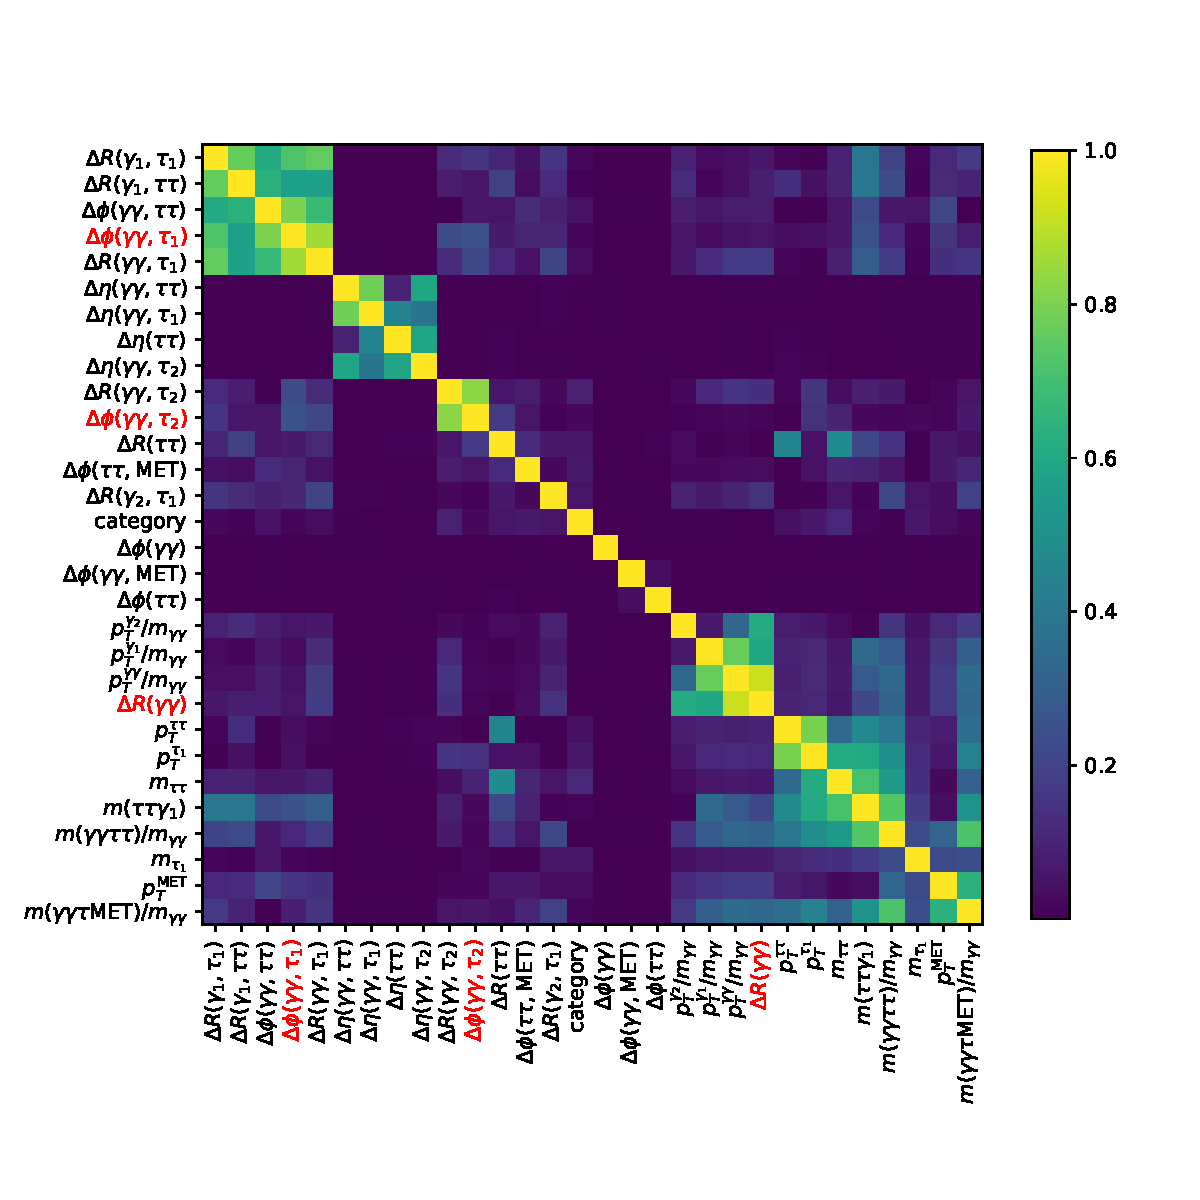
\includegraphics[width=\textwidth]{Figures/Dihiggs/categorisation/feature_correlation.pdf}
    \caption[Correlation Between the Most Important Training Features]{The Spearman rank correlation between the 31 features found after a selection procedure based on the feature importance from BDTs trained on the \XTwoHH signal samples. The dataset that the correlation is calculated in is a combination of the \XTwoHH ($\mX=300$\GeV) signal sample and the combined background sample. Only events which belong to categories with two tau lepton candidates are used so that are variables are well-defined, and for the same reason, $\pt^{j_1}$ is not shown since there is no guarantee that a jet is present in the event. The features highlighted in red are subsequently removed.}\label{fig:feature_correlation}
\end{figure}

When trialling features to remove, the impact on the efficiencies for the $\mX=260$, 300, 400, 500, 800 and 1000\GeV signal samples (including single tau lepton candidate category) was checked. After removing three features from the most correlated blocks of features, the greatest difference in signal efficiency was found to be 1\%, at which point the removal of features was stopped, leaving 28 selected features. These features, which are highlighted in red in \cref{fig:feature_correlation} are: $\dR(\gamma\gamma)$, $\dphi(\gamma\gamma,\tau_1)$ and $\dphi(\gamma\gamma, \tau_2)$. The changes in signal efficiencies for the different mass points are shown in \cref{tab:training_feature_subset_comparison}.

\begin{table}
    \centering
    \begin{tabular}{cccccc}
        \toprule
        \mX & AUC full & AUC subset & Sig.\ eff.\ full & Sig.\ eff.\ subset & Sig.\ eff.\ difference \\ \midrule
        260 & 0.9292 & 0.9279 & 48.43\% & 48.13\% & -0.30\% \\ 
        300 & 0.9513 & 0.9505 & 50.71\% & 51.77\% & -1.06\% \\ 
        400 & 0.9928 & 0.9926 & 86.05\% & 85.58\% & -0.47\% \\ 
        500 & 0.9980 & 0.9980 & 96.44\% & 96.48\% & +0.04\% \\ 
        800 & 0.9998 & 0.9998 & 99.85\% & 99.84\% & -0.01\% \\ 
        1000 & 0.9999 & 0.9999 & 99.95\% & 99.95\% & 0.00\% \\ \bottomrule
    \end{tabular}
    \caption[Performance Comparison Between Full Set of Training Features and Subset of Most Important Features]{Comparison of a BDT's performance to discriminate \XTwoHH signal samples from background when using the full set of 67 considered training features and when using the subset of 28 features found after the BDT feature importance procedure and the removal of three highly correlated features. The signal efficiencies are calculated at a background efficiency of 1\%.}\label{tab:training_feature_subset_comparison}
\end{table}

When training the pNNs with this selection of 28 features, sculpting of the \mgg distribution was found and this lead to the removal of $m(\gamma\gamma\tau_1 \MET) / \mgg$. For all but the high-mass \XYggHtt search, this was sufficient to eliminate any sculpting. In the high-mass \XYggHtt search, which has a significantly wider range in \mgg than the rest, it was found necessary to also remove $m(\ggtt) / \mgg$ and $m(\tau\tau\gamma_1)$. The final set of features used for training the pNNs is shown in \cref{tab:final_training_features}.

Distributions of the data and MC given the standard preselection (except for low-mass \Ygg) in all of the 27 final training features are given in \cref{fig:training_features_1,fig:training_features_2,fig:training_features_3,fig:training_features_4,fig:training_features_5,fig:training_features_6}. Also shown in these plots are signal distributions for the \XTwoHH process for $\mX=260$, 500 and 1000\GeV. For variables which are undefined in cases where there is a single tau candidate, e.g. $m_{\tau\tau}$, the single tau events are not included in the histograms. 

In general, better separation is seen for the $\mX = 1000$\GeV signal compared to 260\GeV. This is particularly apparent in variables such as $\pt^{\gamma\gamma}/\mgg$ (\cref{fig:training_features_1}), and $m(\ggtt) / \mgg$ (\cref{fig:training_features_6}), but there are also variables such as $\dR(\gamma_1, \tau_1)$ (\cref{fig:training_features_3}) which are more useful at lower \mX. This highlights the need for a selection of training features that considered the whole range of \mX.

The signal distributions of the \dR variables that represent the angular separation of the diphoton and ditau systems, or components thereof, e.g.\ $\dR(\gamma\gamma, \tau_1)$ in \cref{fig:training_features_2}, have shapes that might be difficult to understand initially. However, the shapes can be explained by separately considering the $\Delta\phi$ and $\Delta\eta$ components to \dR. At higher values of $\mX$, the Higgs bosons from the \XHH process are produced with higher \pt and approach the maximum separation in the $x-y$ plane that corresponds to $\Delta\phi=\pi$ (see $\Delta\phi(\gamma\gamma,\tau\tau$) in \cref{fig:training_features_3}). Consequently, the \dR variables peak at $\sim\pi$ and have a spread corresponding to the spread in $\Delta\eta$ (see $\Delta\eta(\gamma\gamma,\tau_1)$ in \cref{fig:training_features_2}). At lower values of \mX, e.g.\ $\mX=260$\GeV, there is less separation in the $x-y$ plane and therefore, the \dR variables spread towards lower values, and still retain a ``soft'' maximum at $\sim\pi$ due to the $\Delta\phi$ component.

\begin{table}
    \renewcommand{\arraystretch}{1.2}
    \centering
    \begin{tabular}{|c|c|}
    \toprule
        Photons & $\pt^{\gamma\gamma}/\mgg$, $\pt^{\gamma_1}/\mgg$, $\pt^{\gamma_2}/\mgg$, $\dR(\gamma\gamma)$, $\dphi(\gamma\gamma)$ \\ \midrule
        Tau candidates & $\pt^{\tau_1}, m(\tau_1), \pt^{\tau\tau}, m(\tau\tau), \dR(\tau\tau)$, $\deta(\tau\tau)$, $\dphi(\tau\tau)$ \\ \midrule
        Reconstructed \mX & ${m(\ggtt) / \mgg}^*$ \\ \midrule
        Additional angular & $\dphi(\gamma\gamma, \MET)$, $\dphi(\tau\tau, \MET)$, \\
        variables & $\Delta[\eta, R](\gamma\gamma,\tau_1)$, $\Delta[\eta, R](\gamma\gamma, \tau_2)$, \\
        & $\dphi(\gamma\gamma, \tau\tau)$, $\deta(\gamma\gamma, \tau\tau)$, \\
        & $\dR(\gamma_1, \tau\tau)$, $\dR(\gamma_1, \tau_1)$, $\dR(\gamma_2, \tau_1)$ \\ \midrule
        Other & ${m(\tau\tau\gamma_1)}^*$, $\pt^{\MET}$, $\pt^{j_1}$, category \\ \bottomrule
    \end{tabular}
    \caption[Final pNN Training Features]{The 27 final features selected to train the pNNs determined by a feature importance procedure, removing highly correlated variables, and removing variables which lead to sculpting of the \mgg distribution. The features, $m(\ggtt) / \mgg$ and $m(\tau\tau\gamma_1)$, are marked with an asterisk to indicate that they are not used in the high-mass \XYggHtt search. Leading and subleading particles are denoted by $p_1$ and $p_2$ respectively. The $[x,y,z]$ notation means there is a variable for each choice in $[x,y,z]$, e.g.\ $\dall(\gamma\gamma, \tau_1)$ corresponds to $\deta(\gamma\gamma, \tau_1), \dphi(\gamma\gamma, \tau_1), \dR(\gamma\gamma, \tau_1)$.}\label{tab:final_training_features}
\end{table}

\begin{table}
    \centering
    \begin{tabular}{c|c}
        Channel Number & Tau candidates \\
        \midrule
        1 & $\tauh\mu$ \\
        2 & $\tauh e$ \\
        3 & $\tauh\tauh$ \\
        4 & $\mu\mu$ \\
        5 & $ee$ \\
        6 & $\mu e$ \\
        7 & $\tauh + \text{IsoTrack}$ \\
        8 & $\tauh$ \\
    \end{tabular}
    \caption[Numbering Scheme Used to Describe the Channels in the Di-Higgs Analysis]{Numbering scheme used to describe the channels in the analysis which differ based upon the types and number of tau lepton candidates reconstructed.}\label{tab:channel}
\end{table}

\begin{figure}
    \centering
    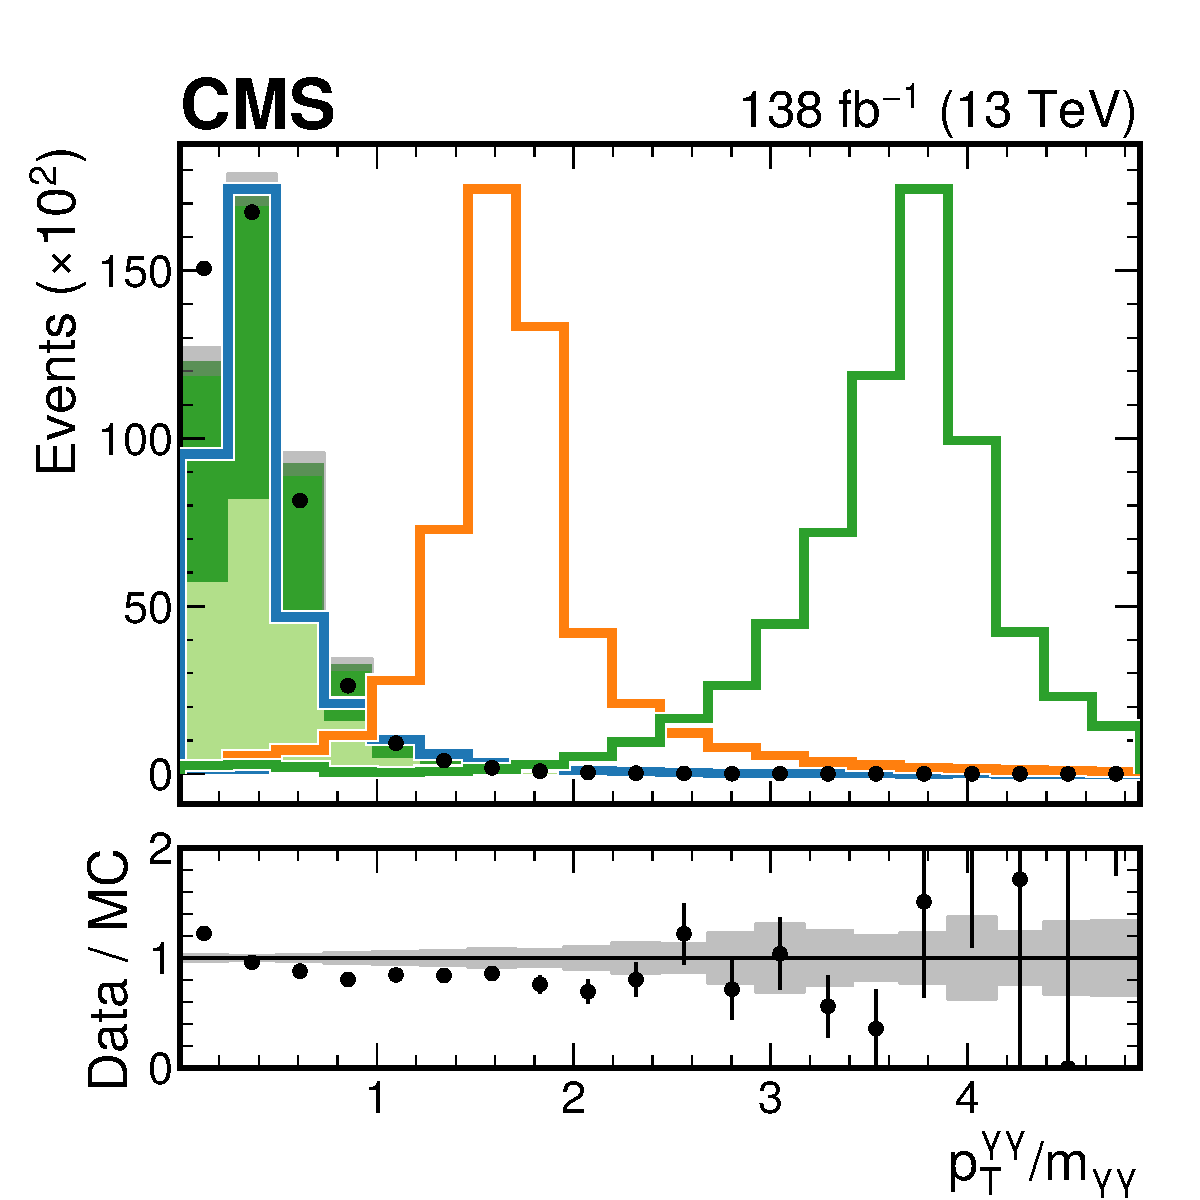
\includegraphics[width=.49\linewidth]{Figures/Dihiggs/categorisation/input_features/Graviton/Scale_equal/Diphoton_pt_mgg_GluGluToBulkGravitonToHHTo2G2Tau_M-1000_linear.pdf}
    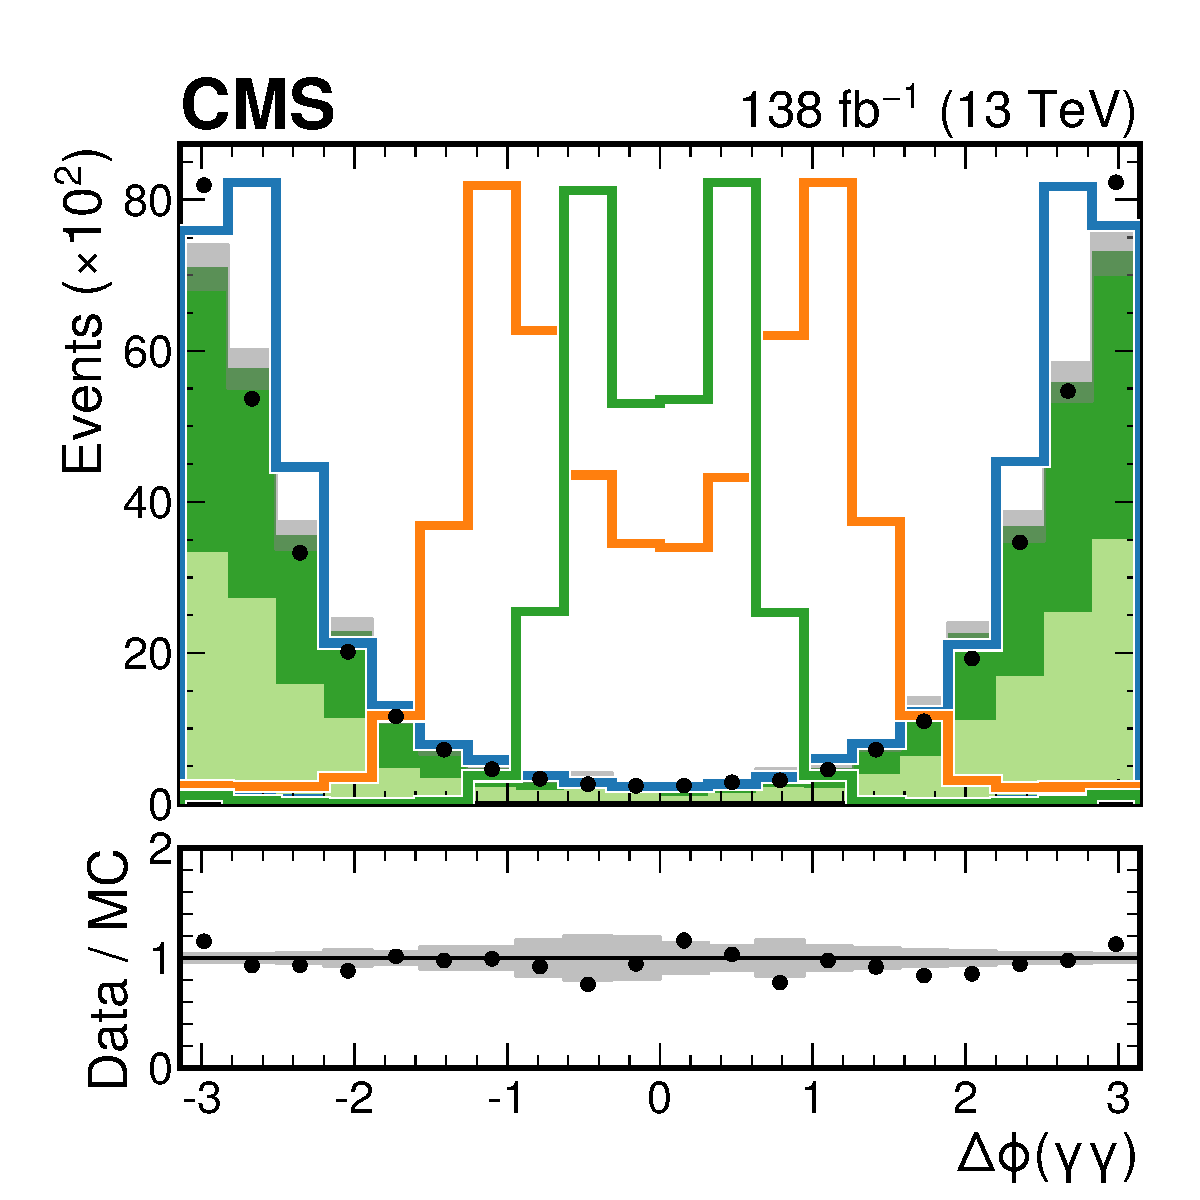
\includegraphics[width=.49\linewidth]{Figures/Dihiggs/categorisation/input_features/Graviton/Scale_equal/Diphoton_dPhi_GluGluToBulkGravitonToHHTo2G2Tau_M-1000_linear.pdf} \\
    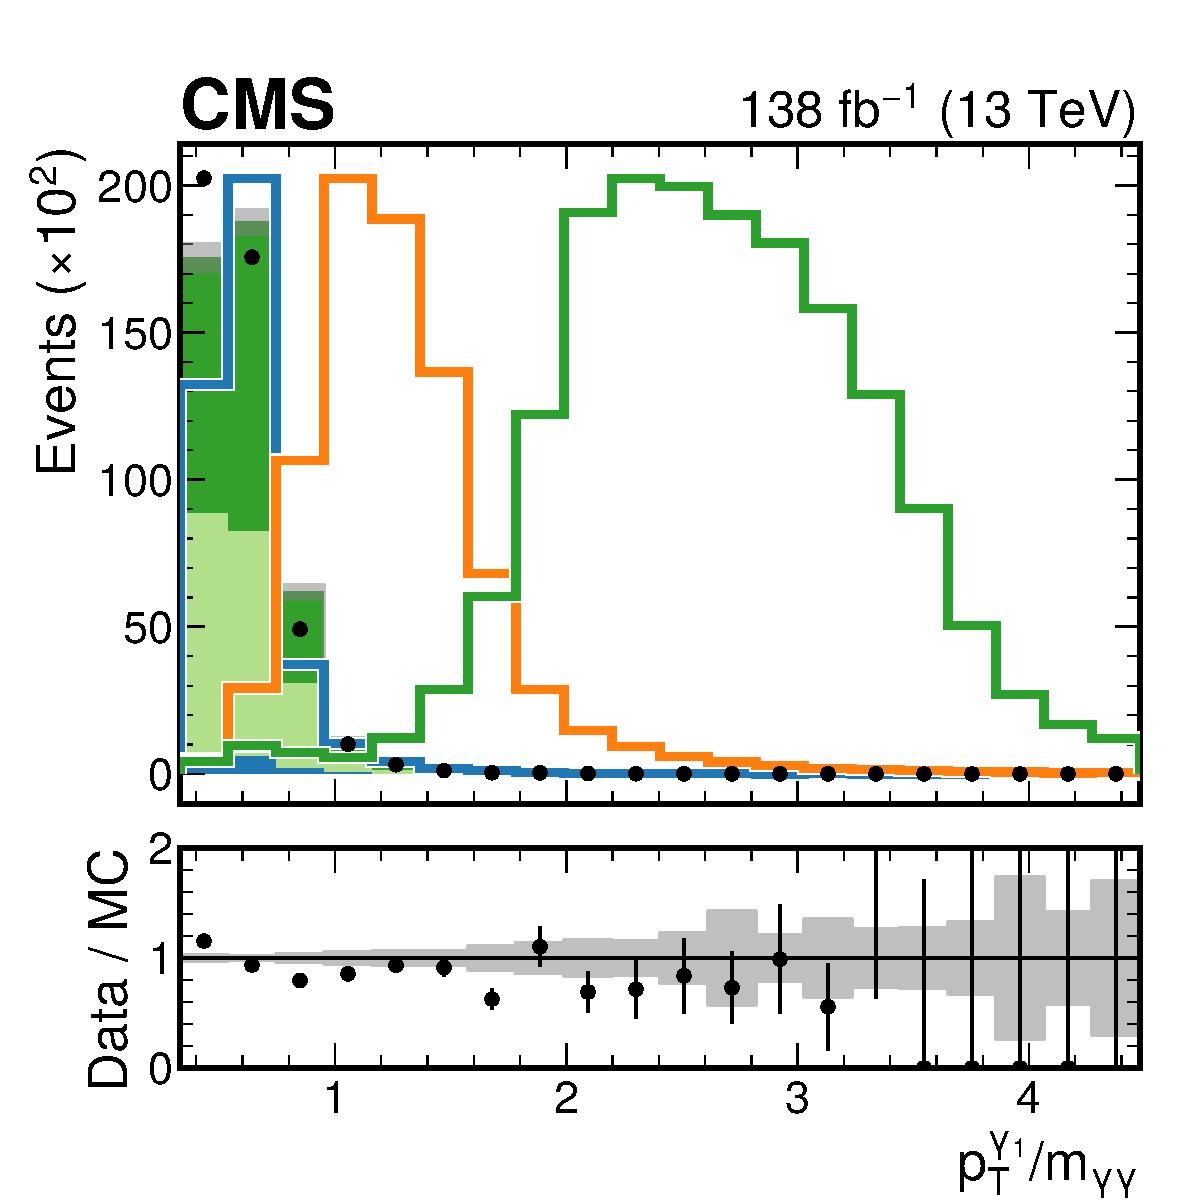
\includegraphics[width=.49\linewidth]{Figures/Dihiggs/categorisation/input_features/Graviton/Scale_equal/LeadPhoton_pt_mgg_GluGluToBulkGravitonToHHTo2G2Tau_M-1000_linear.pdf}
    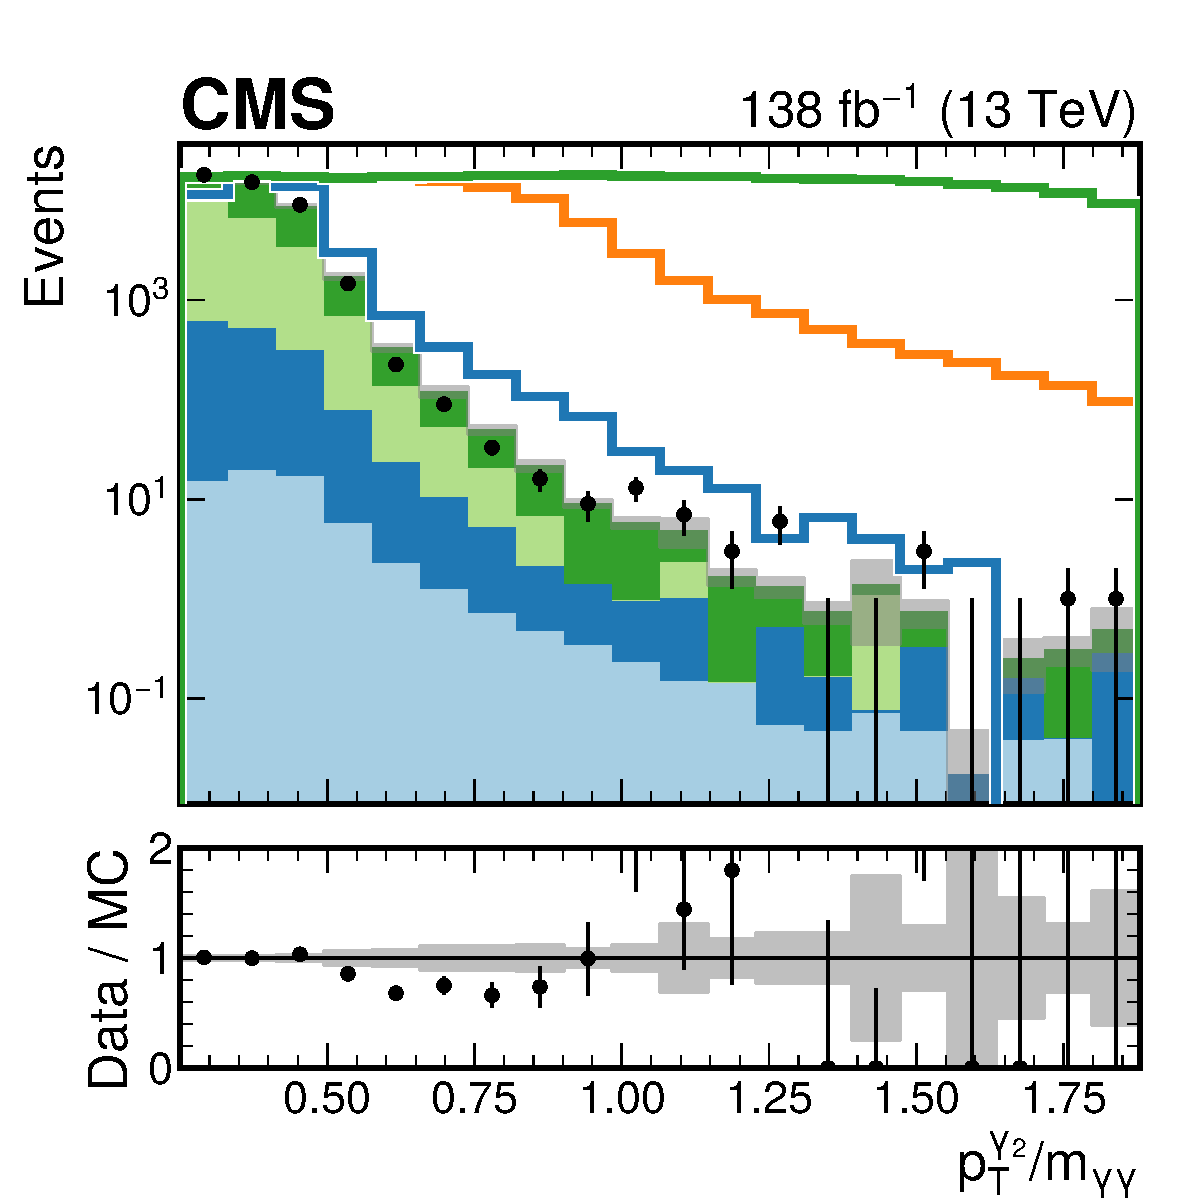
\includegraphics[width=.49\linewidth]{Figures/Dihiggs/categorisation/input_features/Graviton/Scale_equal/SubleadPhoton_pt_mgg_GluGluToBulkGravitonToHHTo2G2Tau_M-1000_log.pdf} \\
    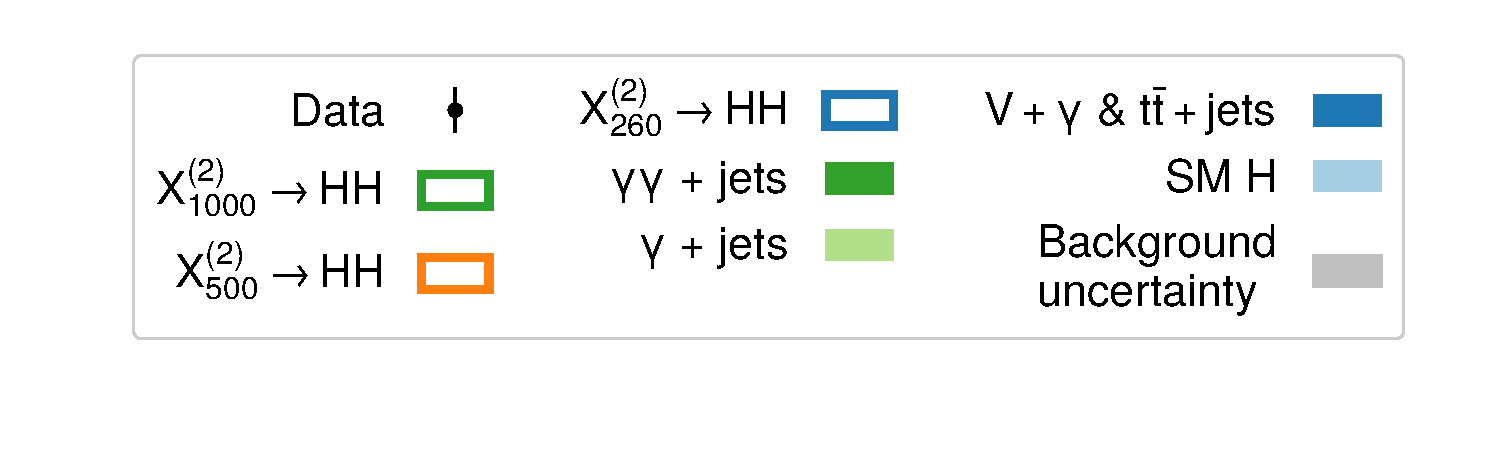
\includegraphics[width=.7\linewidth]{Figures/Dihiggs/categorisation/input_features/Graviton/Scale_equal/legend.pdf}
    \caption[Distributions of Training Features (1)]{Distributions of data, background MC, and \XTwoHH signals for $\mX=260$, 700 and 1000\GeV, in a subset of the variables used to train the pNN. Background MC is normalized to data and the signal's normalization is arbitrary. The statistical uncertainty in the background simulation is shown by the grey shaded bands.}\label{fig:training_features_1}
\end{figure}

\begin{figure}
    \centering
    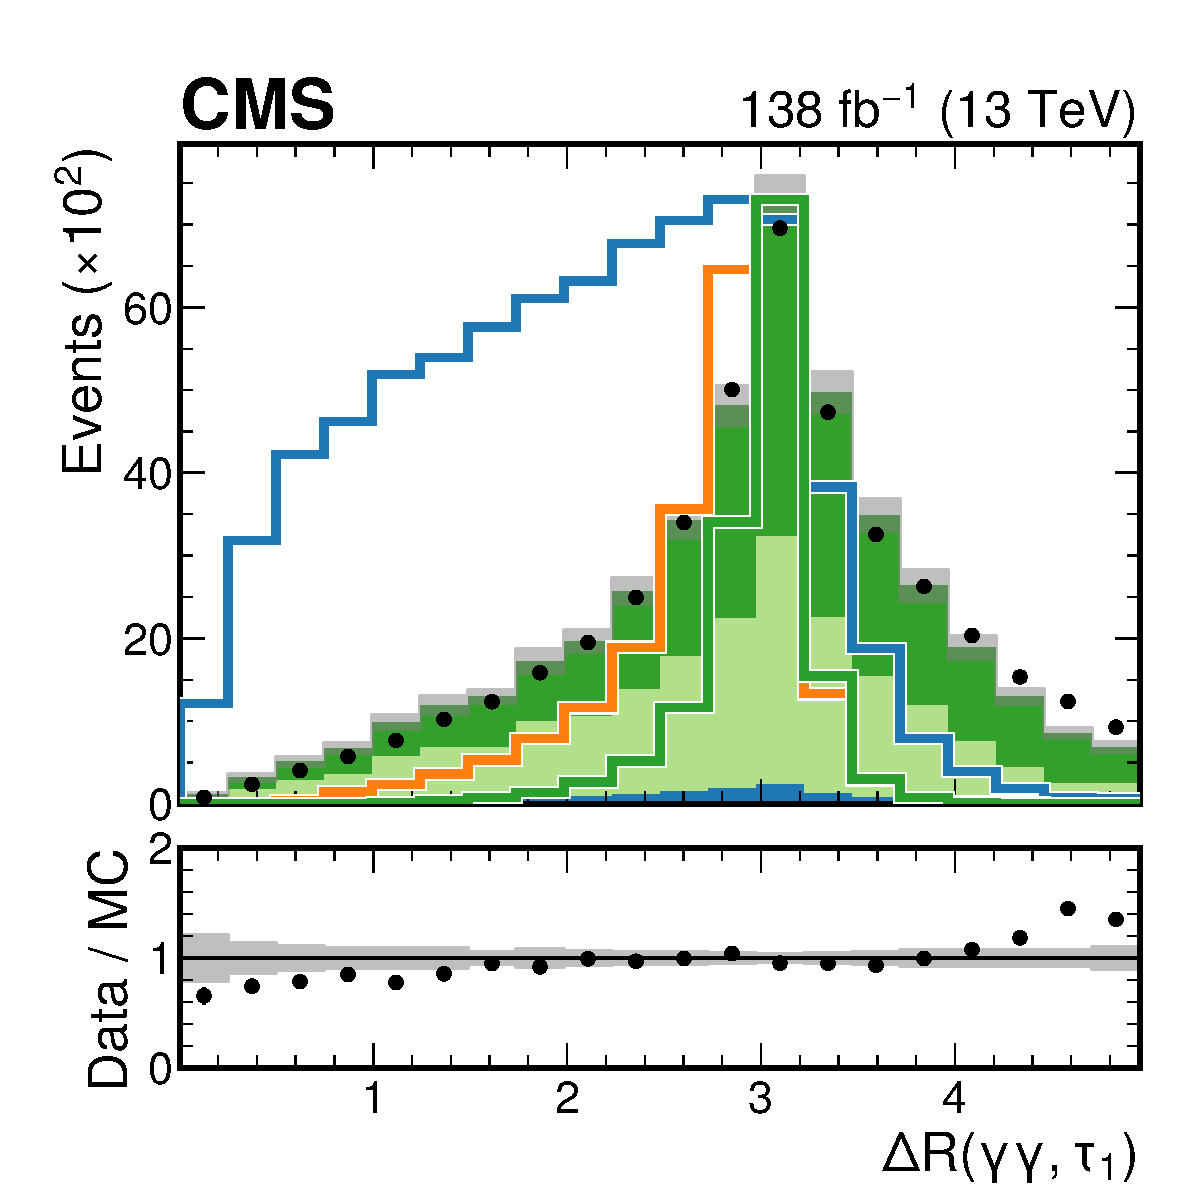
\includegraphics[width=.49\linewidth]{Figures/Dihiggs/categorisation/input_features/Graviton/Scale_equal/Diphoton_lead_lepton_dR_GluGluToBulkGravitonToHHTo2G2Tau_M-1000_linear.pdf}
    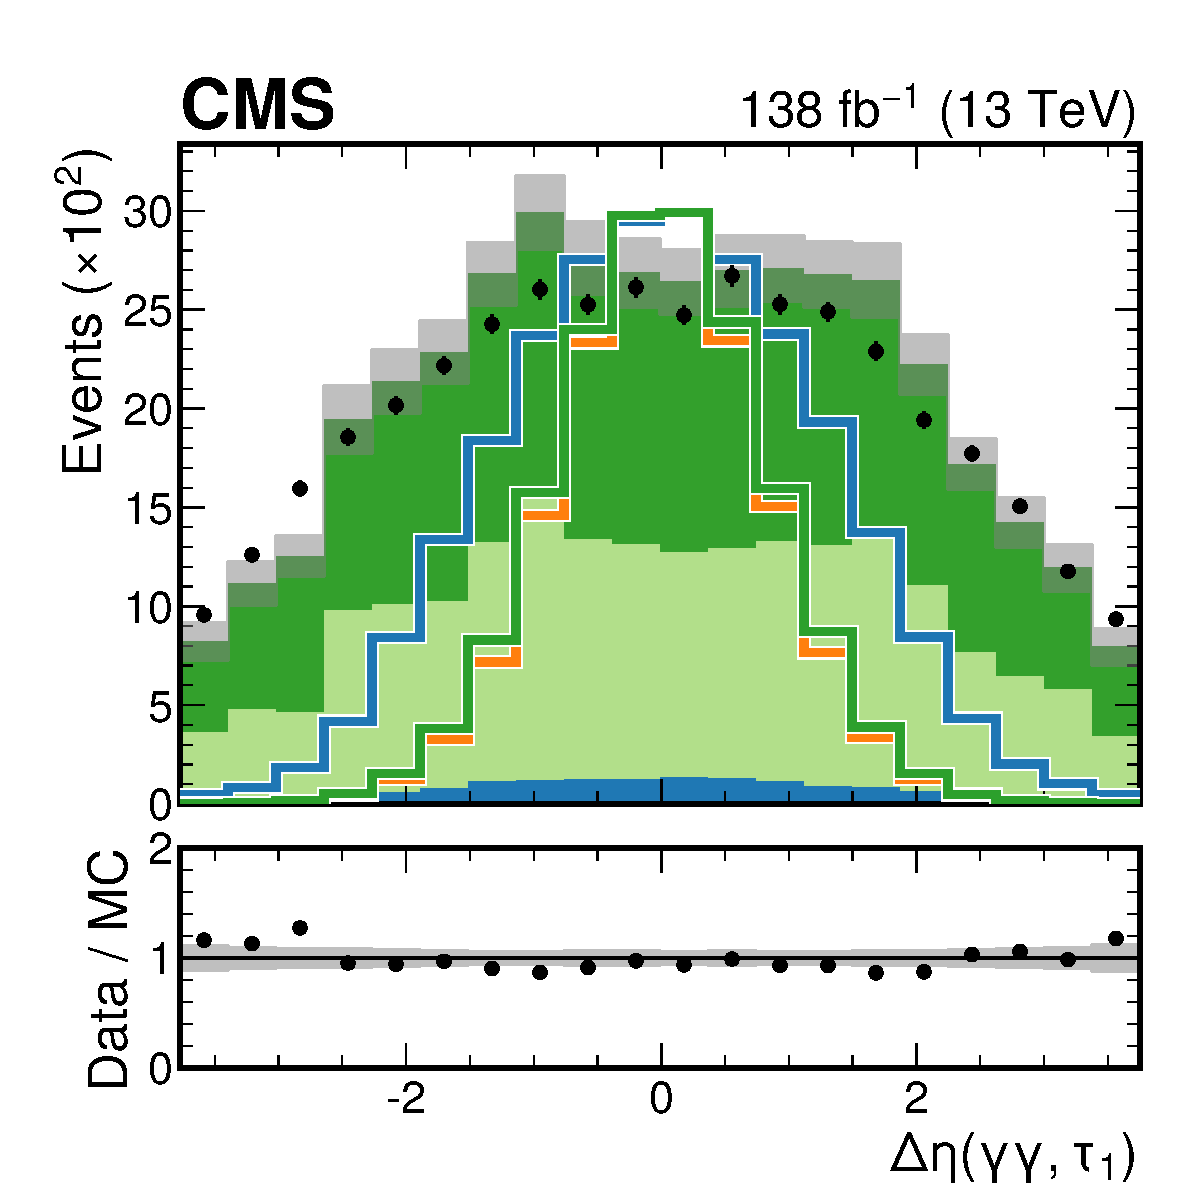
\includegraphics[width=.49\linewidth]{Figures/Dihiggs/categorisation/input_features/Graviton/Scale_equal/Diphoton_lead_lepton_deta_GluGluToBulkGravitonToHHTo2G2Tau_M-1000_linear.pdf} \\
    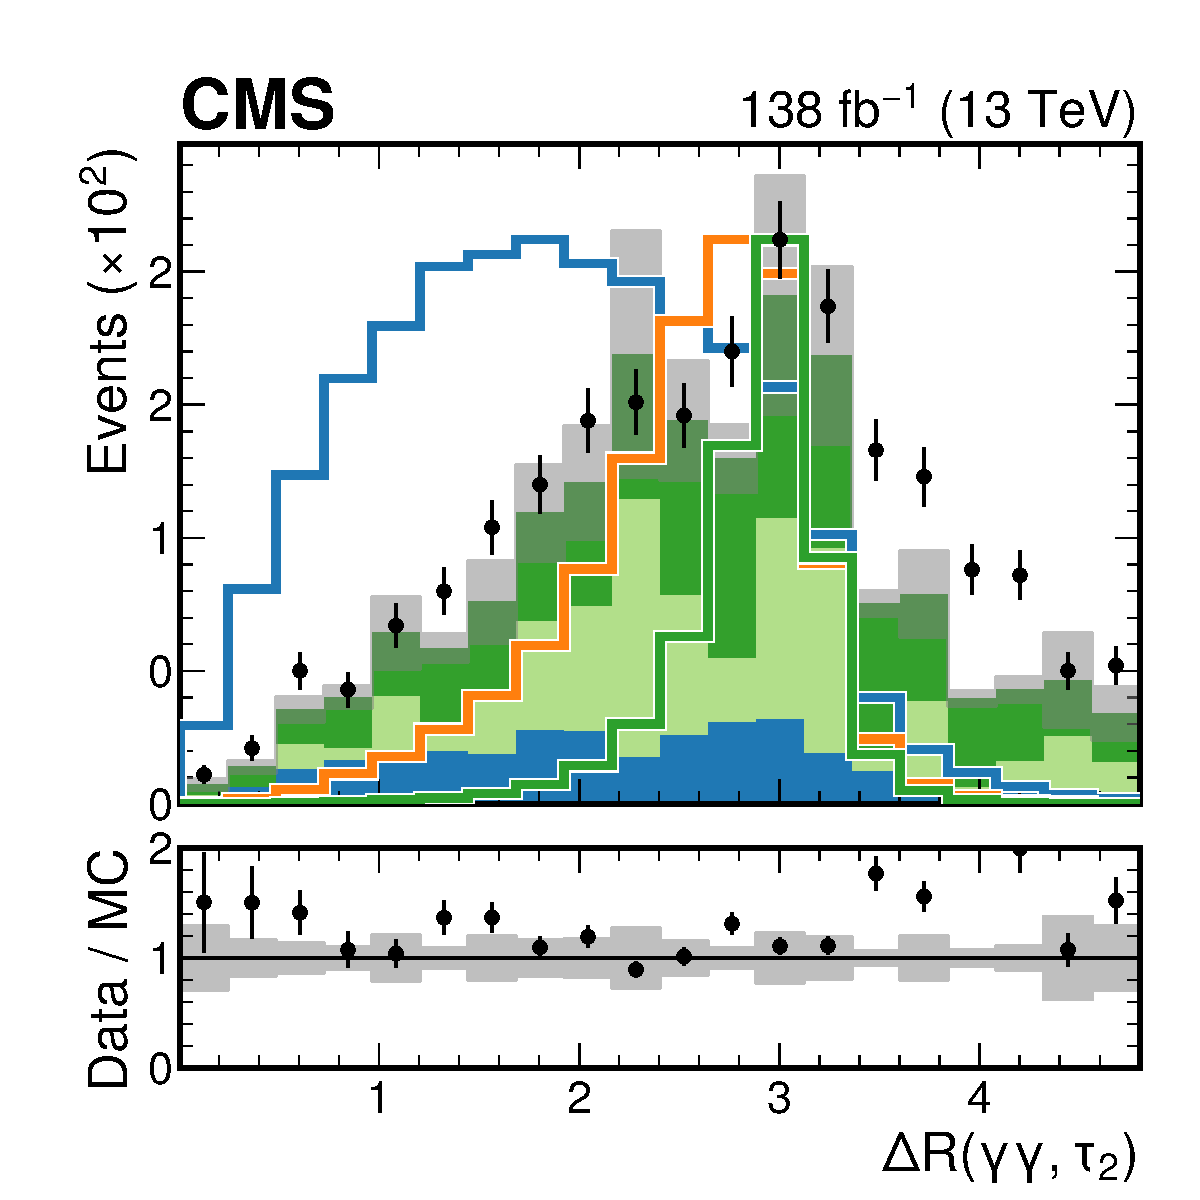
\includegraphics[width=.49\linewidth]{Figures/Dihiggs/categorisation/input_features/Graviton/Scale_equal/Diphoton_sublead_lepton_dR_GluGluToBulkGravitonToHHTo2G2Tau_M-1000_linear.pdf} 
    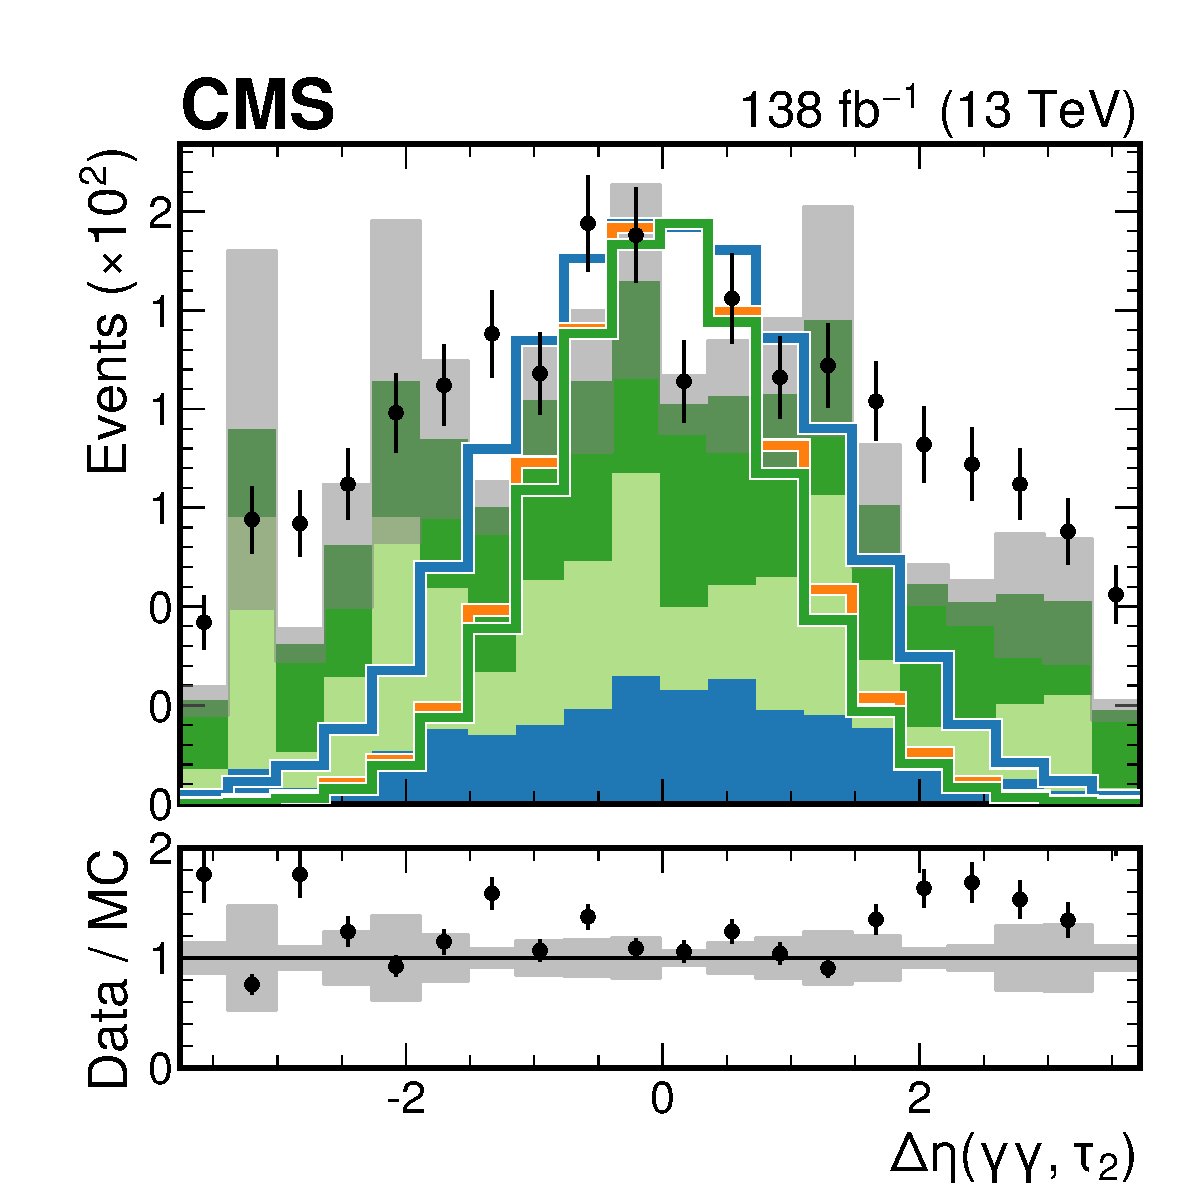
\includegraphics[width=.49\linewidth]{Figures/Dihiggs/categorisation/input_features/Graviton/Scale_equal/Diphoton_sublead_lepton_deta_GluGluToBulkGravitonToHHTo2G2Tau_M-1000_linear.pdf}
    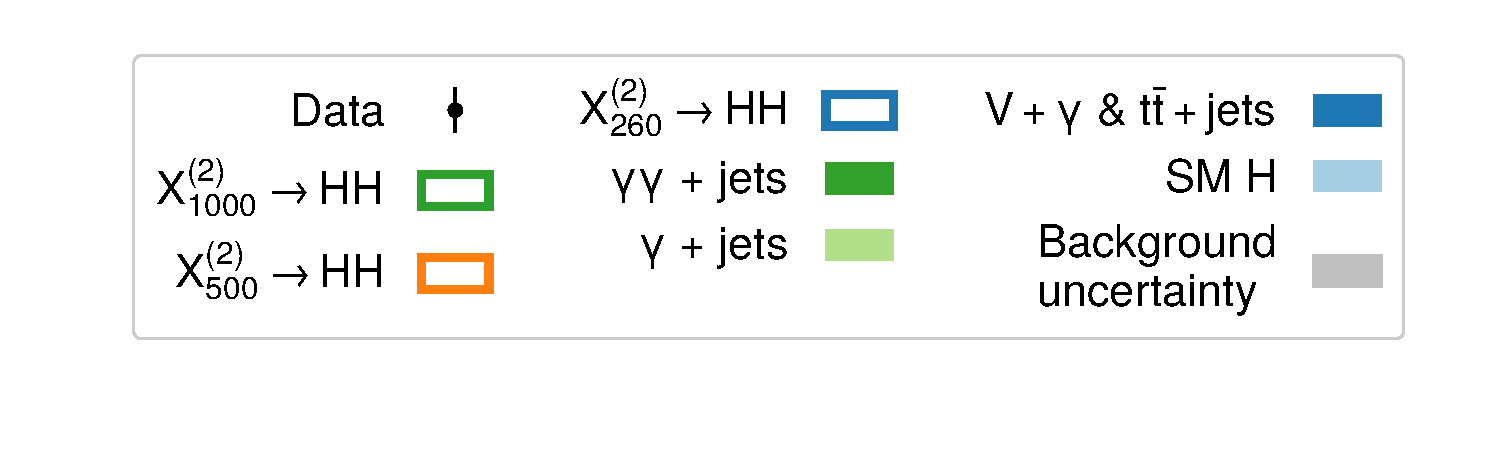
\includegraphics[width=.7\linewidth]{Figures/Dihiggs/categorisation/input_features/Graviton/Scale_equal/legend.pdf}
    \caption[Distributions of Training Features (2)]{Distributions of data, background MC, and \XTwoHH signals for $\mX=260$, 700 and 1000\GeV, in a subset of the variables used to train the pNN. Background MC is normalized to data and the signal's normalization is arbitrary. The statistical uncertainty in the background simulation is shown by the grey shaded bands.}\label{fig:training_features_2}
\end{figure}

\begin{figure}
    \centering
    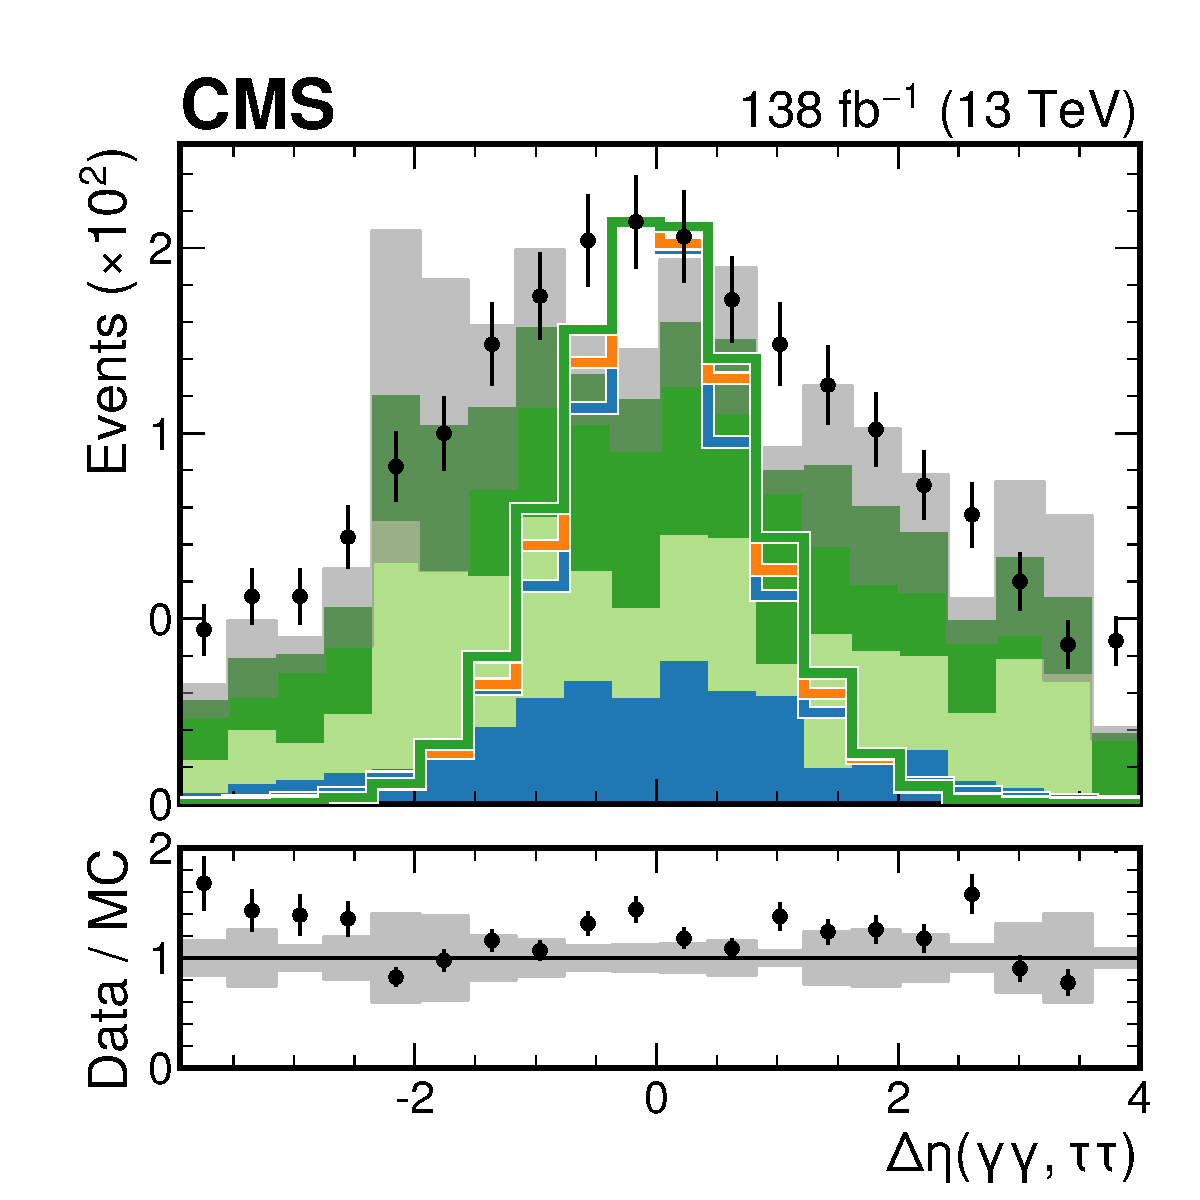
\includegraphics[width=.49\linewidth]{Figures/Dihiggs/categorisation/input_features/Graviton/Scale_equal/Diphoton_ditau_deta_GluGluToBulkGravitonToHHTo2G2Tau_M-1000_linear.pdf}
    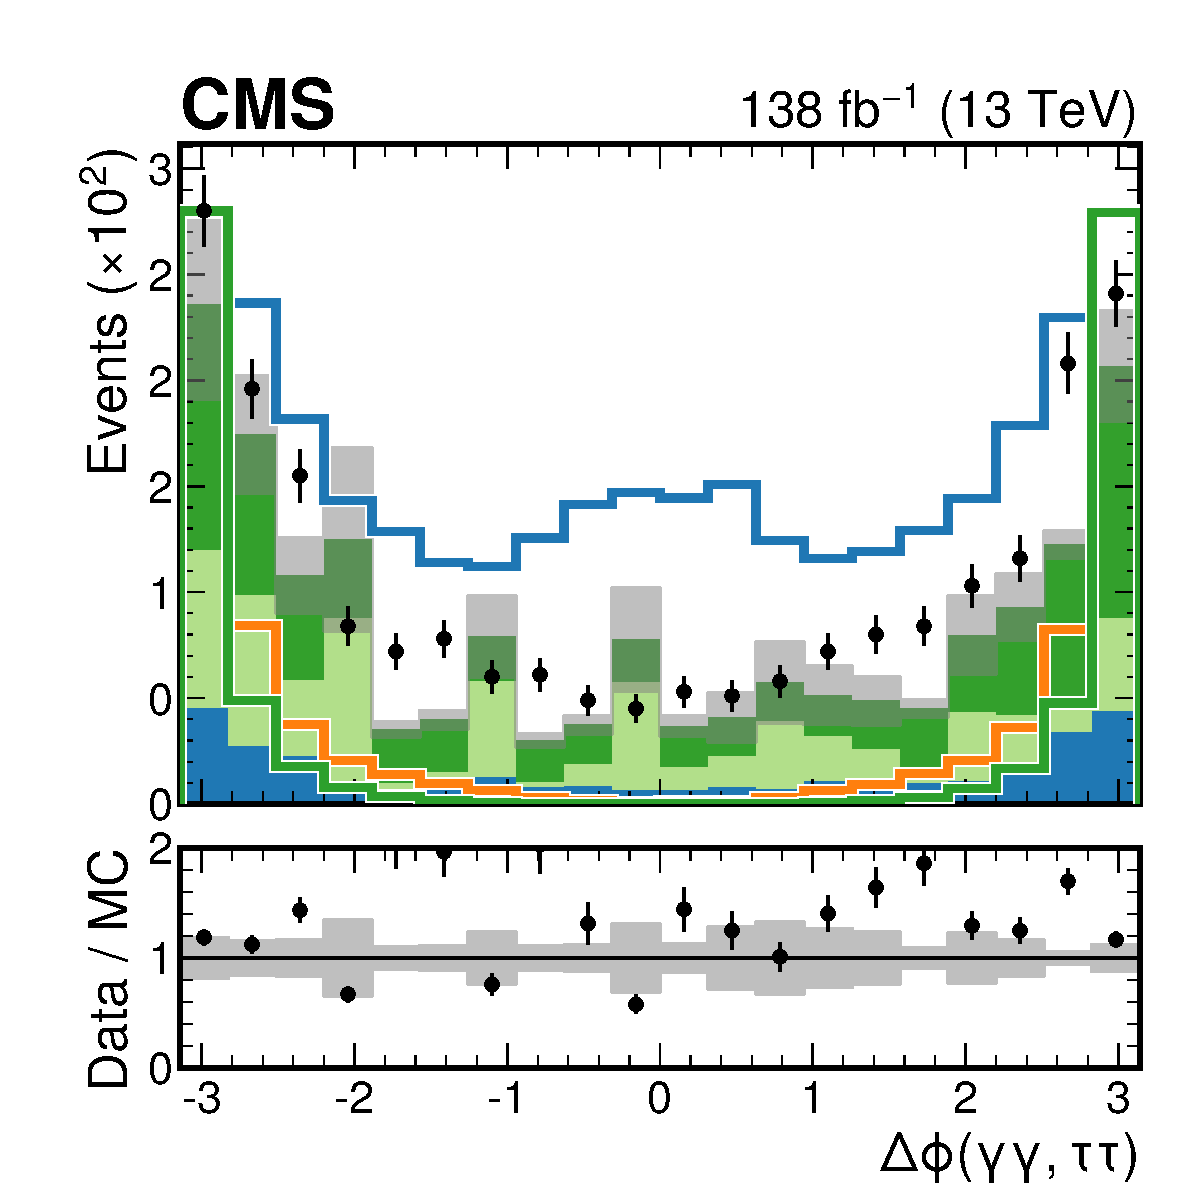
\includegraphics[width=.49\linewidth]{Figures/Dihiggs/categorisation/input_features/Graviton/Scale_equal/Diphoton_ditau_dphi_GluGluToBulkGravitonToHHTo2G2Tau_M-1000_linear.pdf} \\
    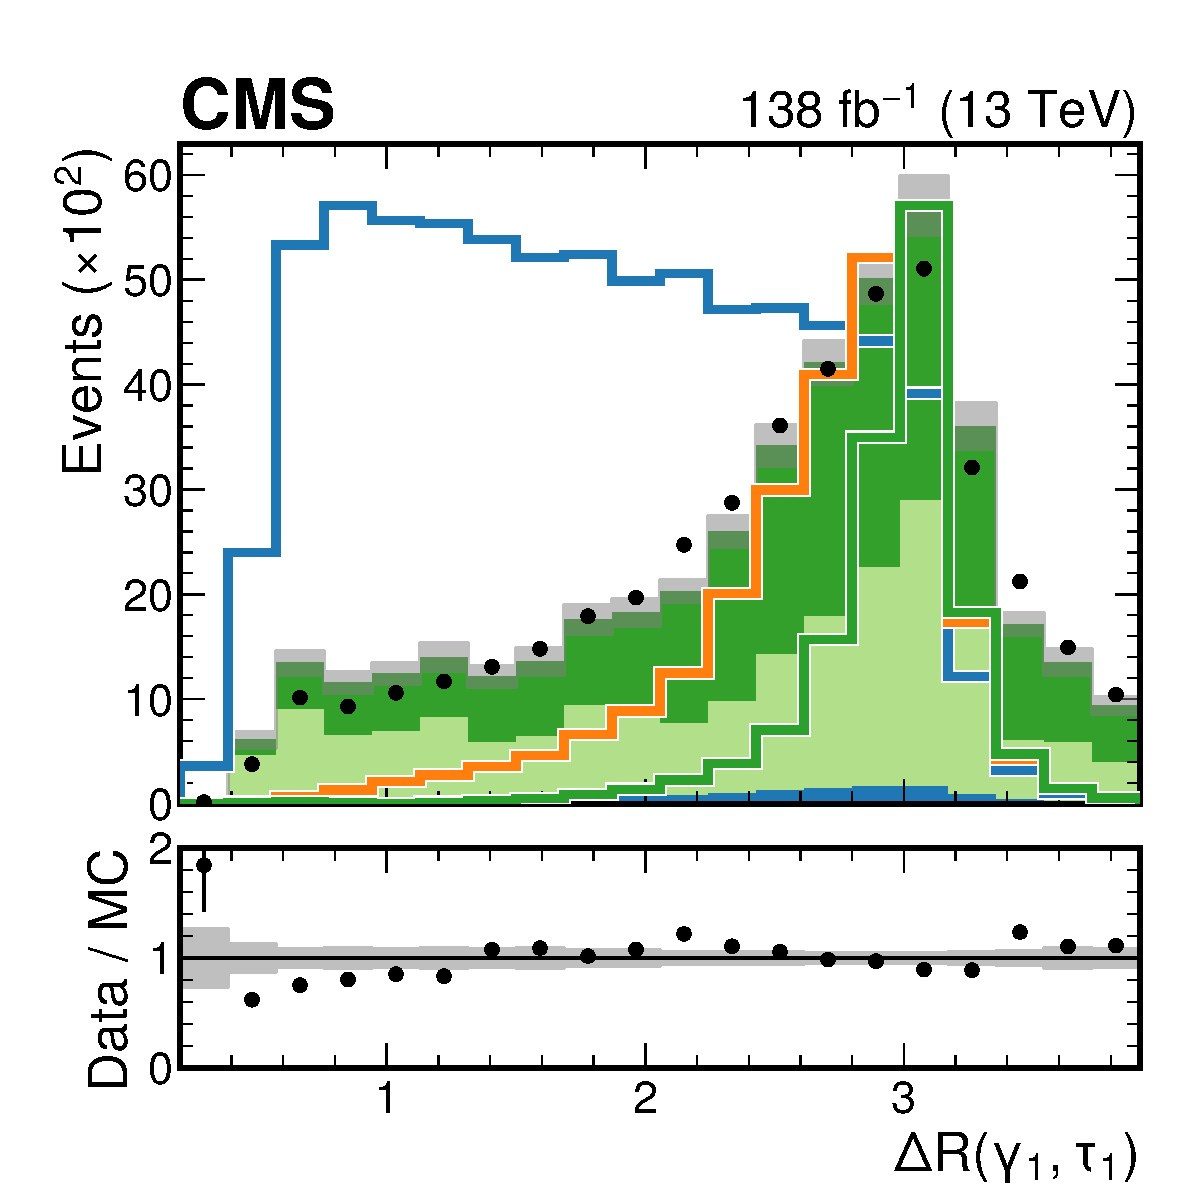
\includegraphics[width=.49\linewidth]{Figures/Dihiggs/categorisation/input_features/Graviton/Scale_equal/LeadPhoton_lead_lepton_dR_GluGluToBulkGravitonToHHTo2G2Tau_M-1000_linear.pdf}
    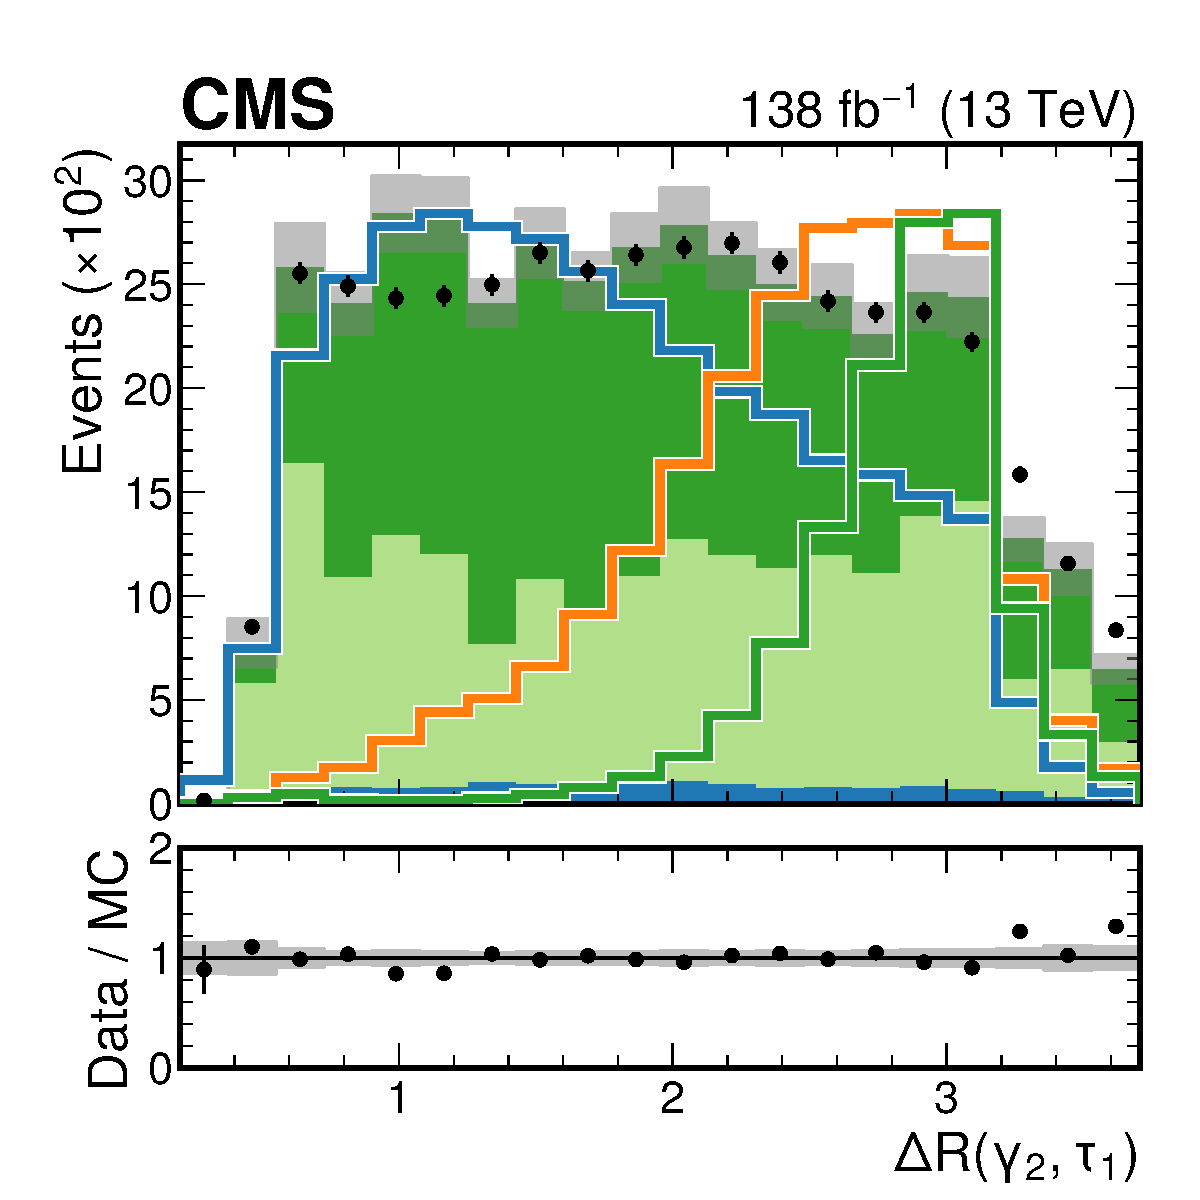
\includegraphics[width=.49\linewidth]{Figures/Dihiggs/categorisation/input_features/Graviton/Scale_equal/SubleadPhoton_lead_lepton_dR_GluGluToBulkGravitonToHHTo2G2Tau_M-1000_linear.pdf} \\
    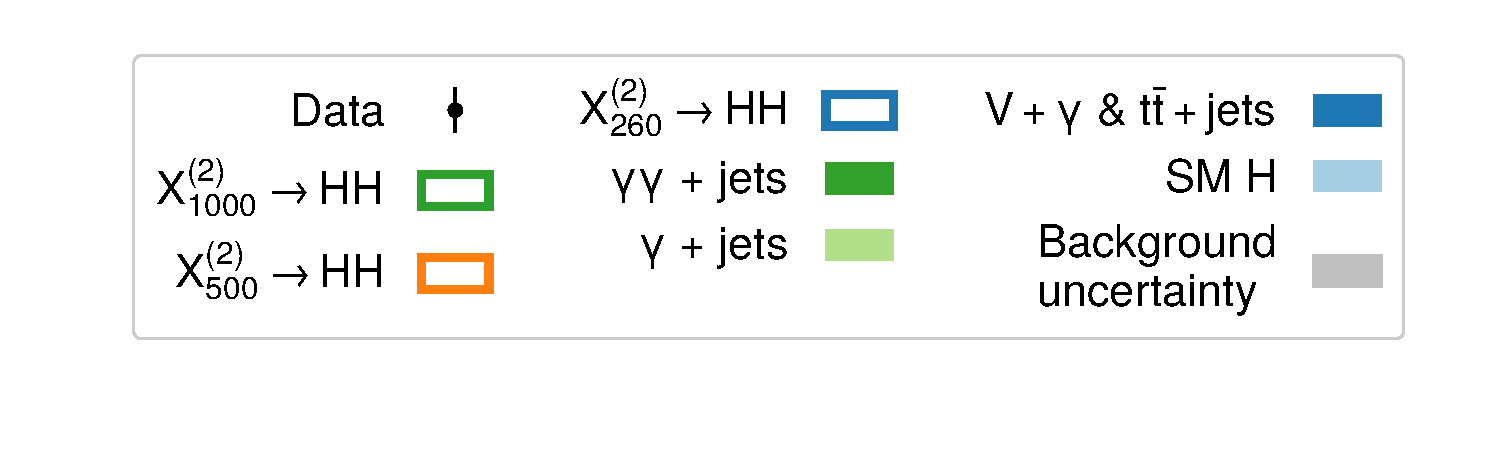
\includegraphics[width=.7\linewidth]{Figures/Dihiggs/categorisation/input_features/Graviton/Scale_equal/legend.pdf}
    \caption[Distributions of Training Features (3)]{Distributions of data, background MC, and \XTwoHH signals for $\mX=260$, 700 and 1000\GeV, in a subset of the variables used to train the pNN. Background MC is normalized to data and the signal's normalization is arbitrary. The statistical uncertainty in the background simulation is shown by the grey shaded bands.}\label{fig:training_features_3}
\end{figure}

\begin{figure}
    \centering
    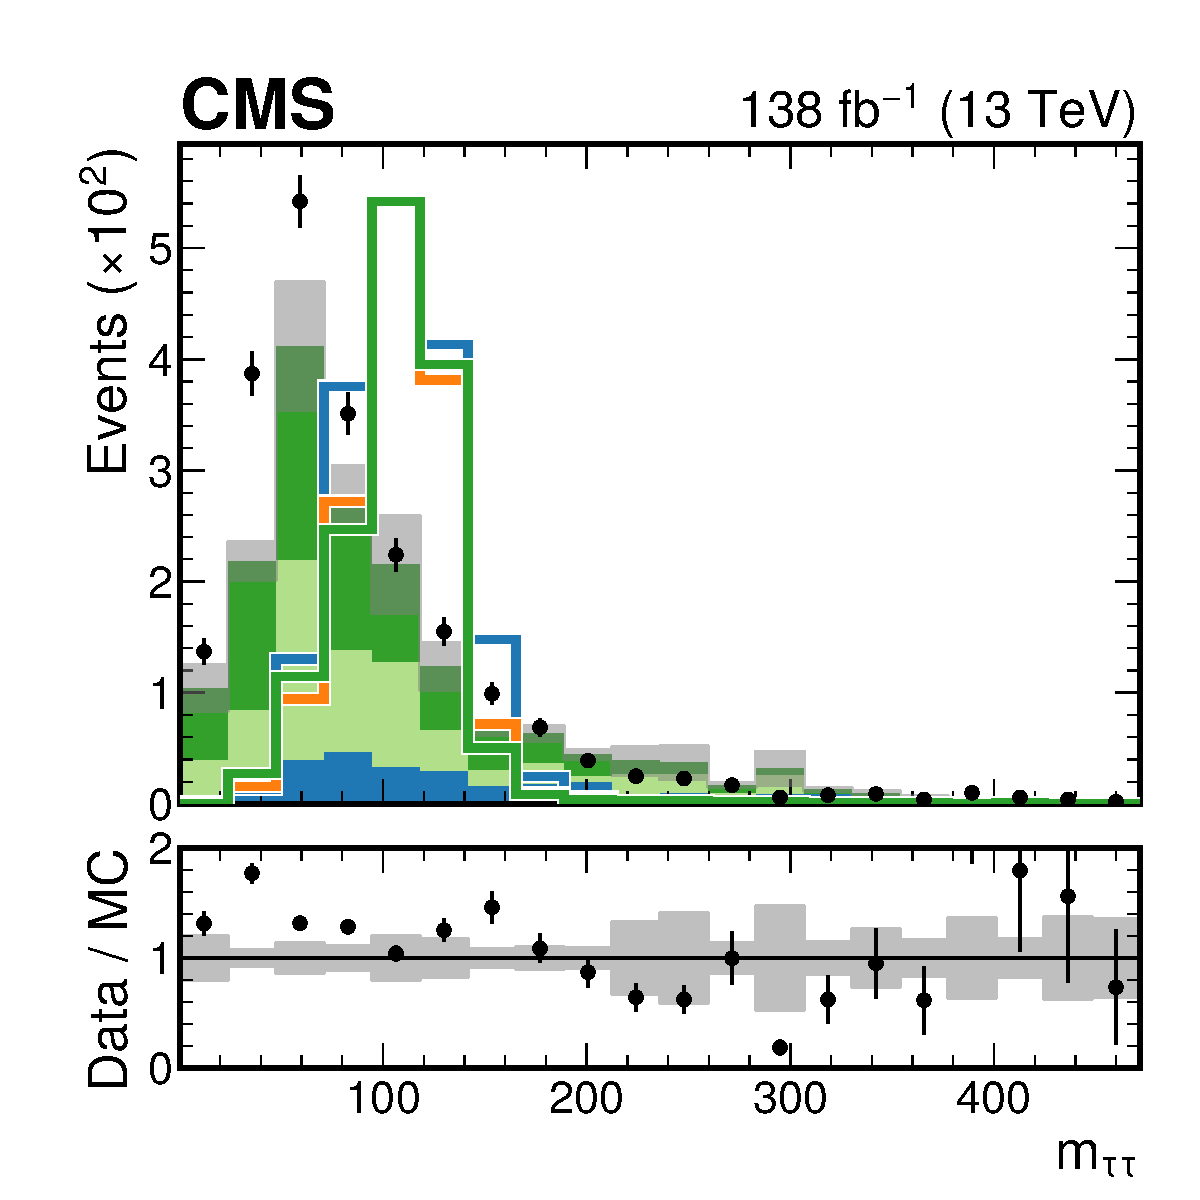
\includegraphics[width=.49\linewidth]{Figures/Dihiggs/categorisation/input_features/Graviton/Scale_equal/ditau_mass_GluGluToBulkGravitonToHHTo2G2Tau_M-1000_linear.pdf}
    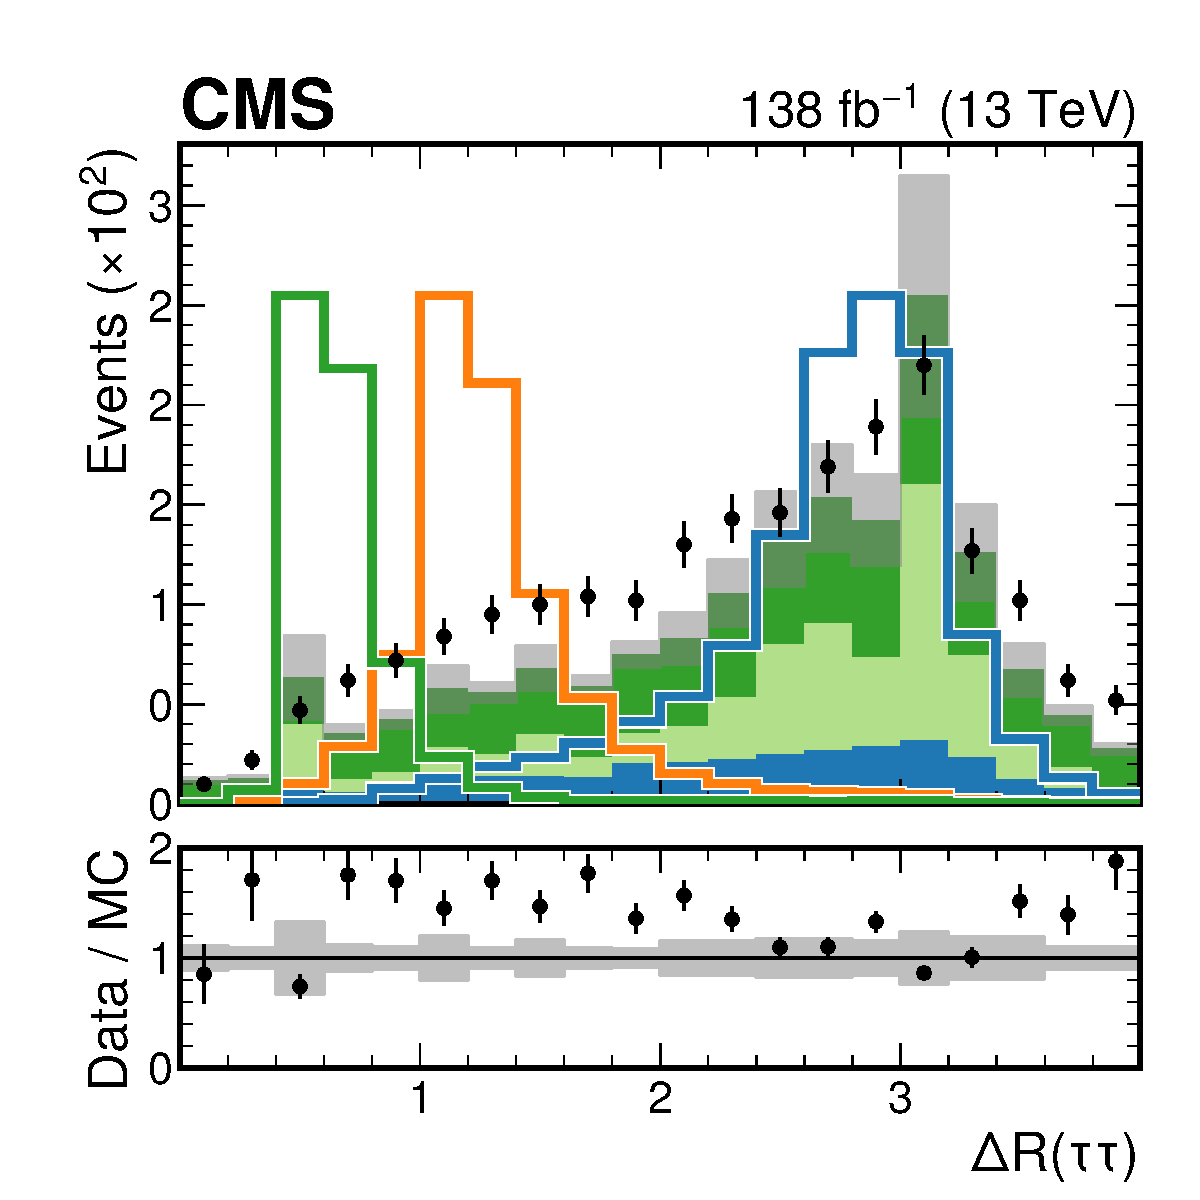
\includegraphics[width=.49\linewidth]{Figures/Dihiggs/categorisation/input_features/Graviton/Scale_equal/ditau_dR_GluGluToBulkGravitonToHHTo2G2Tau_M-1000_linear.pdf} \\
    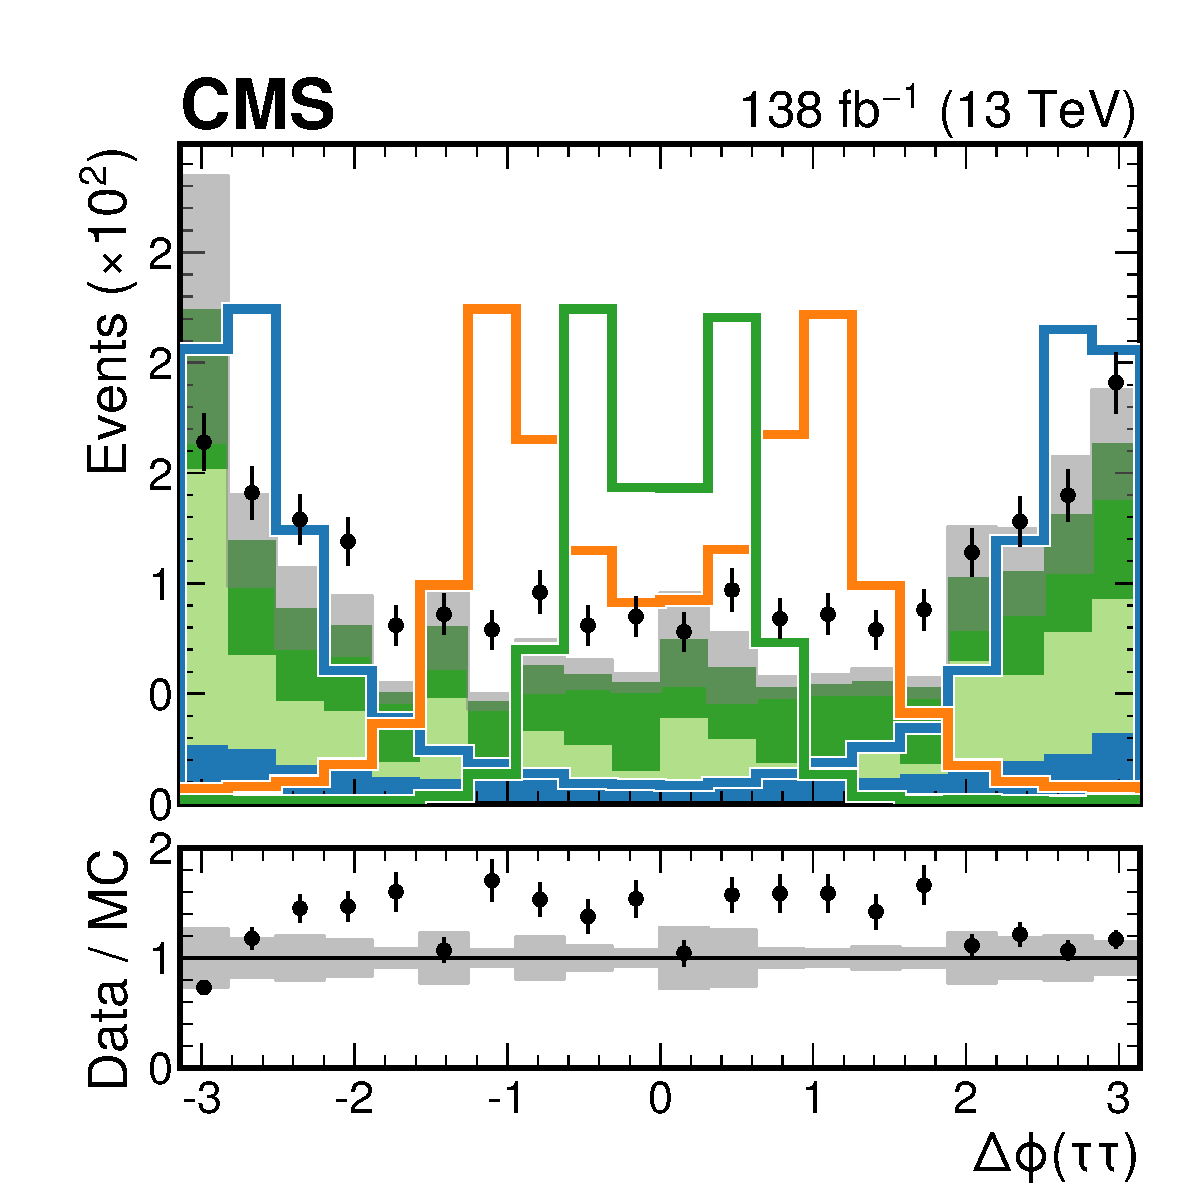
\includegraphics[width=.49\linewidth]{Figures/Dihiggs/categorisation/input_features/Graviton/Scale_equal/ditau_dphi_GluGluToBulkGravitonToHHTo2G2Tau_M-1000_linear.pdf}
    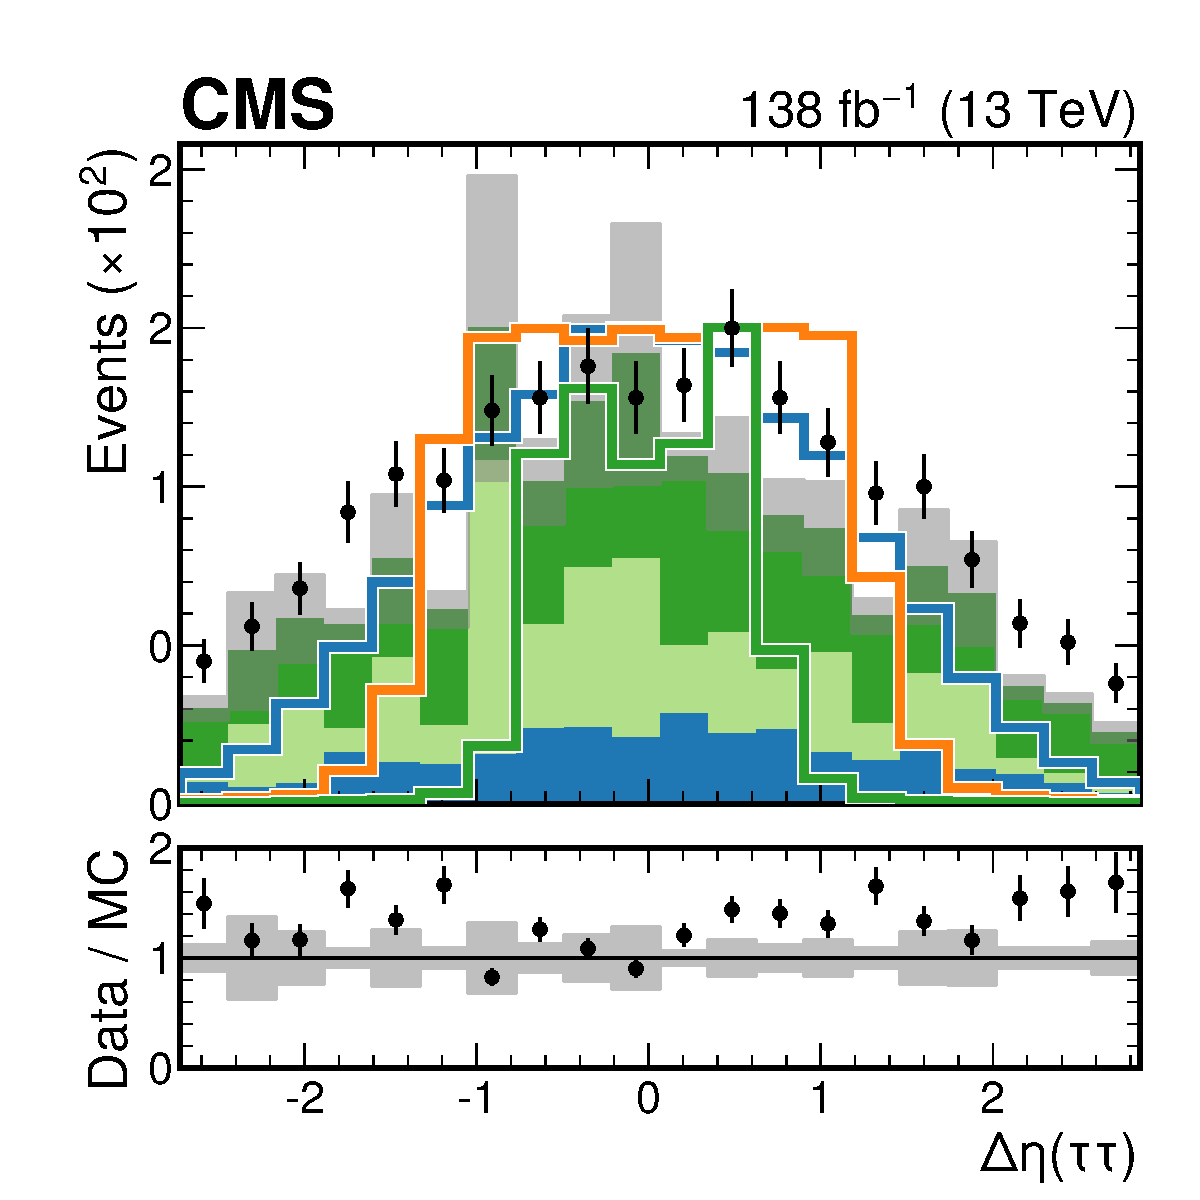
\includegraphics[width=.49\linewidth]{Figures/Dihiggs/categorisation/input_features/Graviton/Scale_equal/ditau_deta_GluGluToBulkGravitonToHHTo2G2Tau_M-1000_linear.pdf} \\
    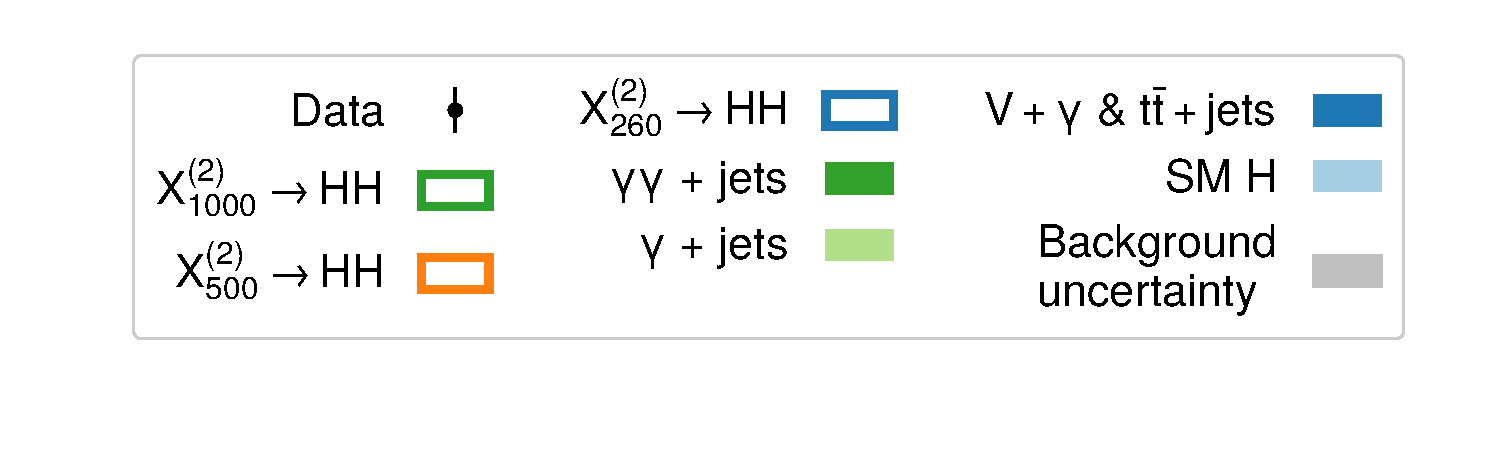
\includegraphics[width=.7\linewidth]{Figures/Dihiggs/categorisation/input_features/Graviton/Scale_equal/legend.pdf}
    \caption[Distributions of Training Features (4)]{Distributions of data, background MC, and \XTwoHH signals for $\mX=260$, 700 and 1000\GeV, in a subset of the variables used to train the pNN. Background MC is normalized to data and the signal's normalization is arbitrary. The statistical uncertainty in the background simulation is shown by the grey shaded bands.}\label{fig:training_features_4}
\end{figure}

\begin{figure}
    \centering
    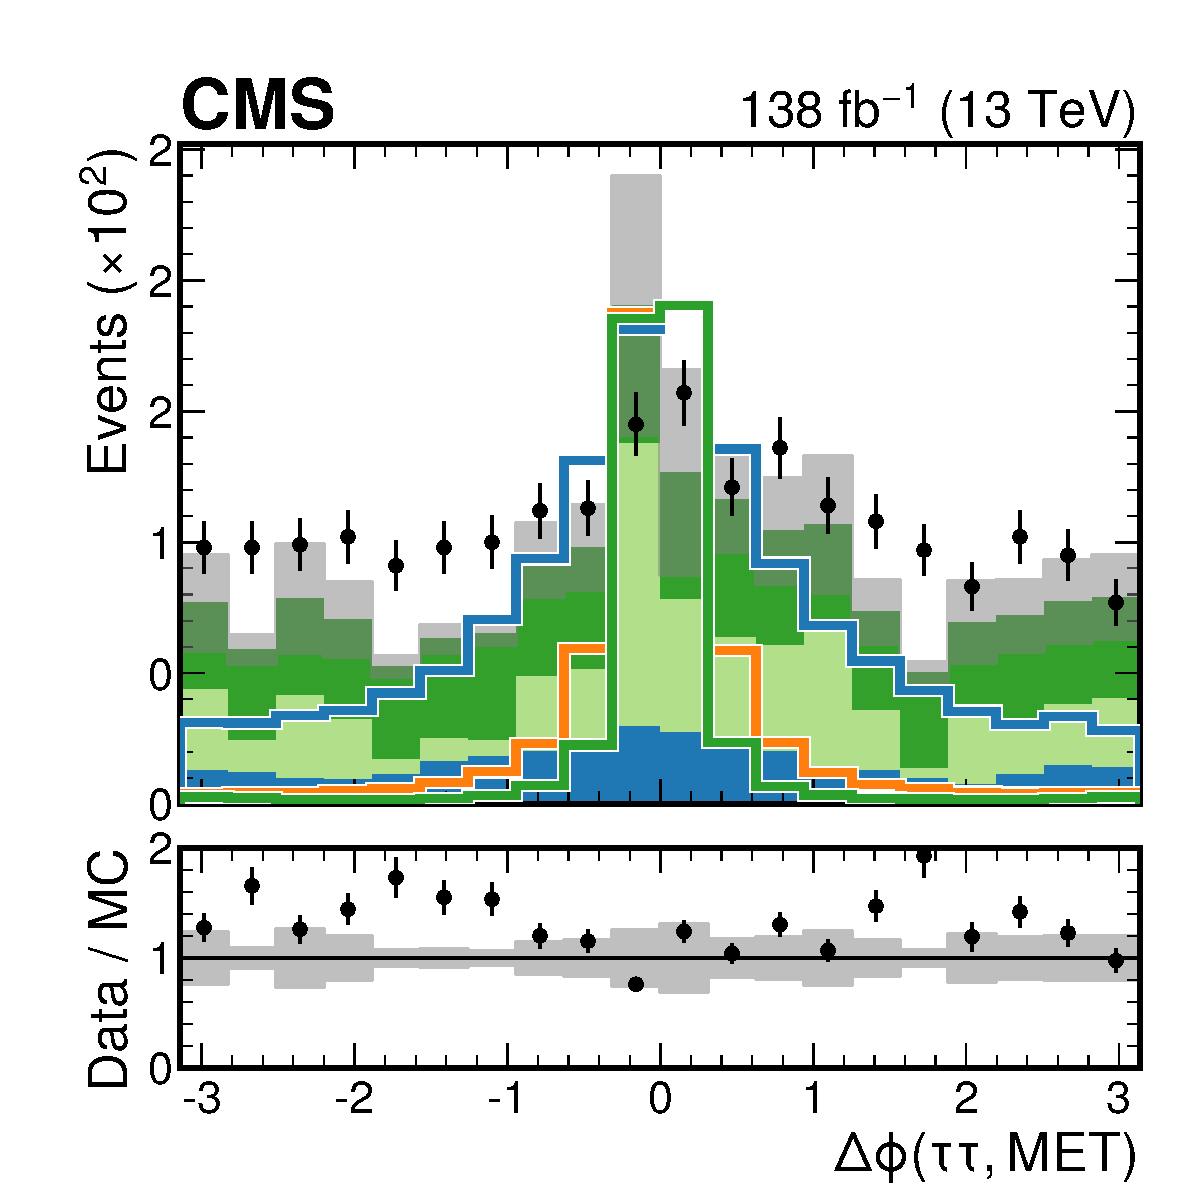
\includegraphics[width=.49\linewidth]{Figures/Dihiggs/categorisation/input_features/Graviton/Scale_equal/ditau_met_dPhi_GluGluToBulkGravitonToHHTo2G2Tau_M-1000_linear.pdf}
    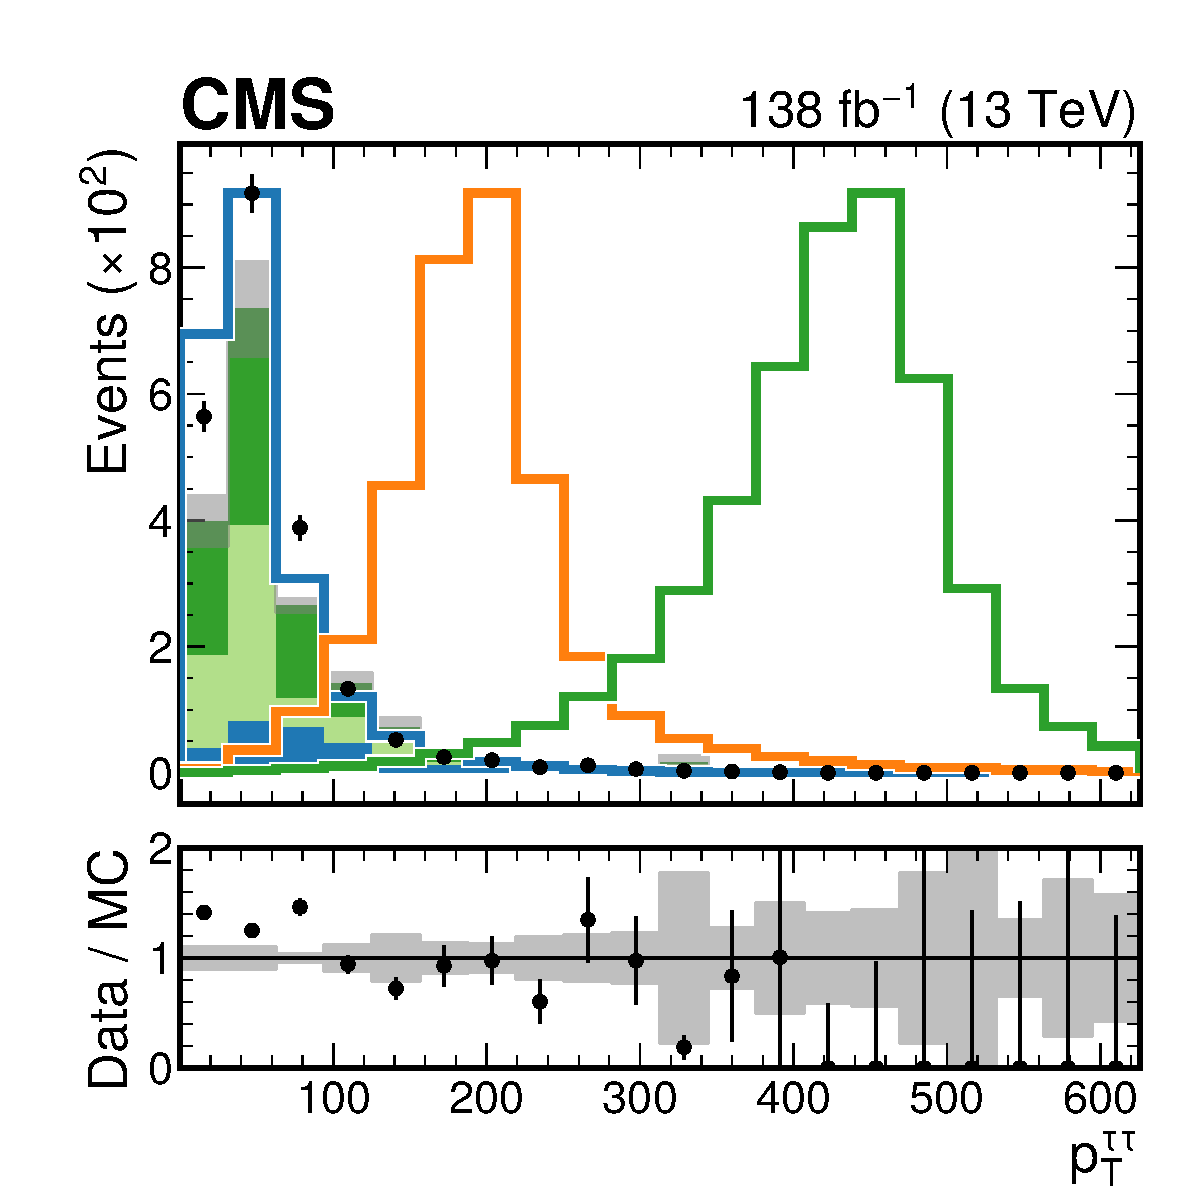
\includegraphics[width=.49\linewidth]{Figures/Dihiggs/categorisation/input_features/Graviton/Scale_equal/ditau_pt_GluGluToBulkGravitonToHHTo2G2Tau_M-1000_linear.pdf} \\
    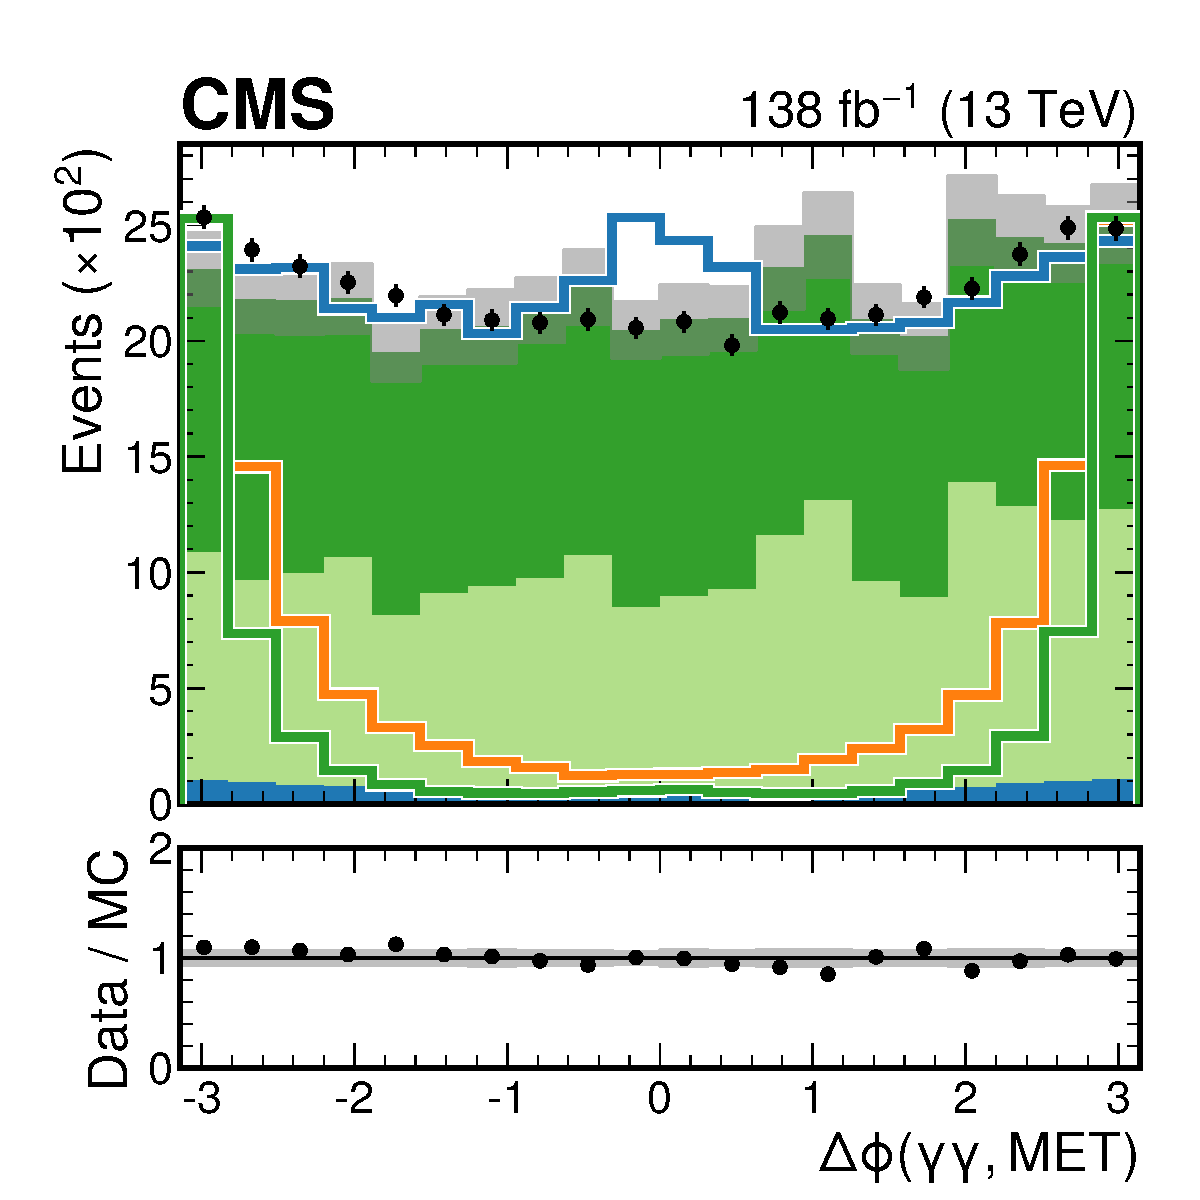
\includegraphics[width=.49\linewidth]{Figures/Dihiggs/categorisation/input_features/Graviton/Scale_equal/diphoton_met_dPhi_GluGluToBulkGravitonToHHTo2G2Tau_M-1000_linear.pdf}
    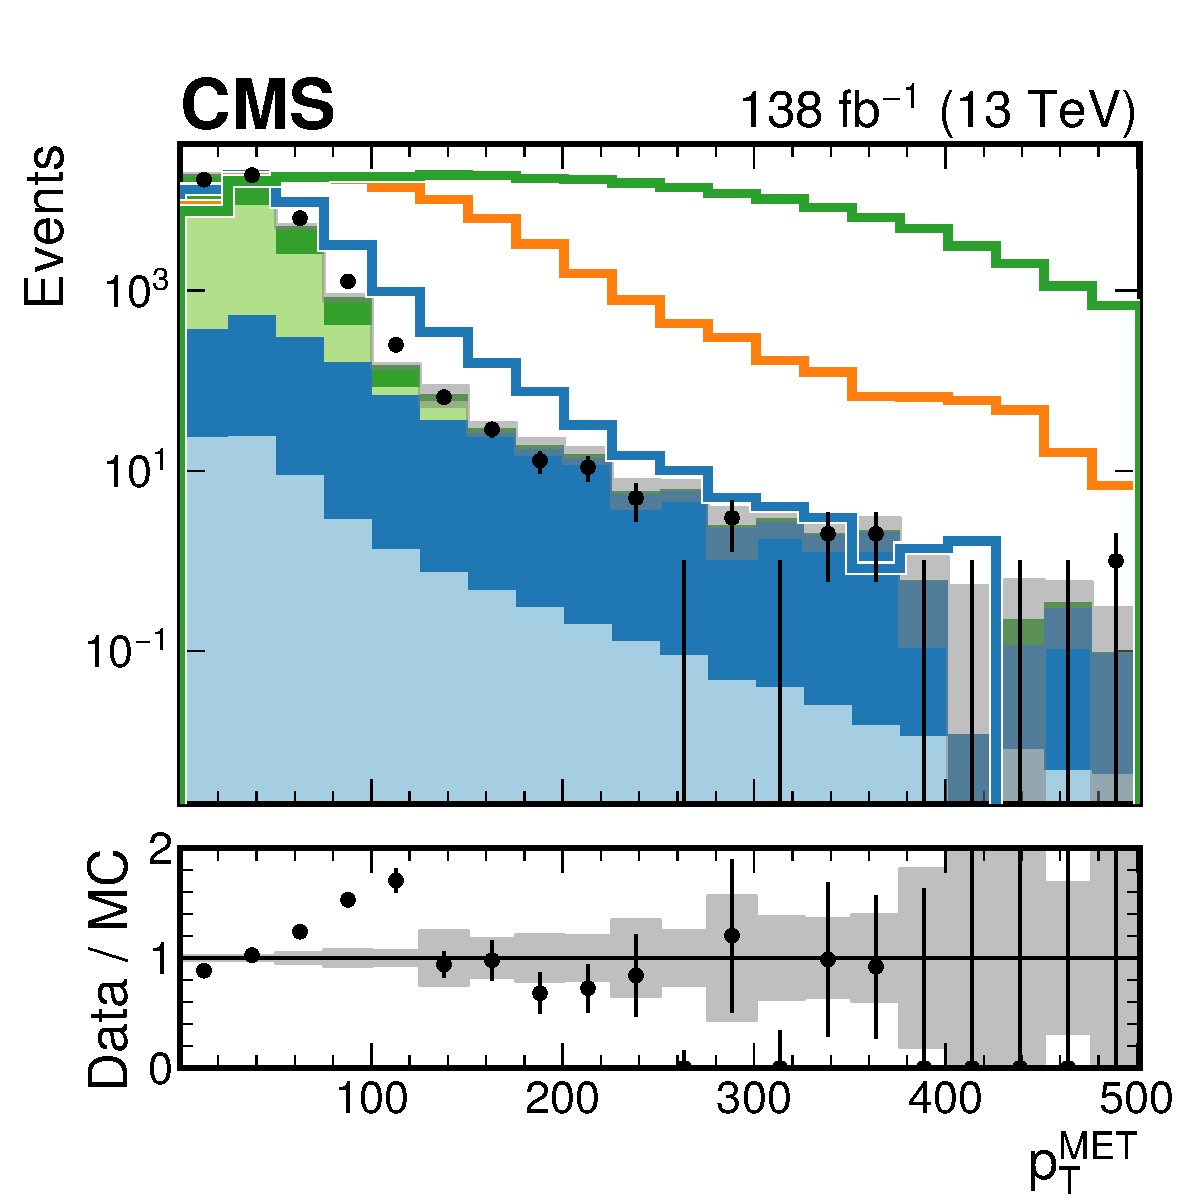
\includegraphics[width=.49\linewidth]{Figures/Dihiggs/categorisation/input_features/Graviton/Scale_equal/MET_pt_GluGluToBulkGravitonToHHTo2G2Tau_M-1000_log.pdf} \\
    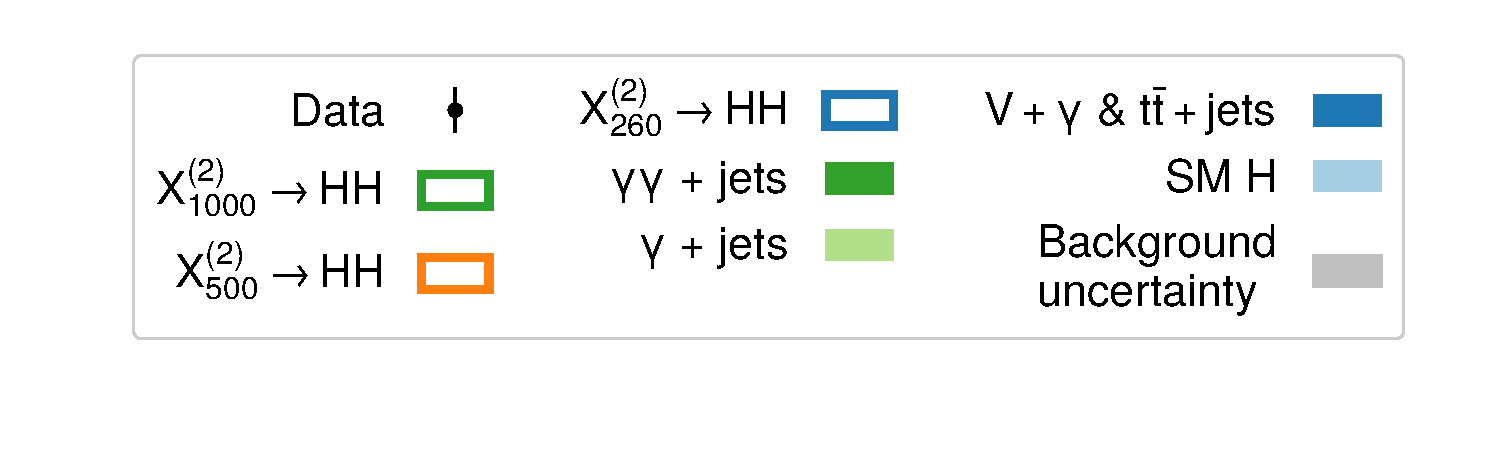
\includegraphics[width=.7\linewidth]{Figures/Dihiggs/categorisation/input_features/Graviton/Scale_equal/legend.pdf}
    \caption[Distributions of Training Features (5)]{Distributions of data, background MC, and \XTwoHH signals for $\mX=260$, 700 and 1000\GeV, in a subset of the variables used to train the pNN. Background MC is normalized to data and the signal's normalization is arbitrary. The statistical uncertainty in the background simulation is shown by the grey shaded bands.}\label{fig:training_features_5}
\end{figure}

\begin{figure}
    \centering
    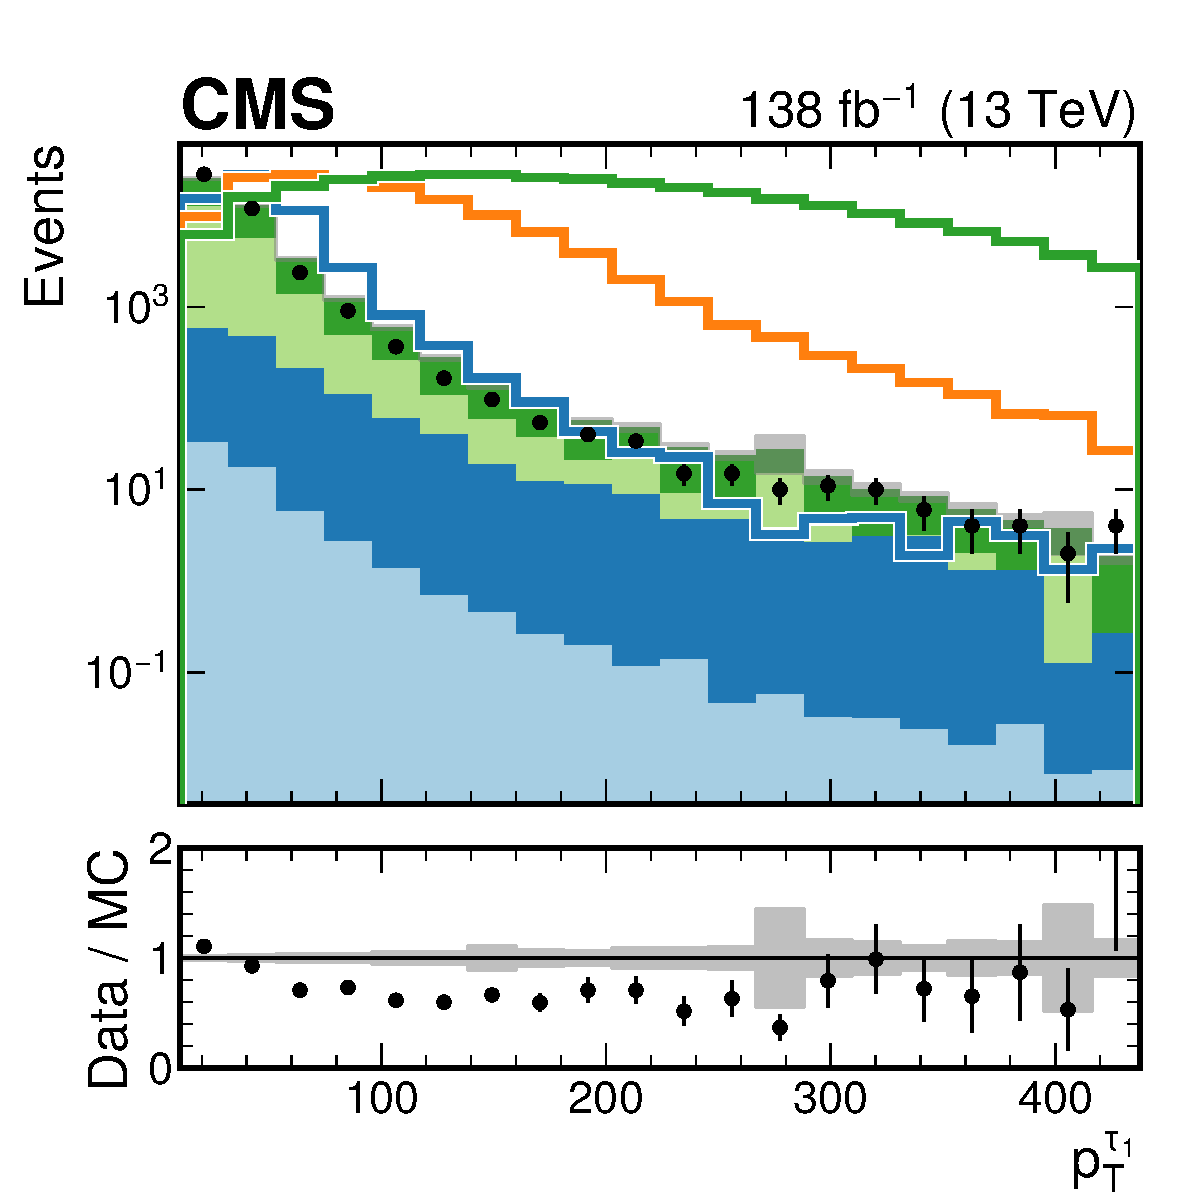
\includegraphics[width=.49\linewidth]{Figures/Dihiggs/categorisation/input_features/Graviton/Scale_equal/lead_lepton_pt_GluGluToBulkGravitonToHHTo2G2Tau_M-1000_log.pdf}
    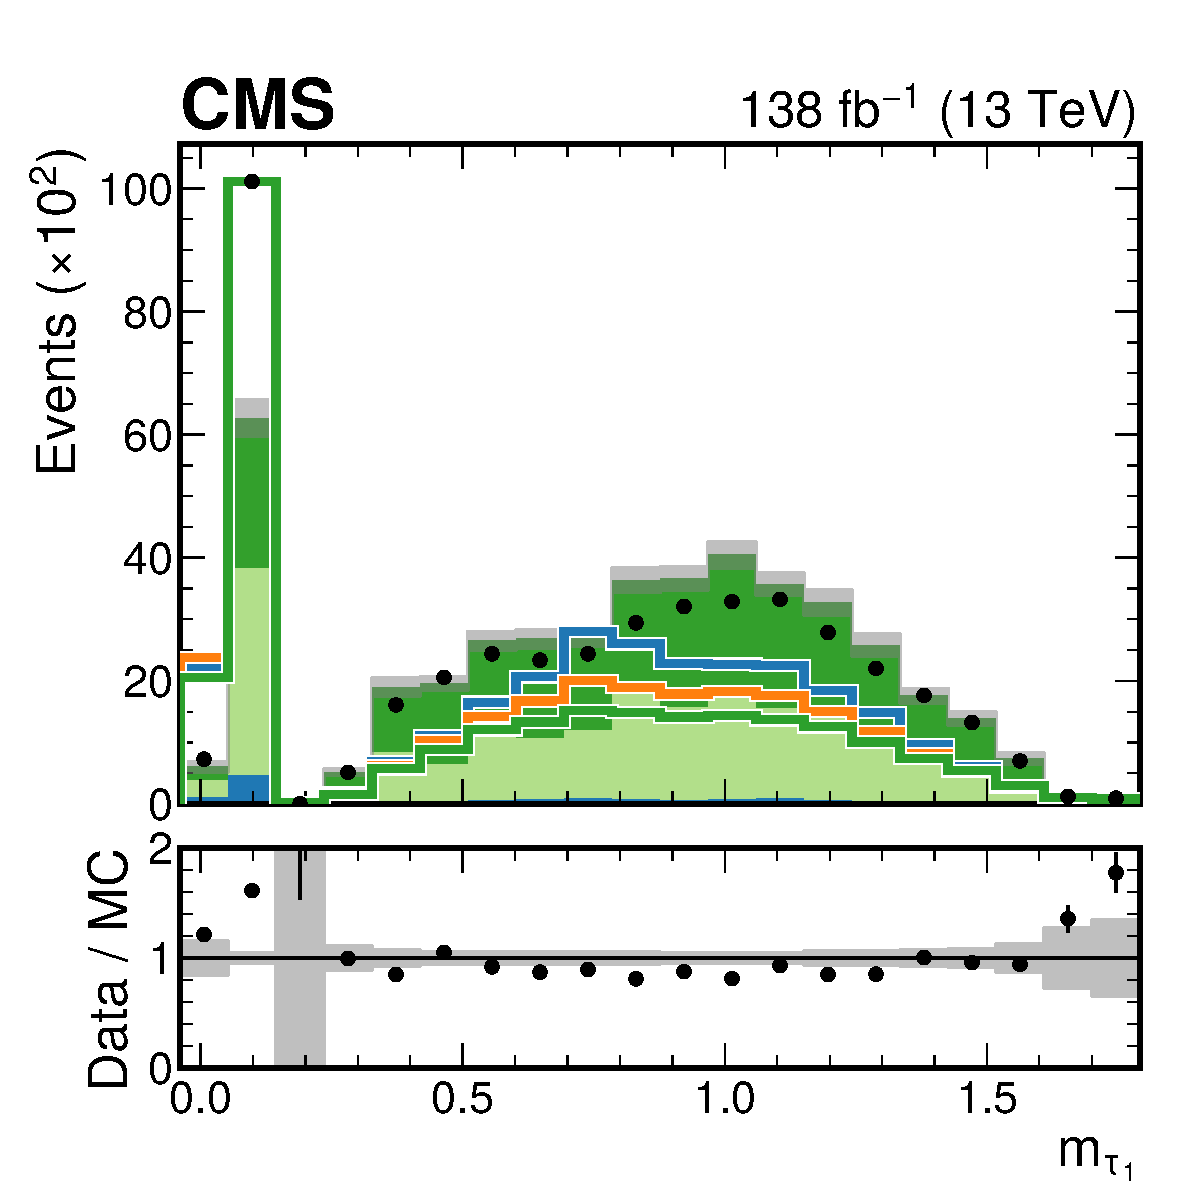
\includegraphics[width=.49\linewidth]{Figures/Dihiggs/categorisation/input_features/Graviton/Scale_equal/lead_lepton_mass_GluGluToBulkGravitonToHHTo2G2Tau_M-1000_linear.pdf} \\
    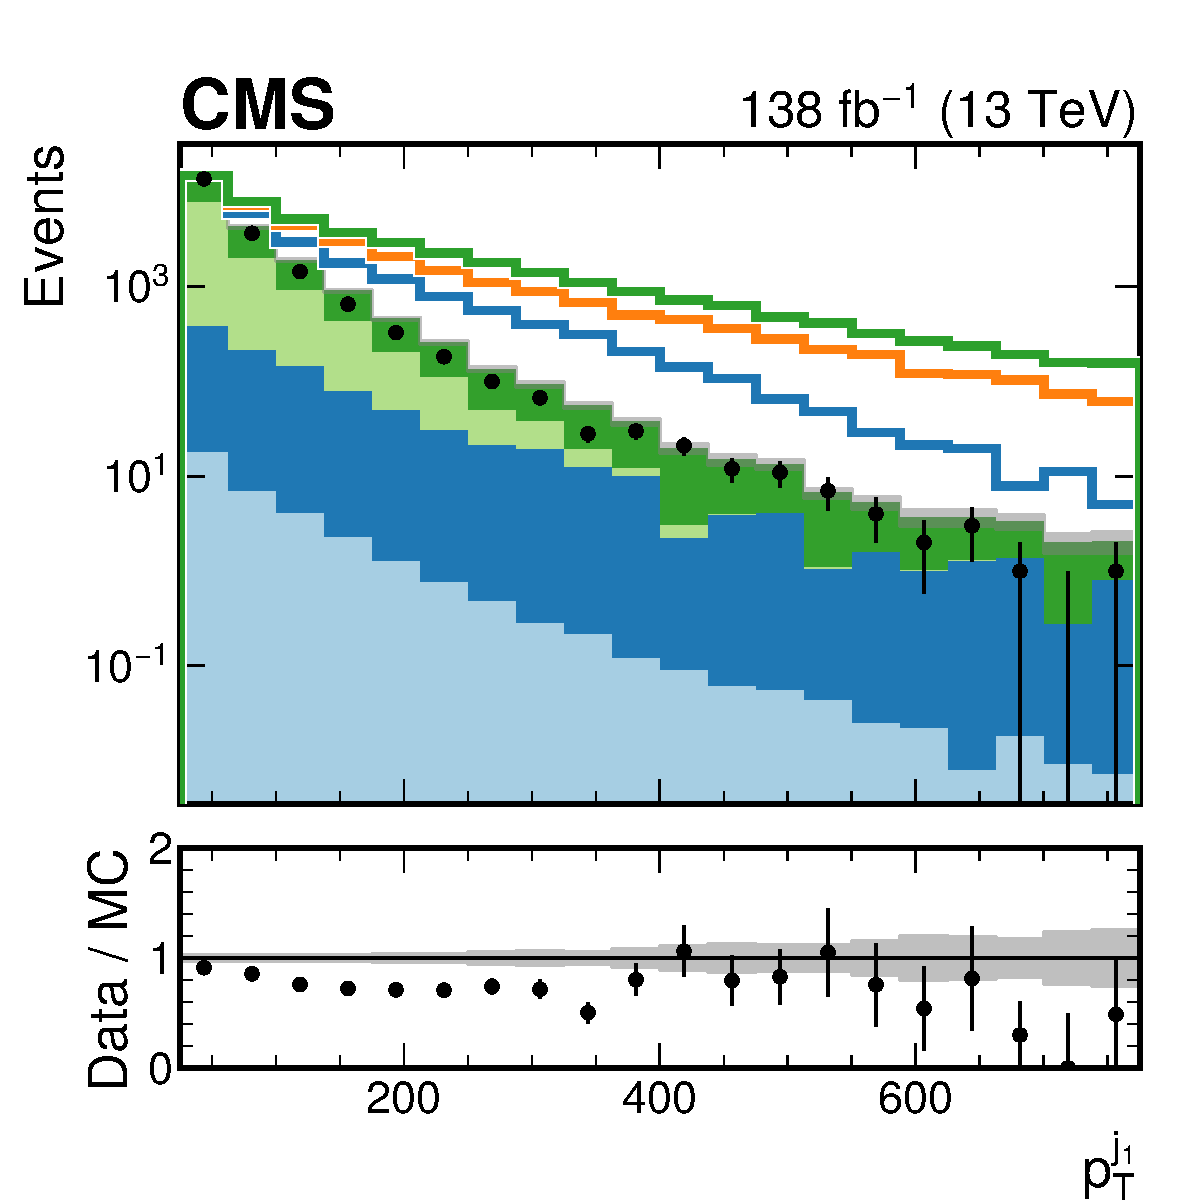
\includegraphics[width=.49\linewidth]{Figures/Dihiggs/categorisation/input_features/Graviton/Scale_equal/jet_1_pt_GluGluToBulkGravitonToHHTo2G2Tau_M-1000_log.pdf}
    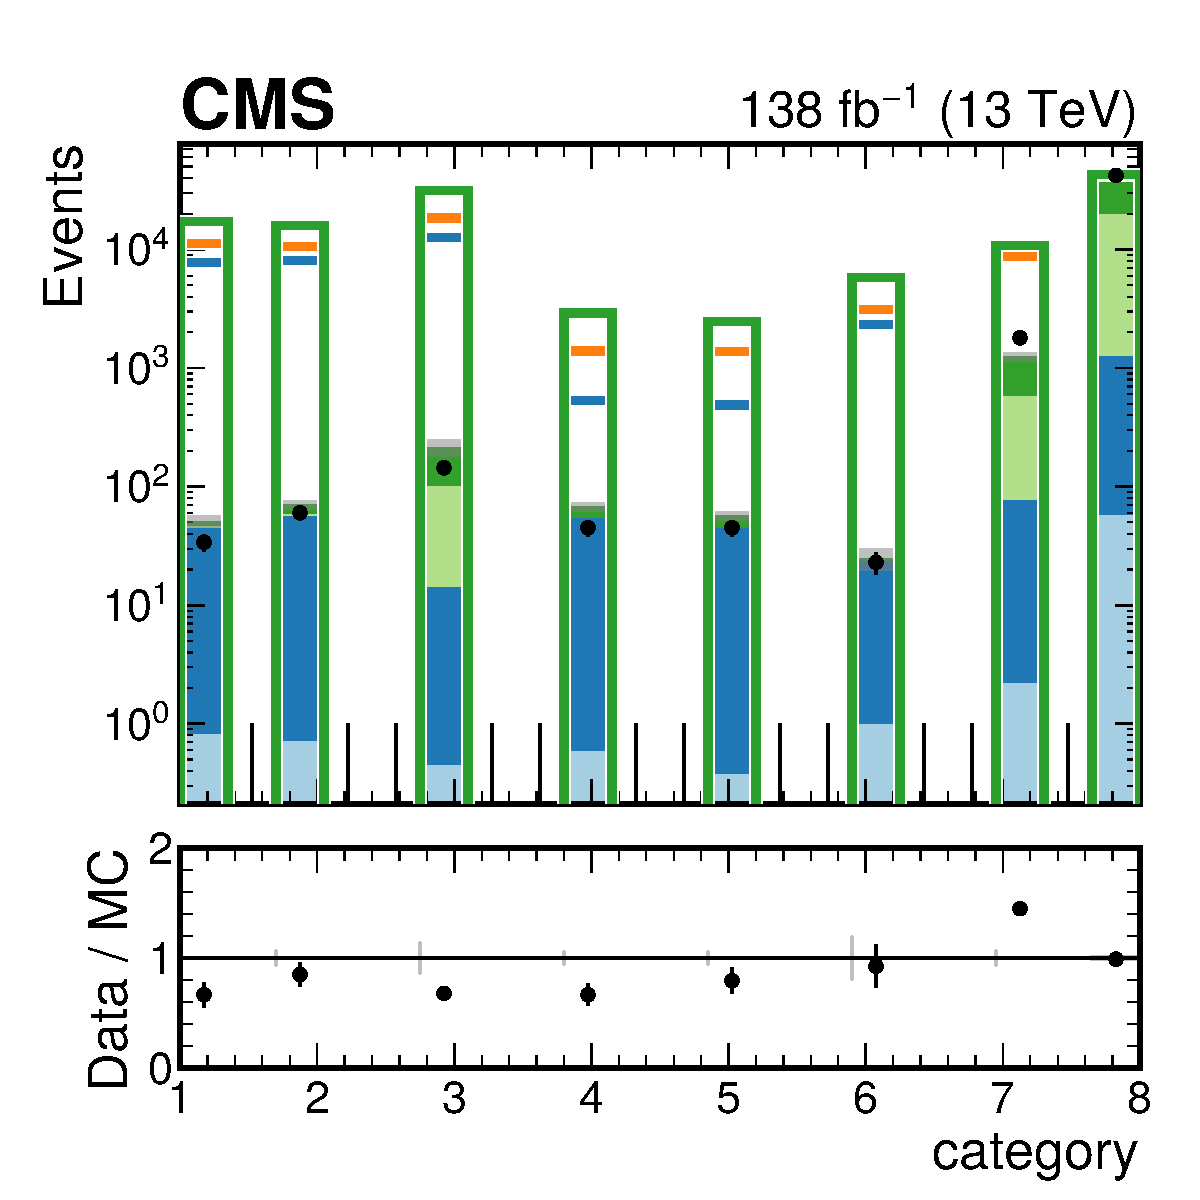
\includegraphics[width=.49\linewidth]{Figures/Dihiggs/categorisation/input_features/Graviton/Scale_equal/category_GluGluToBulkGravitonToHHTo2G2Tau_M-1000_log.pdf} \\
    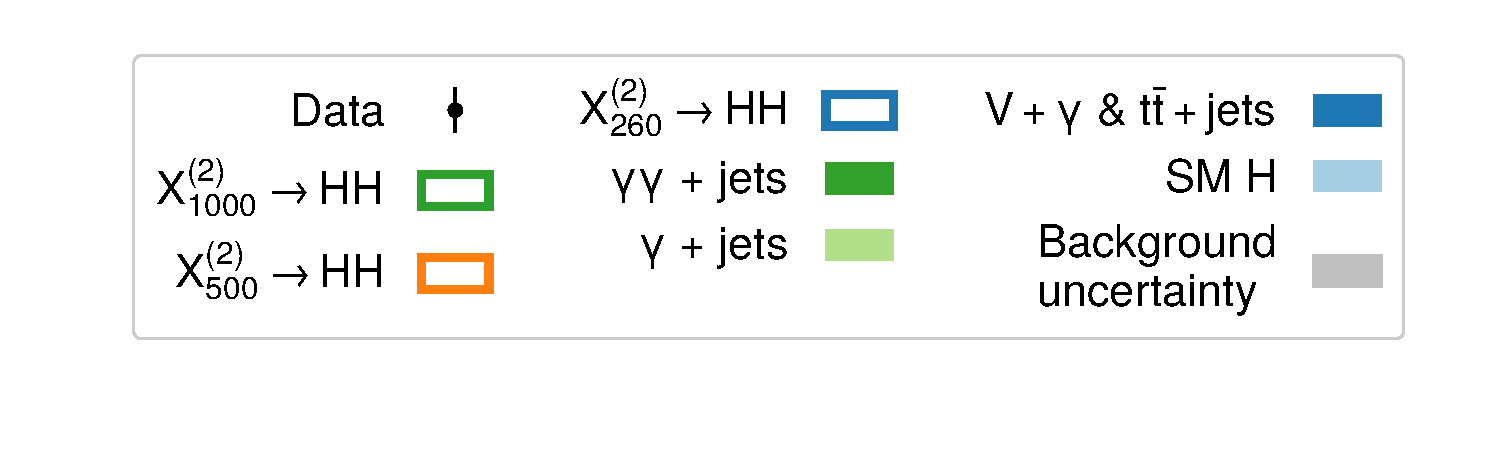
\includegraphics[width=.7\linewidth]{Figures/Dihiggs/categorisation/input_features/Graviton/Scale_equal/legend.pdf}
    \caption[Distributions of Training Features (6)]{Distributions of data, background MC, and \XTwoHH signals for $\mX=260$, 700 and 1000\GeV, in a subset of the variables used to train the pNN. Background MC is normalized to data and the signal's normalization is arbitrary. The statistical uncertainty in the background simulation is shown by the grey shaded bands. The bottom-right plot shows the channel of an event, where the numbering scheme is given in \cref{tab:channel}.}\label{fig:training_features_6}
\end{figure}

\begin{figure}
    \centering
    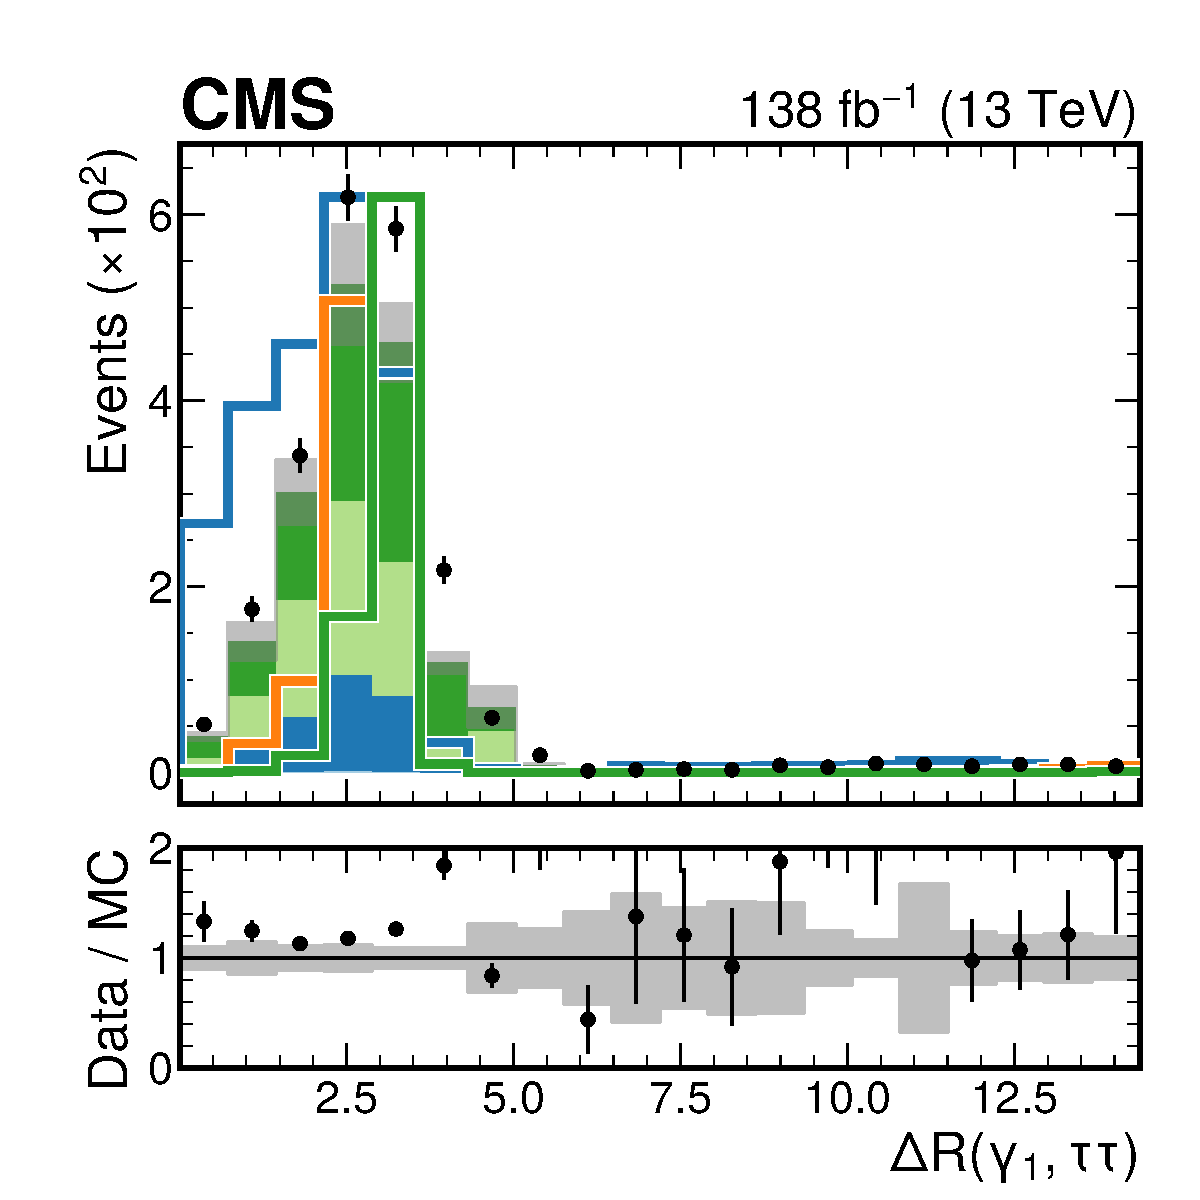
\includegraphics[width=.49\linewidth]{Figures/Dihiggs/categorisation/input_features/Graviton/Scale_equal/LeadPhoton_ditau_dR_GluGluToBulkGravitonToHHTo2G2Tau_M-1000_linear.pdf}
    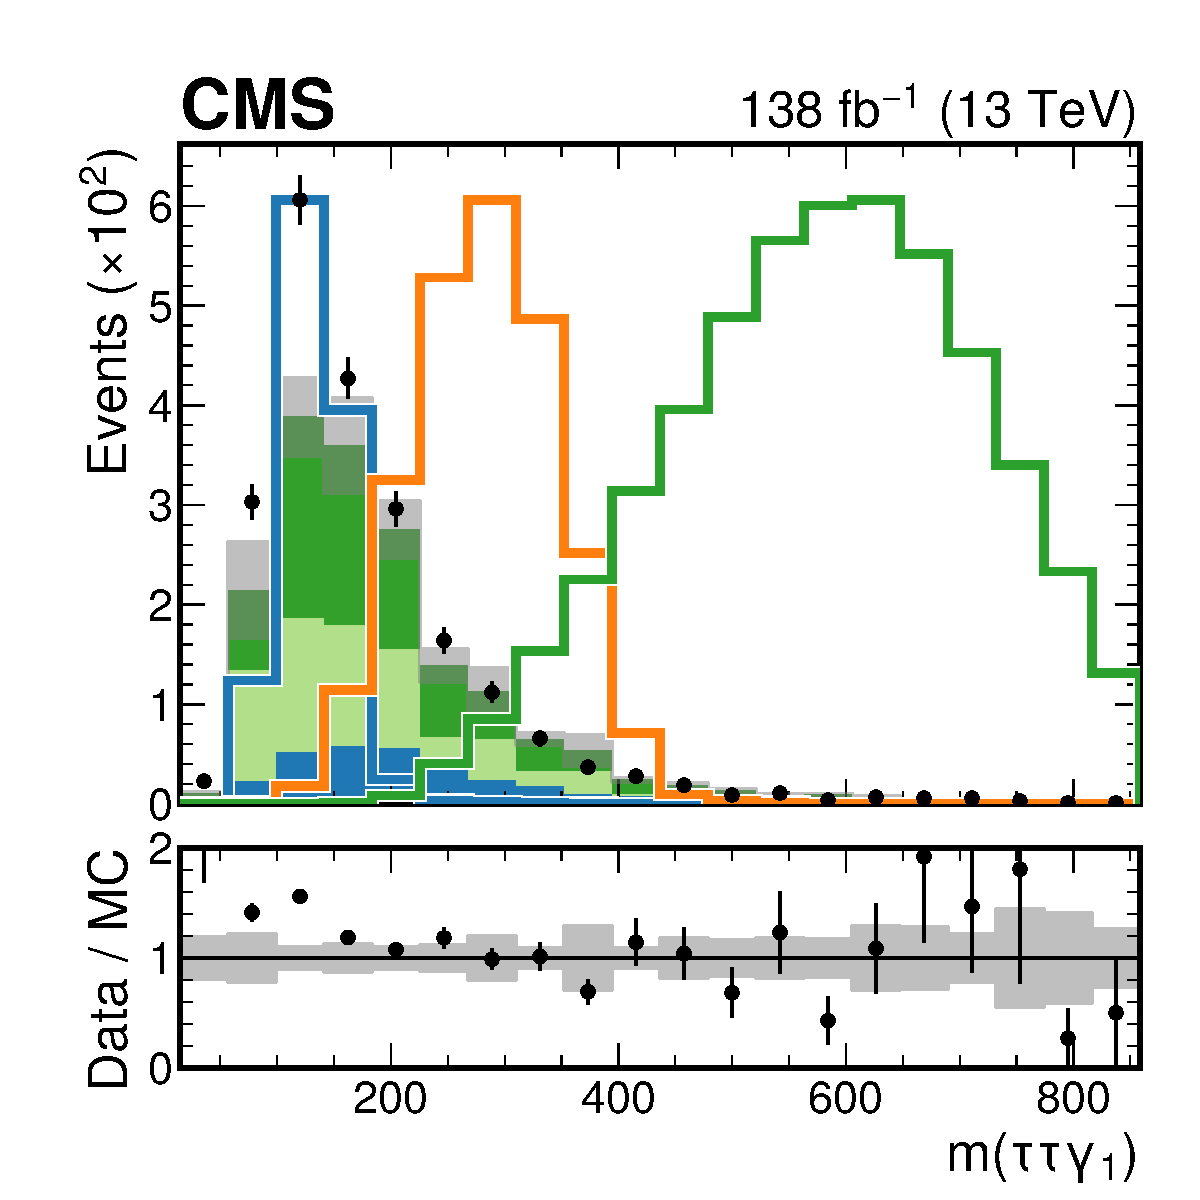
\includegraphics[width=.49\linewidth]{Figures/Dihiggs/categorisation/input_features/Graviton/Scale_equal/dilep_leadpho_mass_GluGluToBulkGravitonToHHTo2G2Tau_M-1000_linear.pdf} \\
    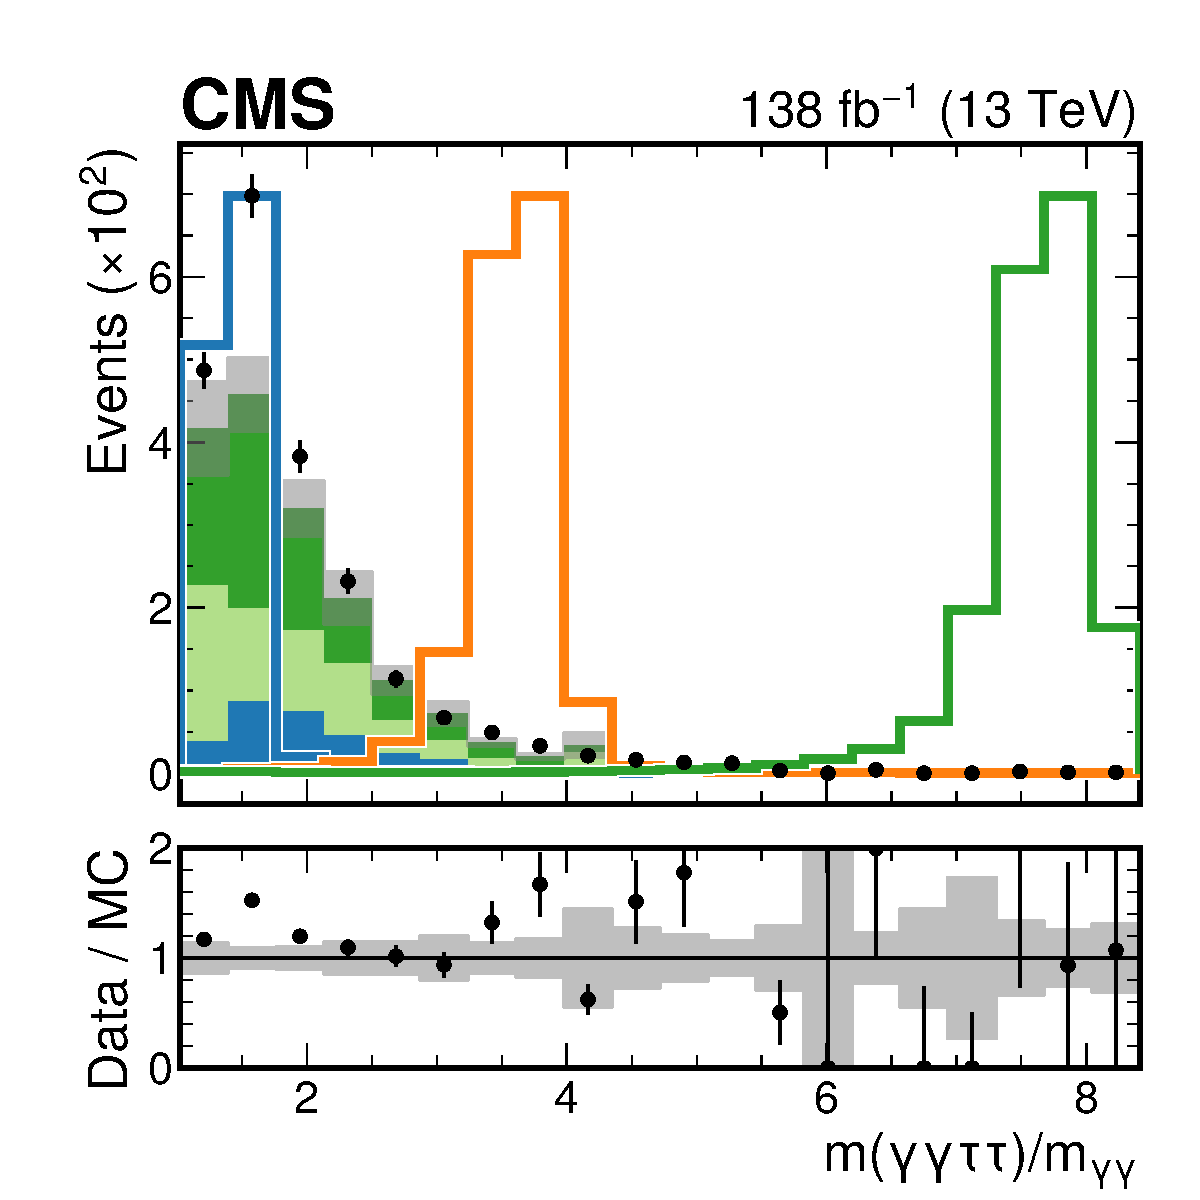
\includegraphics[width=.49\linewidth]{Figures/Dihiggs/categorisation/input_features/Graviton/Scale_equal/reco_MX_mgg_GluGluToBulkGravitonToHHTo2G2Tau_M-1000_linear.pdf} \\
    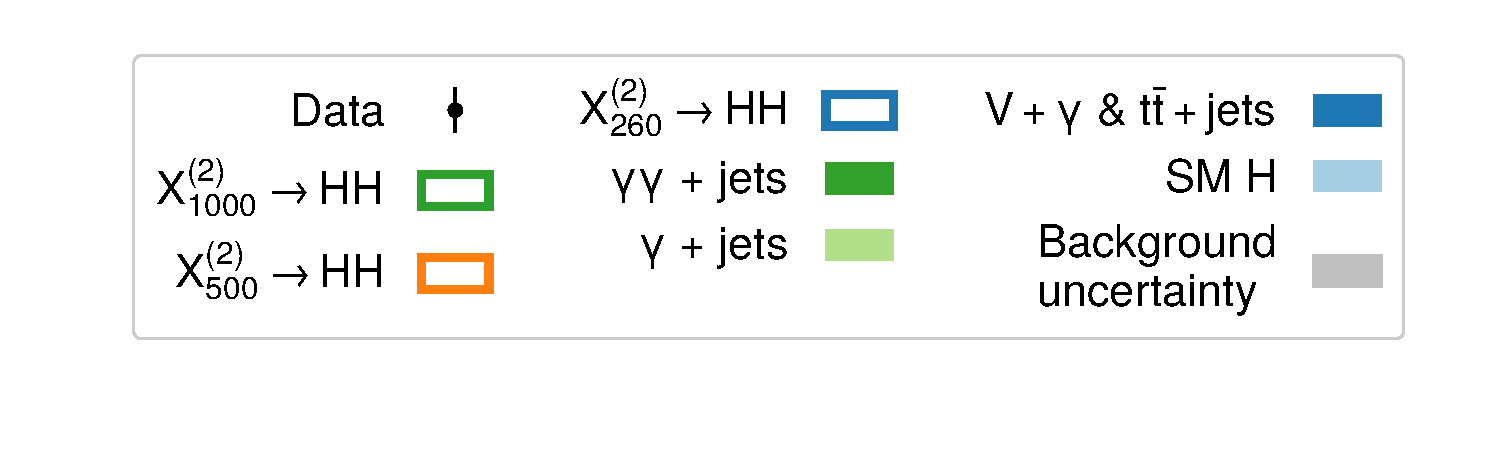
\includegraphics[width=.7\linewidth]{Figures/Dihiggs/categorisation/input_features/Graviton/Scale_equal/legend.pdf}
    \caption[Distributions of Training Features (7)]{Distributions of data, background MC, and \XTwoHH signals for $\mX=260$, 700 and 1000\GeV, in a subset of the variables used to train the pNN. Background MC is normalized to data and the signal's normalization is arbitrary. The statistical uncertainty in the background simulation is shown by the grey shaded bands.}\label{fig:training_features_7}
\end{figure}

\subsection{Parametric Neural Networks}\label{sec:pNN}

In analyses like this one where there are different target signals and many different resonance masses to search for, there are several approaches available to help discriminate signal from background. Examples include:
\begin{enumerate}
    \item Training a classifier for every target signal and every mass point. In this approach, every combination of process and mass point is treated as a separate analysis whose job is to only target this specific signal. This approach lends itself to good sensitivity since each analysis can be optimized to its signal without compromise introduced by the consideration of other processes and mass points. However, in this analysis, this would lead to the training of 208 classifiers in total and doing this, including hyperparameter optimization, could be a lengthy task. 
    \item Training a single classifier for all the processes and all the mass points. In this approach, all the signal MC is included in the training at once. Whilst this simplifies the classifier training, it is also non-optimal since it applies the same logic to discriminate against all the different signals. A more sensible approach would be to train a classifier per process with all mass points included, but this would still not be as optimal as approach 1.    
    \item Grouping together signals which are kinematically similar. Here, multiple classifiers would be trained per process, where each classifier is designed to target a particular kinematic regime. This is the approach taken by a resonant $\mathrm{HH}\rightarrow bb\gamma\gamma$ analysis performed by the CMS collaboration where signals are grouped based upon a `boost factor' defined as $\mX/(\mH+\mY)$~\cite{CMS:2023boe}. This represents a compromise between approach 1, which is more sensitive but also more complex, and approach 2, which is more simple but less sensitive.
\end{enumerate}
An alternative to the approaches described above are Parameterized Neural Networks (pNNs)~\cite{Baldi:2016fzo}. Per process, a single pNN could be trained that would, in principle, be as optimal as the first approach described above. This is possible because the pNN can change how it uses the discriminating (training) features depending on the value of a mass parameter(s). In more colloquial terms, it changes how to discriminate signal from background depending on the mass point it is asked to discriminate for.

To understand how a pNN works, first consider one of the \XHH processes, and a NN trained on a single mass point. This network is a function, $f(\vec{x})$, which can be roughly thought of as the probability that an event, described by training features, $\vec{x}$, is signal. If following approach 1, one would have a set of such functions $\{f^1, f^2,\cdots\}$ where $f^i$ is a NN trained with signal samples corresponding to $\mX^i$. One could put these functions together to create: 
\begin{equation}
f(\vec{x}; \mX) = 
\left\{ 
  \begin{array}{ c l }
    f^1(\vec{x}) & \quad \textrm{if } \mX=m^1 \\
    f^2(\vec{x}) & \quad \textrm{if } \mX=m^2 \\
    \vdots & \quad \quad \quad \vdots 
  \end{array}
\right\}.\label{eqn:combined_fx}
\end{equation}
When using this function, picking a value of \mX is equivalent to picking a particular NN to use. When training a pNN, the target function \textit{is} $f(\vec{x}; \mX)$, i.e.\ a single function, which given a value of \mX, will provide a discriminator specific to that value of \mX. In practice, this is achieved by:
\begin{enumerate}
    \item Including \mX as an additional training feature (this is a different feature to the reconstructed \mX features described in \cref{sec:training_features}).
    \item Training the NN on all of the signal MC simultaneously where the events are assigned a value of \mX which corresponds to the dataset they originated from, i.e.\ events from the $\mX=300$ GeV dataset will be given a value of 300 for the training feature \mX. 
    \item Constructing training batches such that there are an equal number of signal events and background events in each batch. Then, randomly pairing each signal event with a background event in the batch and giving the background event the same value of \mX as the signal event. This ensures that on a per-batch basis, that there is no power to discriminate between signal and background using the \mX training feature.
    \item Renormalizing the signal datasets ($\mX=300,400,\ldots,1000$\GeV) such that the sum of weights in each is the same.
    \item Renormalizing the signal (all masses collectively) and background datasets such that the sum of weights is the same between the two.
\end{enumerate}
The last two steps are not necessary to make a network parametric in \mX, but they ensure that the network is not biased towards any particular mass point and lead to better overall performance.

It is possible to gain an intuition about what the pNN is doing implicitly. Consider a network trained on a single mass point. At each layer in the network, more complicated features can be made from the outputs of the previous layer. At the end of the network, these features are combined to make a single discriminator, $f(\vec{x})$. If \mX is included as a training feature, then the features can be made to change depending on \mX. For example, the mean value of a feature in signal may scale with \mX, e.g. $m(\ggtt)$ or $\pt^{\gamma\gamma}$. By including \mX in the network, it is possible that features such as $x_1= \mX - m(\ggtt)$ or $x_2 = \mX - a*\pt^{\gamma\gamma}$ ($a \in \mathbb{R}$) could be created. Then, the network could give high scores to events where $x_1$ and $x_2$ are close to zero.

Another advantage to pNNs is their ability to interpolate between mass points. Unlike \cref{eqn:combined_fx}, the function provided by a pNN is defined for all values for \mX. It is therefore possible that a pNN can be used to discriminate for mass points that were not seen during training. Consider training on $\mX=300$ and $400$\GeV. A pNN will learn how to discriminate for those two masses, and it could ``guess'' that to discriminate at $\mX=350$\GeV it must apply logic that is somewhere in between that used for 300 and 400\GeV. This concept is illustrated in \cref{fig:pNN_interpolation_intution}.

\begin{figure}
    \centering
    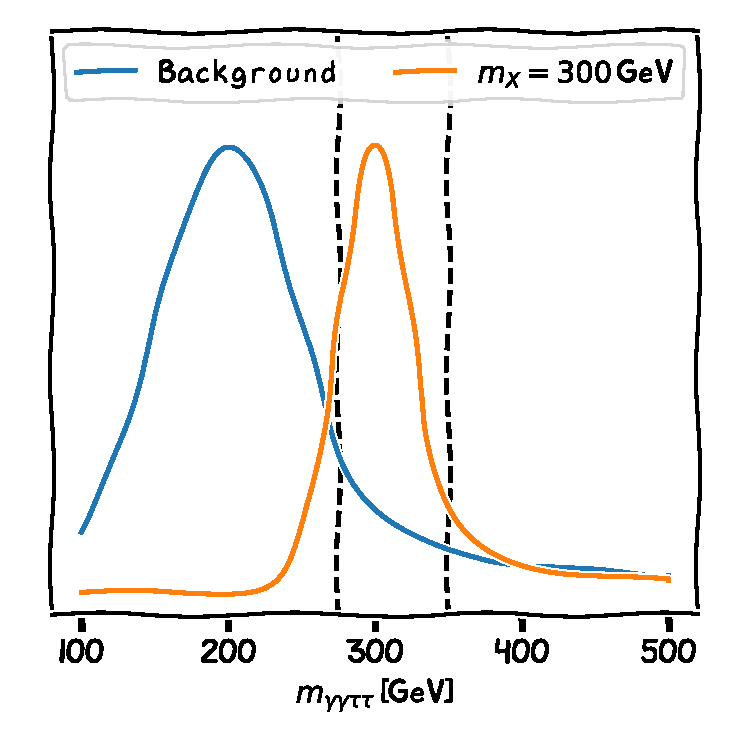
\includegraphics[width=0.32\textwidth]{Figures/Dihiggs/categorisation/pNN_intution_mX300.pdf}
    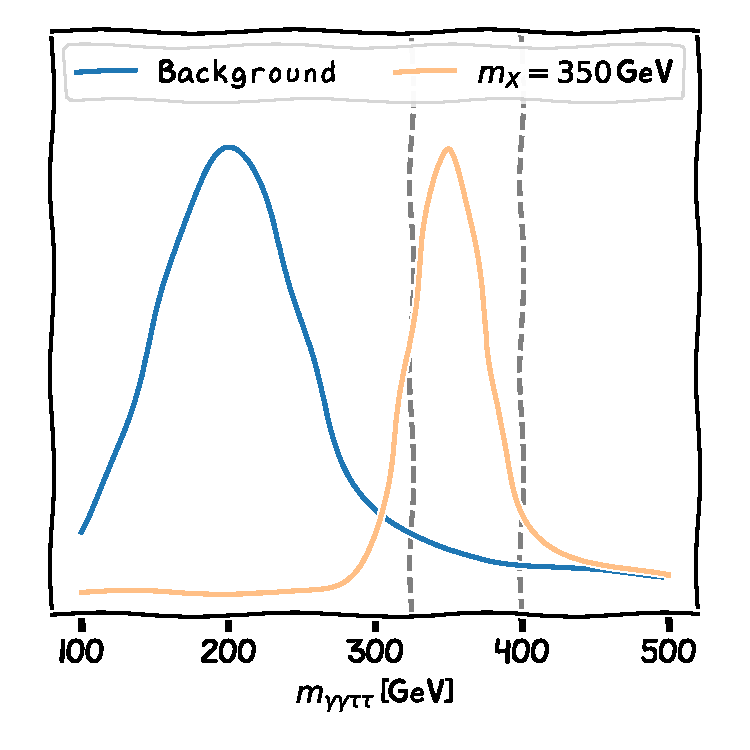
\includegraphics[width=0.32\textwidth]{Figures/Dihiggs/categorisation/pNN_intution_mX350.pdf}
    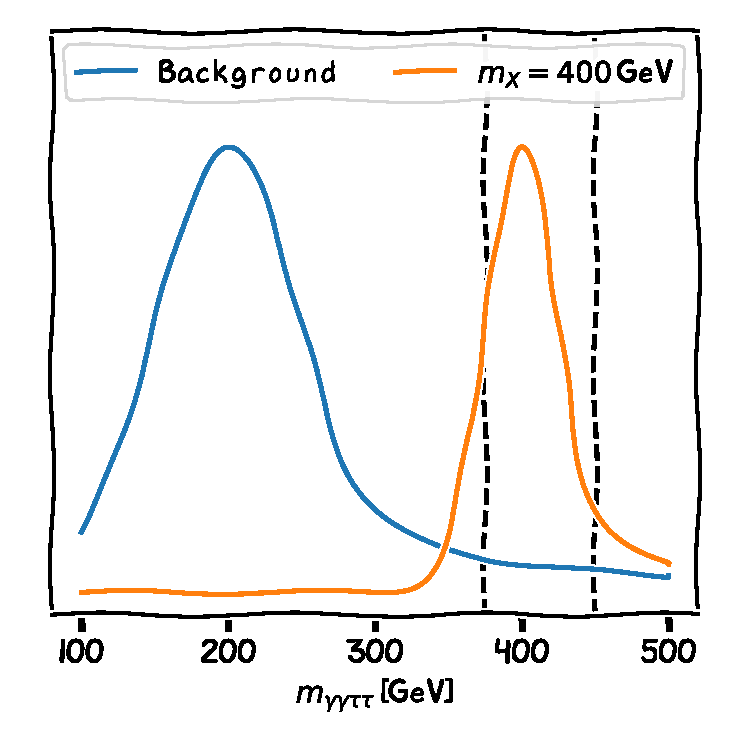
\includegraphics[width=0.32\textwidth]{Figures/Dihiggs/categorisation/pNN_intution_mX400.pdf}
    \caption[Illustration of pNN Interpolation Ability]{Toy examples of distributions of $m(\ggtt)$ in background and in signal for the $\mX=300$, 350 and 400\GeV \XHH signals. In each case, a selection represented by the dashed black lines on $m(\ggtt)$ is proposed to separate signal from background. This selection is used to illustrate the selection that a pNN may effectively apply to this variable. By training the pNN on the $\mX=300$ and 400\GeV signals, it may learn to apply a selection for the 350\GeV mass point that is somewhere between the selection used for 300 and 400\GeV.}\label{fig:pNN_interpolation_intution}
\end{figure}

\newpage\noindent
To justify their use in this analysis, a pNN must fulfil two criteria:
\begin{enumerate}
    \item Good performance at every mass point: when evaluating on individual mass points, the pNN performs similarly to using a set of NNs where each NN is trained only on a single mass point (as in approach 1),
    \item Good performance at interpolated mass points: the pNN is able to discriminate well at mass points which it has not been trained on and that are in the ranges of masses used during training.
\end{enumerate}
In \cref{sec:categorisation_performance}, tests are devised to investigate this and the degree to which the pNNs meet these criteria is presented.

For the NMSSM models, the pNNs must be parametric in \mX and \mY. This is done by introducing both \mX and \mY as training features instead of just \mX, and following the same techniques. 


\subsection{Training and Performance}\label{sec:categorisation_performance}

The pNN is implemented in \PyTorch~\cite{PyTorch} and is a multilayer perceptron network of 3 layers of 50 nodes activated by exponential linear unit (ELU) functions with a dropout probability of 0.05. A schematic is given in \cref{fig:pNN_architecture}. This architecture, was chosen after a grid search of the hyperparameters shown in \cref{tab:hyperparameters}. This optimization procedure was performed for the \XTwoHH search and the set of hyperparameters chosen were those that lead to high AUC scores for the $\mX=260$, 500 and 1000\GeV signals. With this set of hyperparameters as a baseline, further grid searches were performed on the other searches but no significant improvement in AUC scores was found by moving away from the baseline hyperparameters so the same hyperparameters were used for all searches.

\begin{figure}
    \centering
    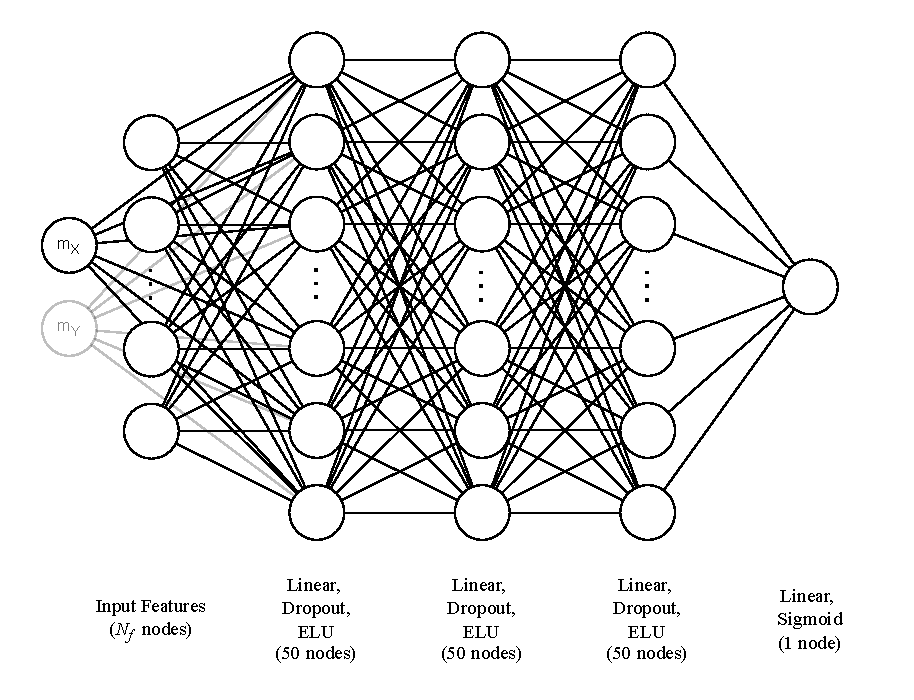
\includegraphics[width=\textwidth]{Figures/Dihiggs/nn_architecture.pdf}
    \caption[Architecture for the pNN]{Architecture for the pNN. The parametric features, \mX and \mY, are connected in the same way that the input features are, but are not included in the count of the input features, $N_f$. In the \XHH pNNs, the \mY node and connections do not exist, which is why they are drawn with a grey colour in the diagram. For the high-mass \XYggHtt search, $N_f=25$, and for all other searches, $N_f=27$.}\label{fig:pNN_architecture}
\end{figure}

\begin{table}
    \centering
    \begin{tabular}{cc}
    \toprule
        Number of layers & 2, 3, 4 \\ \midrule
        Number of nodes & 25, 40, 50, 60, 75 \\ \midrule
        Dropout probability & 0, 0.025, 0.05, 0.075, 0.1 \\ \bottomrule
    \end{tabular}
    \caption[Values of Hyperparameters Used in a Grid Search to Optimize the pNN Architecture]{Values of hyperparameters used in a grid search to optimize the pNN architecture.}\label{tab:hyperparameters}
\end{table}

In each search: \XZeroHH, \XTwoHH, \XYttHgg, low-mass \XYggHtt, and high-mass \XYggHtt, a pNN is trained using the features described in \cref{sec:training_features}. The number of events for the background processes, and for the signal processes in each search are summarized in \cref{tab:ggtt_training_dataset_num_events}. From these, 50\% of the events are reserved for testing and later for signal modelling, 40\% forms a training dataset used for loss minimization, and 10\% is used as a validation dataset used to track the pNN performance during training. 

During training, two of the background samples, \gjet and \ttbar, are not used, because despite having relatively high numbers of expected events in this analysis, the samples have small numbers of events which means that their inclusion reduces the effective statistical power of the dataset. This leads to overtraining and studies into the \XTwoHH analysis found a 5--13\% worsening to the expected upper limits with their inclusion. Similarly, negatively weighted events are excluded when training because their omission was found to lead to marginal improvements in the expected limits. 

\begin{table}
    \centering
    \begin{tabular}{ccc}
        \toprule
        Process & Number of events & Average per mass point \\ \midrule
        Background & 274K & \NA \\
        \XZeroHH & 625K & 37K \\
        \XTwoHH & 680K & 40K \\
        \XYttHgg & 7.5M & 82K \\
        Low-mass \XYggHtt & 2.9M & 73K \\
        High-mass \XYggHtt & 3.8M & 75K \\ \bottomrule
    \end{tabular}
    \caption[Sum of the Number of Background and Signal Events Across All Simulated Datasets]{Sum of the number of background and signal events across all simulated datasets.}\label{tab:ggtt_training_dataset_num_events}
\end{table}

The network is trained by minimizing the average binary cross entropy (BCE) loss function:
\begin{equation}
    -\frac{1}{N} \sum_i^N w_i \left[ y_i \log(f(\vec{x}_i; \mX^i, \mY^i)) + (1-y_i)\cdot\log(1-f(\vec{x}_i; \mX^i, \mY^i)) \right]
\end{equation}
where the sum is over $N$ events, $f(\vec{x};\mX, \mY)$ is the network output, $w_i$ is the event weight, and $y$ is a truth label that is equal to zero for background events and one for signal events. The minimization is performed using the \ADAM optimizer~\cite{Adam} with a batch size of 128 and an initial learning rate of 0.01 which is reduced by a factor of 0.9 at every epoch where the training loss does not decrease. These values of the training hyperparameters were found to lead to good performance and reasonably-fast convergence of the loss function. Changes around these values did not lead to substantially different performance which is why they were not included in the grid search of hyperparameters discussed previously. 

Batches are constructed by randomly sampling, without replacement, 64 events from the signal component of the training dataset and 64 events from the background component. When sampling events from the signal or background components, the weights of events are taken into account and therefore, the events are treated as unweighted in the BCE loss calculation for the batch. An epoch is defined as one pass through the background component of the dataset. 

The evolution of the loss on the training and validation datasets when training the \XTwoHH pNN is shown in \cref{fig:pNN_loss_graviton}. To gain insight into the pNN training, the training and validation datasets are split according to the signal processes where an equal number of background events are given to each split, and the losses over each split are studied. These losses for $\mX = 260$, 500 and 1000\GeV are also shown in \cref{fig:pNN_loss_graviton}. As expected, the overall contribution to the loss at the end of training is greatest from the 260\GeV dataset since this signal is more difficult to discriminate for than the 500 or 1000\GeV signals. Furthermore, greater improvements to the loss are seen in the 260\GeV dataset over the training duration which implies that the training was driven more by the 260\GeV signal than the 500 and 1000\GeV signals. Or in other words, there was more that had to be learned for the lower $\mX$ signals than the higher $\mX$ signals. The loss evolution of the pNNs for the other searches are shown in \cref{fig:pNN_loss_rest}.

The training duration is determined by the validation dataset. During training, the pNN parameters are saved to disk after each epoch, and the individual validation losses for every signal process are tracked. If no relative improvement of $>0.1\%$ is seen in any of the losses over a 15 epoch period, then the training is stopped. This ensures that the training is not stopped whilst there is a signal process for which the discrimination is still improving. Finally, the pNN parameters from the epoch with the lowest total validation loss are used. 

\begin{figure}
    \centering
    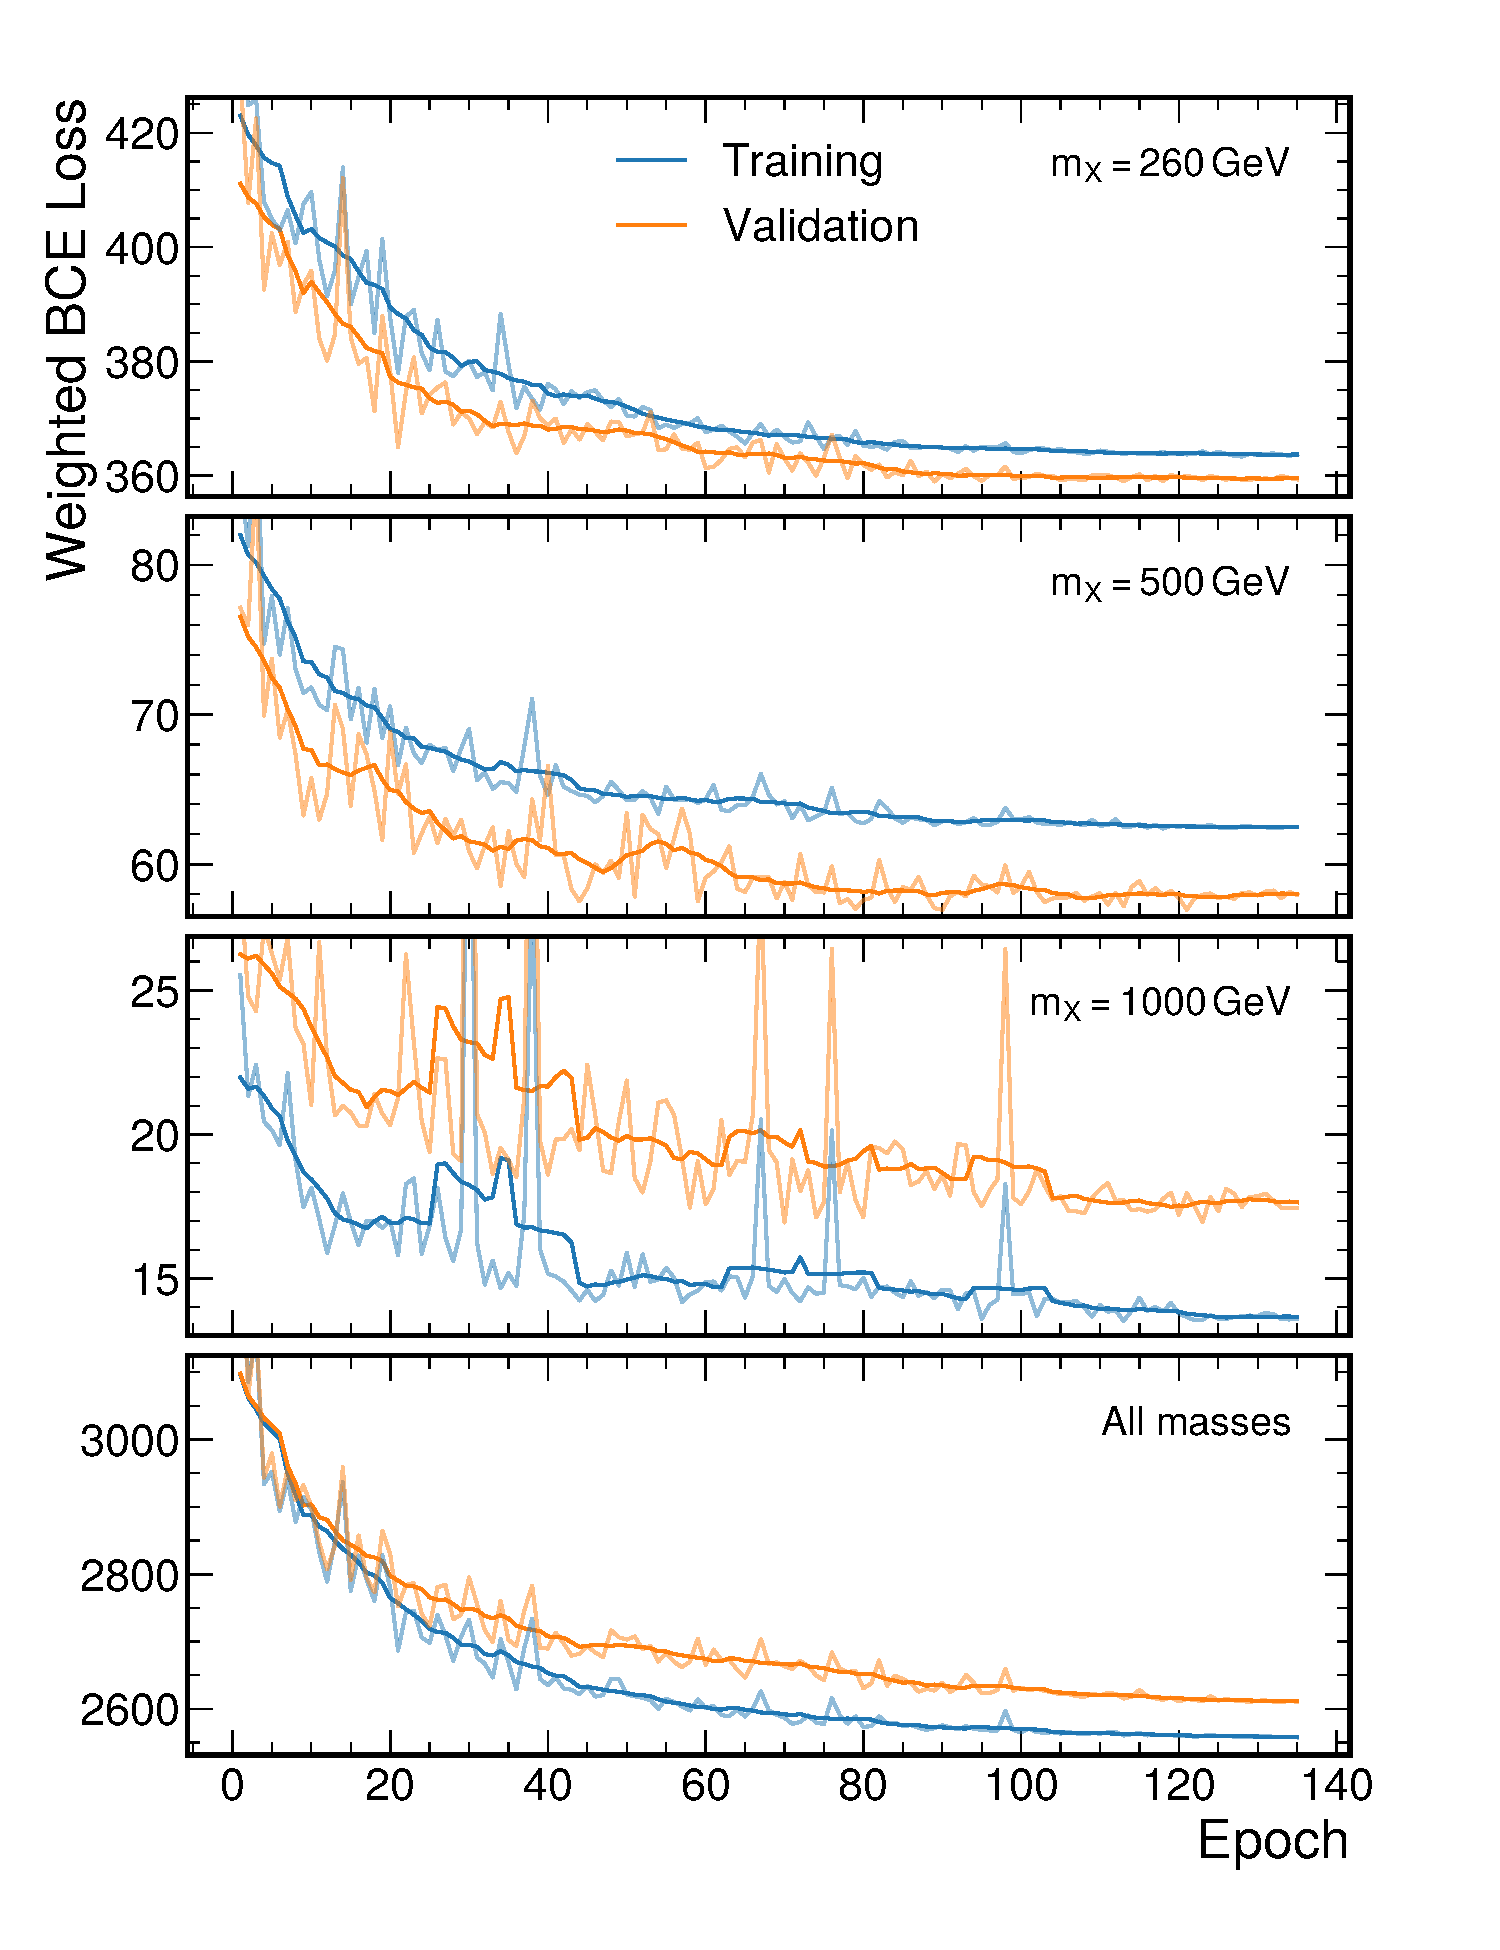
\includegraphics[width=0.8\textwidth]{Figures/Dihiggs/categorisation/graviton_loss_split.pdf}
    \caption[Evolution of BCE Loss for the \XTwoHH pNN Split by Mass Point]{Total (not averaged) BCE loss for the \XTwoHH pNN after every epoch of training for both the training and validation datasets. The datasets are split into components corresponding to the $\mX = 260$, 500, and 1000\GeV signals and the corresponding losses are shown in the top three plots, with the loss over the whole datasets shown in the bottom plot. The total normalization of the dataset, and therefore, the scale of the loss, is arbitrary, but the normalization of each signal component is equal. The first loss values shown at Epoch 1 correspond to the losses after 1 epoch of training. The opaque lines represent a rolling average in a centred window of 10 epochs of the true loss values, shown by the faint lines of the same colour.}\label{fig:pNN_loss_graviton}
\end{figure}

\begin{figure}
    \centering
    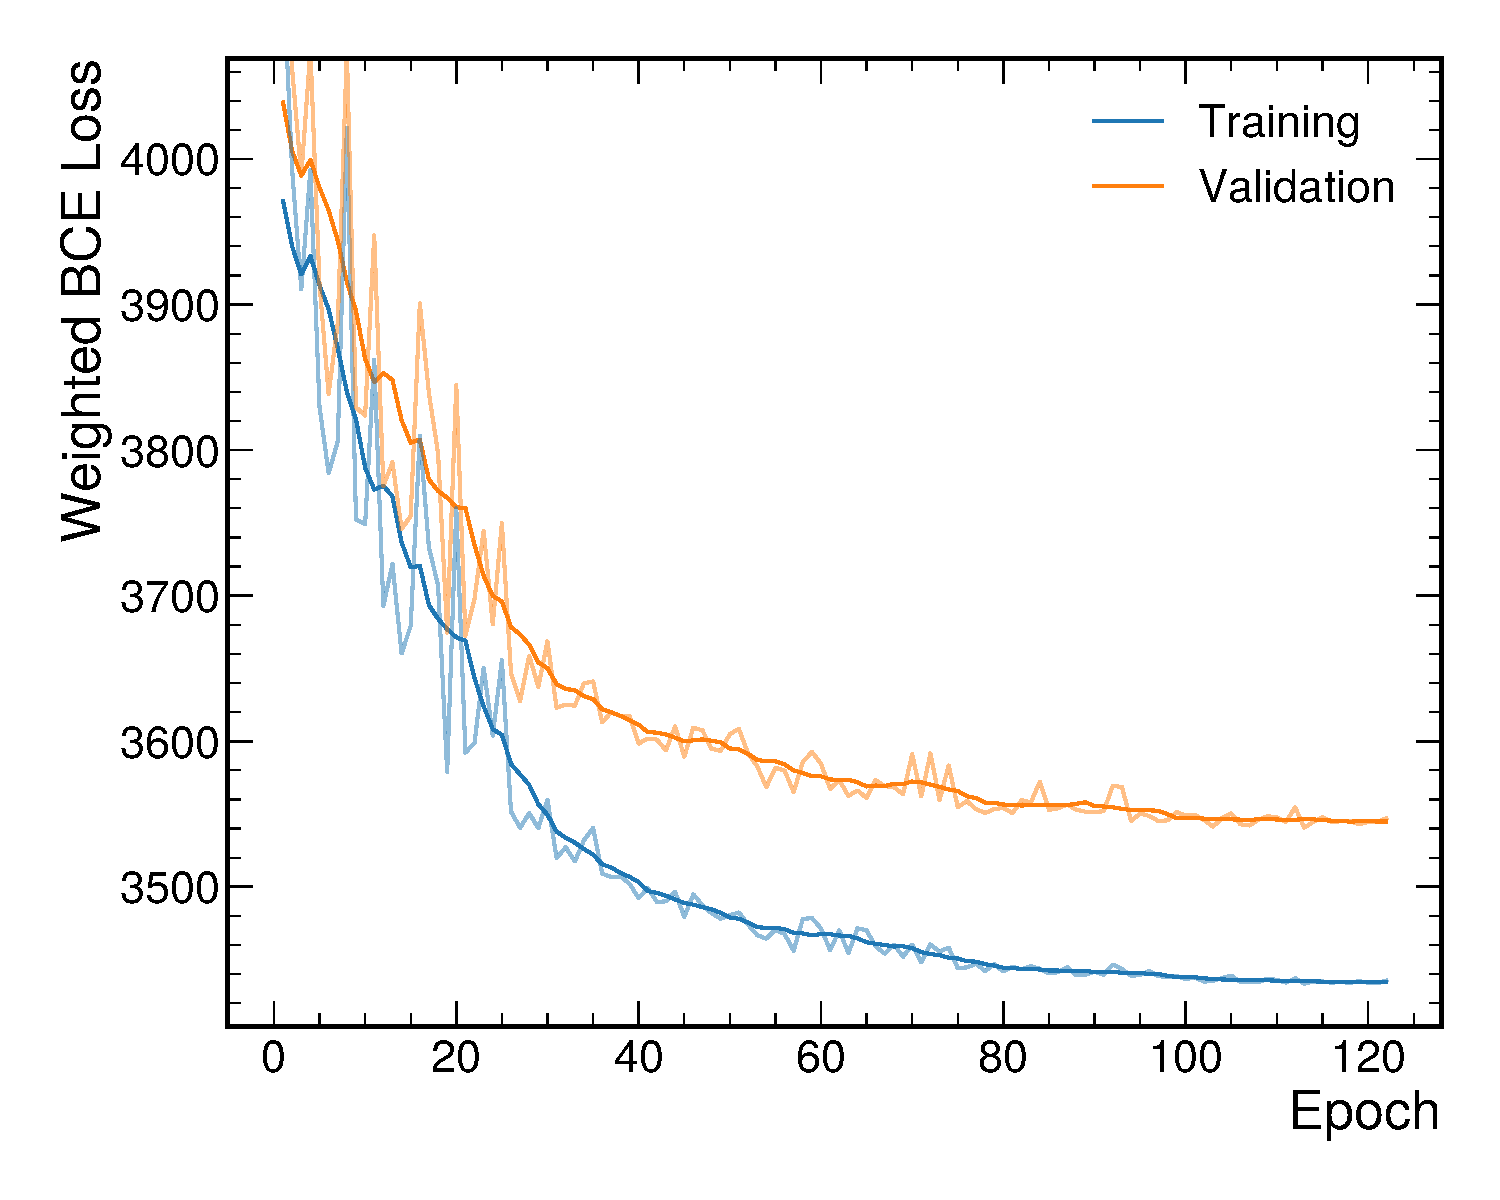
\includegraphics[width=0.49\textwidth]{Figures/Dihiggs/categorisation/radion_loss.pdf}
    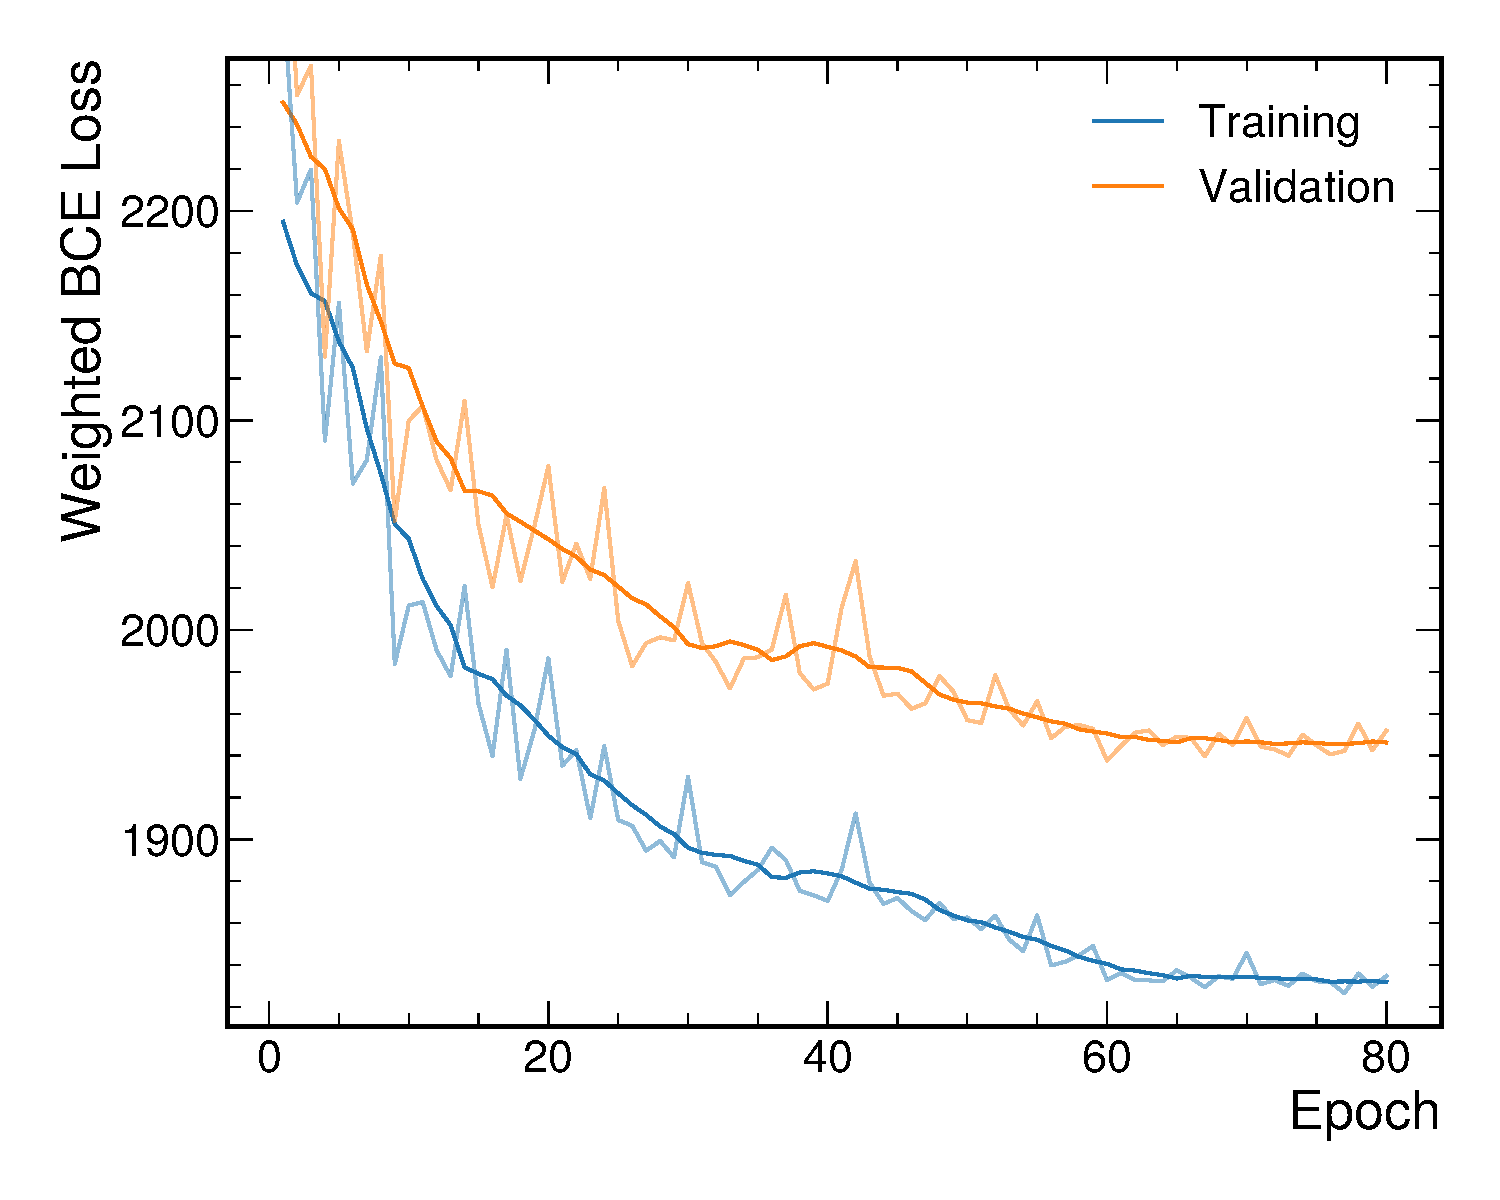
\includegraphics[width=0.49\textwidth]{Figures/Dihiggs/categorisation/y_tautau_loss.pdf} \\
    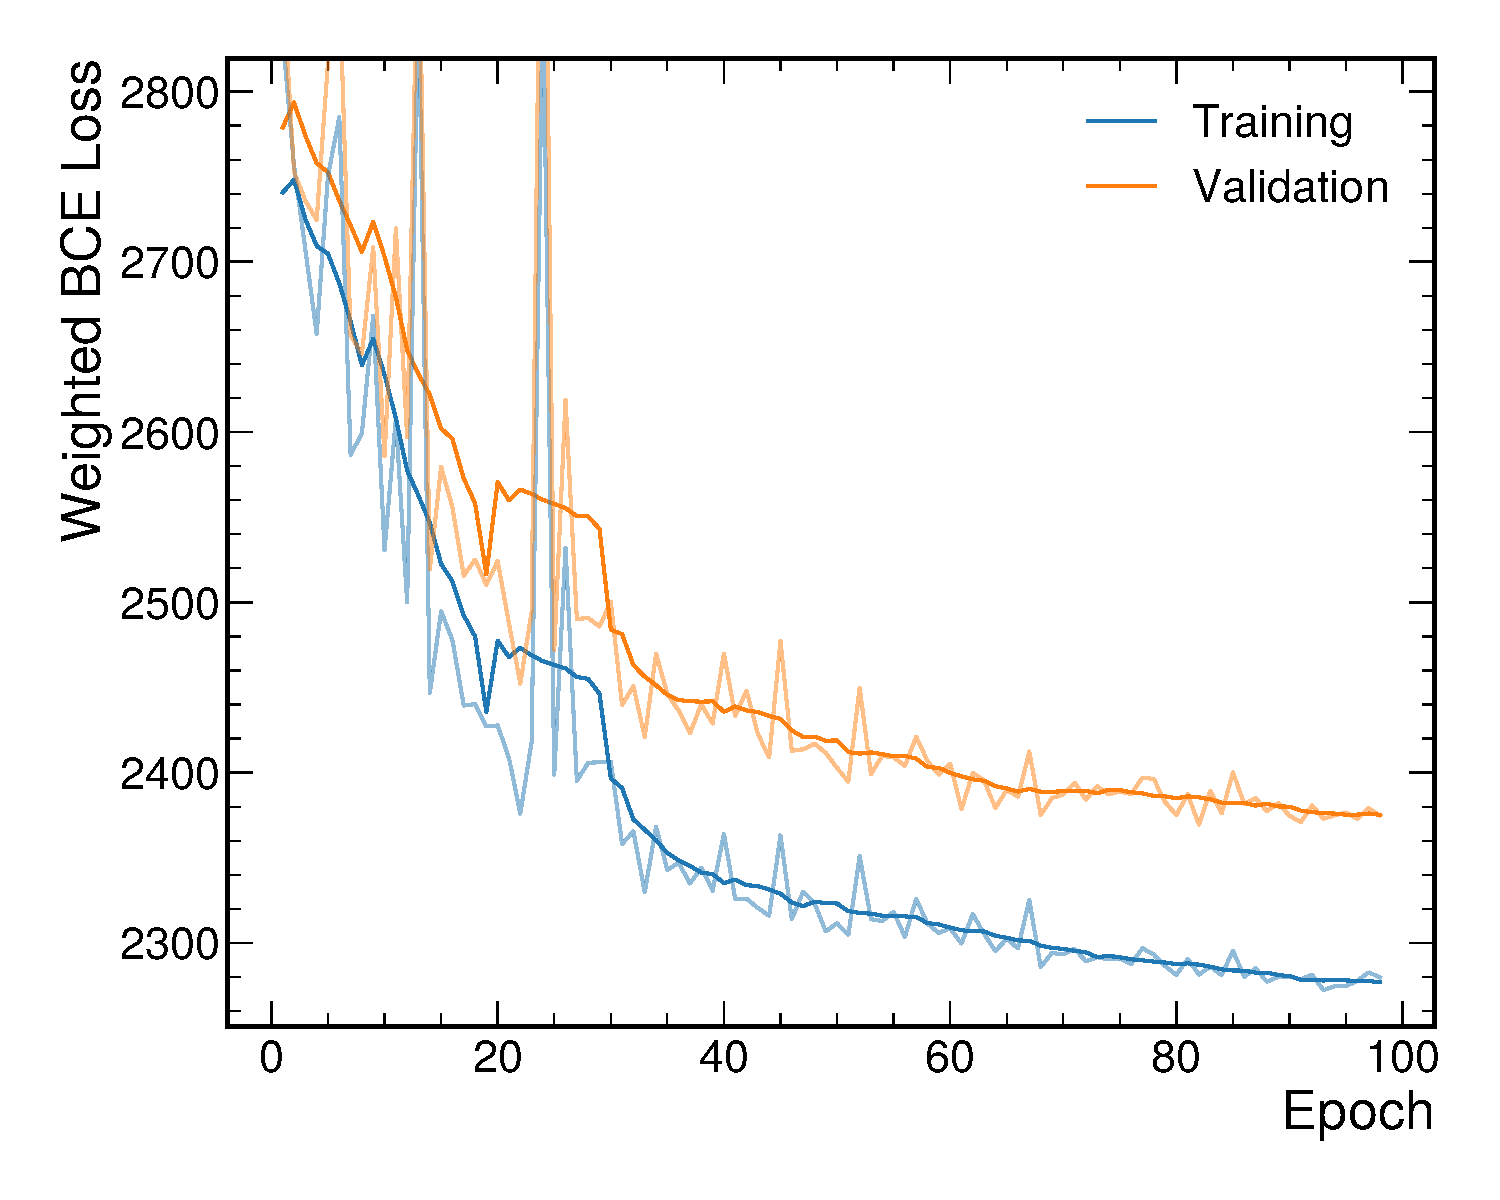
\includegraphics[width=0.49\textwidth]{Figures/Dihiggs/categorisation/y_gg_low_mass_loss.pdf}
    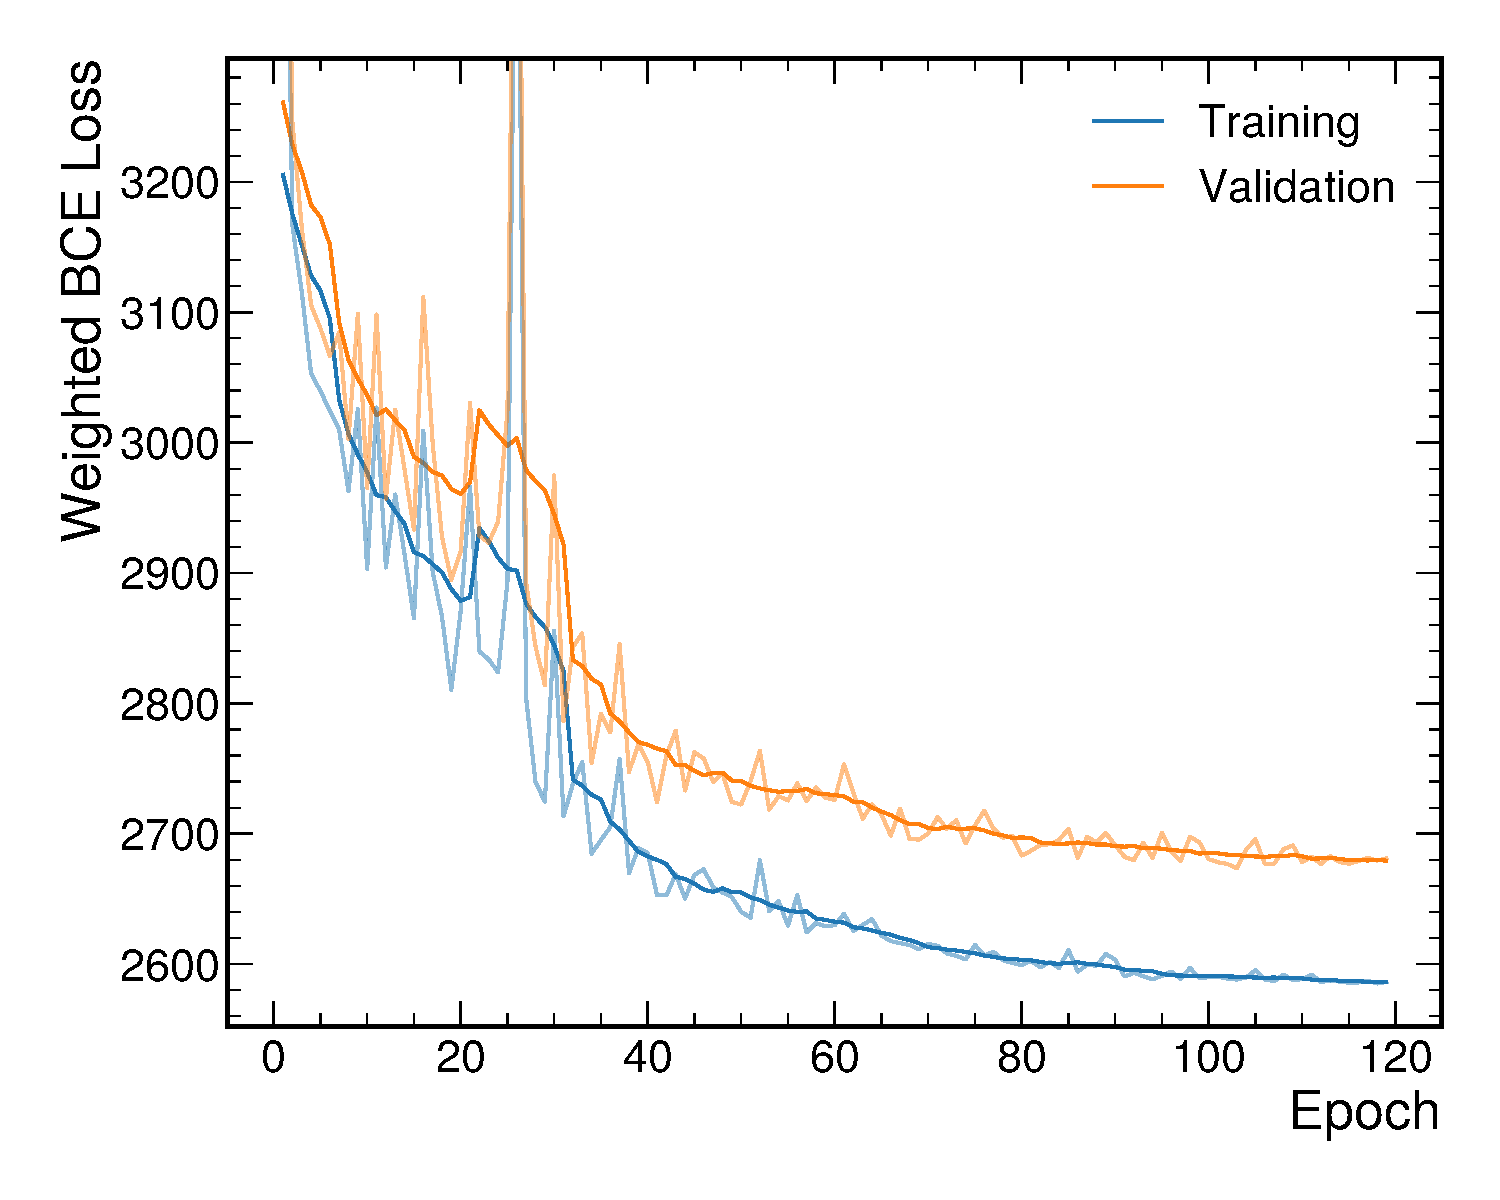
\includegraphics[width=0.49\textwidth]{Figures/Dihiggs/categorisation/y_gg_high_mass_loss.pdf}
    \caption[Evolution of BCE Loss for the \XZeroHH, and \XYH pNNs]{Total (not averaged) BCE loss for the \XZeroHH (top-left), \XYttHgg (top-right), low-mass \XYggHtt (bottom-left) and high-mass \XYggHtt (bottom-right) pNNs after every epoch of training for both the training and validation datasets. The total normalization of the dataset, and therefore, the scale of the loss, is arbitrary. The first loss values shown at Epoch 1 correspond to the losses after 1 epoch of training. The opaque lines represent a rolling average in a centred window of 10 epochs of the true loss values, shown by the faint lines of the same colour.}\label{fig:pNN_loss_rest}
\end{figure}

To test the pNN's performance, datasets are created for every mass hypothesis with simulated signal events corresponding to that hypothesis and simulated background events which include all processes described in \cref{sec:ggtt_samples}. These events are all taken from the testing dataset so that they are independent of the events used in training. In each dataset, the pNN is evaluated, setting the \mX and \mY (parametric) training features to the mass hypothesis of the dataset. Equivalent datasets are created using events from the training dataset to look for signs of overtraining.

In each dataset (mass hypothesis), the signal efficiency is calculated as a function of the background efficiency to create a receiver operating characteristic (ROC) curve, where these efficiencies are calculated with respect to the events that pass preselection. The area under the ROC curve (AUC) is then calculated to give a single number that represents the performance of the pNN for that mass hypothesis. For illustrative purposes, the ROC curves are plotted reversed in this section, i.e.\ background efficiency against signal efficiency. However, AUC scores still refer to the area under the ROC curve as it is normally defined, i.e.\ signal efficiency against background efficiency.  

ROC curves for the \XTwoHH pNN at $\mX=260$, 300, 500 and 1000\GeV are shown in \cref{fig:graviton_roc} and AUC scores for the rest of the mass hypotheses, and for the other searches are shown in \cref{fig:xhh_auc,fig:xyh_auc}. AUC scores for the testing dataset are in the range 0.9 to 0.9999 and are typically higher for signals with higher \mX and lower \mY, which correspond to processes with higher boosted \PH and \PY bosons.

In \cref{fig:graviton_roc,fig:xhh_auc}, the ROC curves and AUC scores are shown for the training dataset as well. The ROC curves for the \XTwoHH pNN are almost indistinguishable, especially for background efficiencies of $>1\%$ which is representative of the final categorization (see \cref{sec:cat_optim}). Similarly, small differences between the train and test AUC scores can be seen across the whole \mX range for \XTwoHH, and for the \XZeroHH pNN. This indicates that the pNNs have not been overtrained. This is also observed in the other searches. Regardless, only the events from the testing dataset are used for signal modelling to avoid any bias.

\begin{figure}
    \centering
    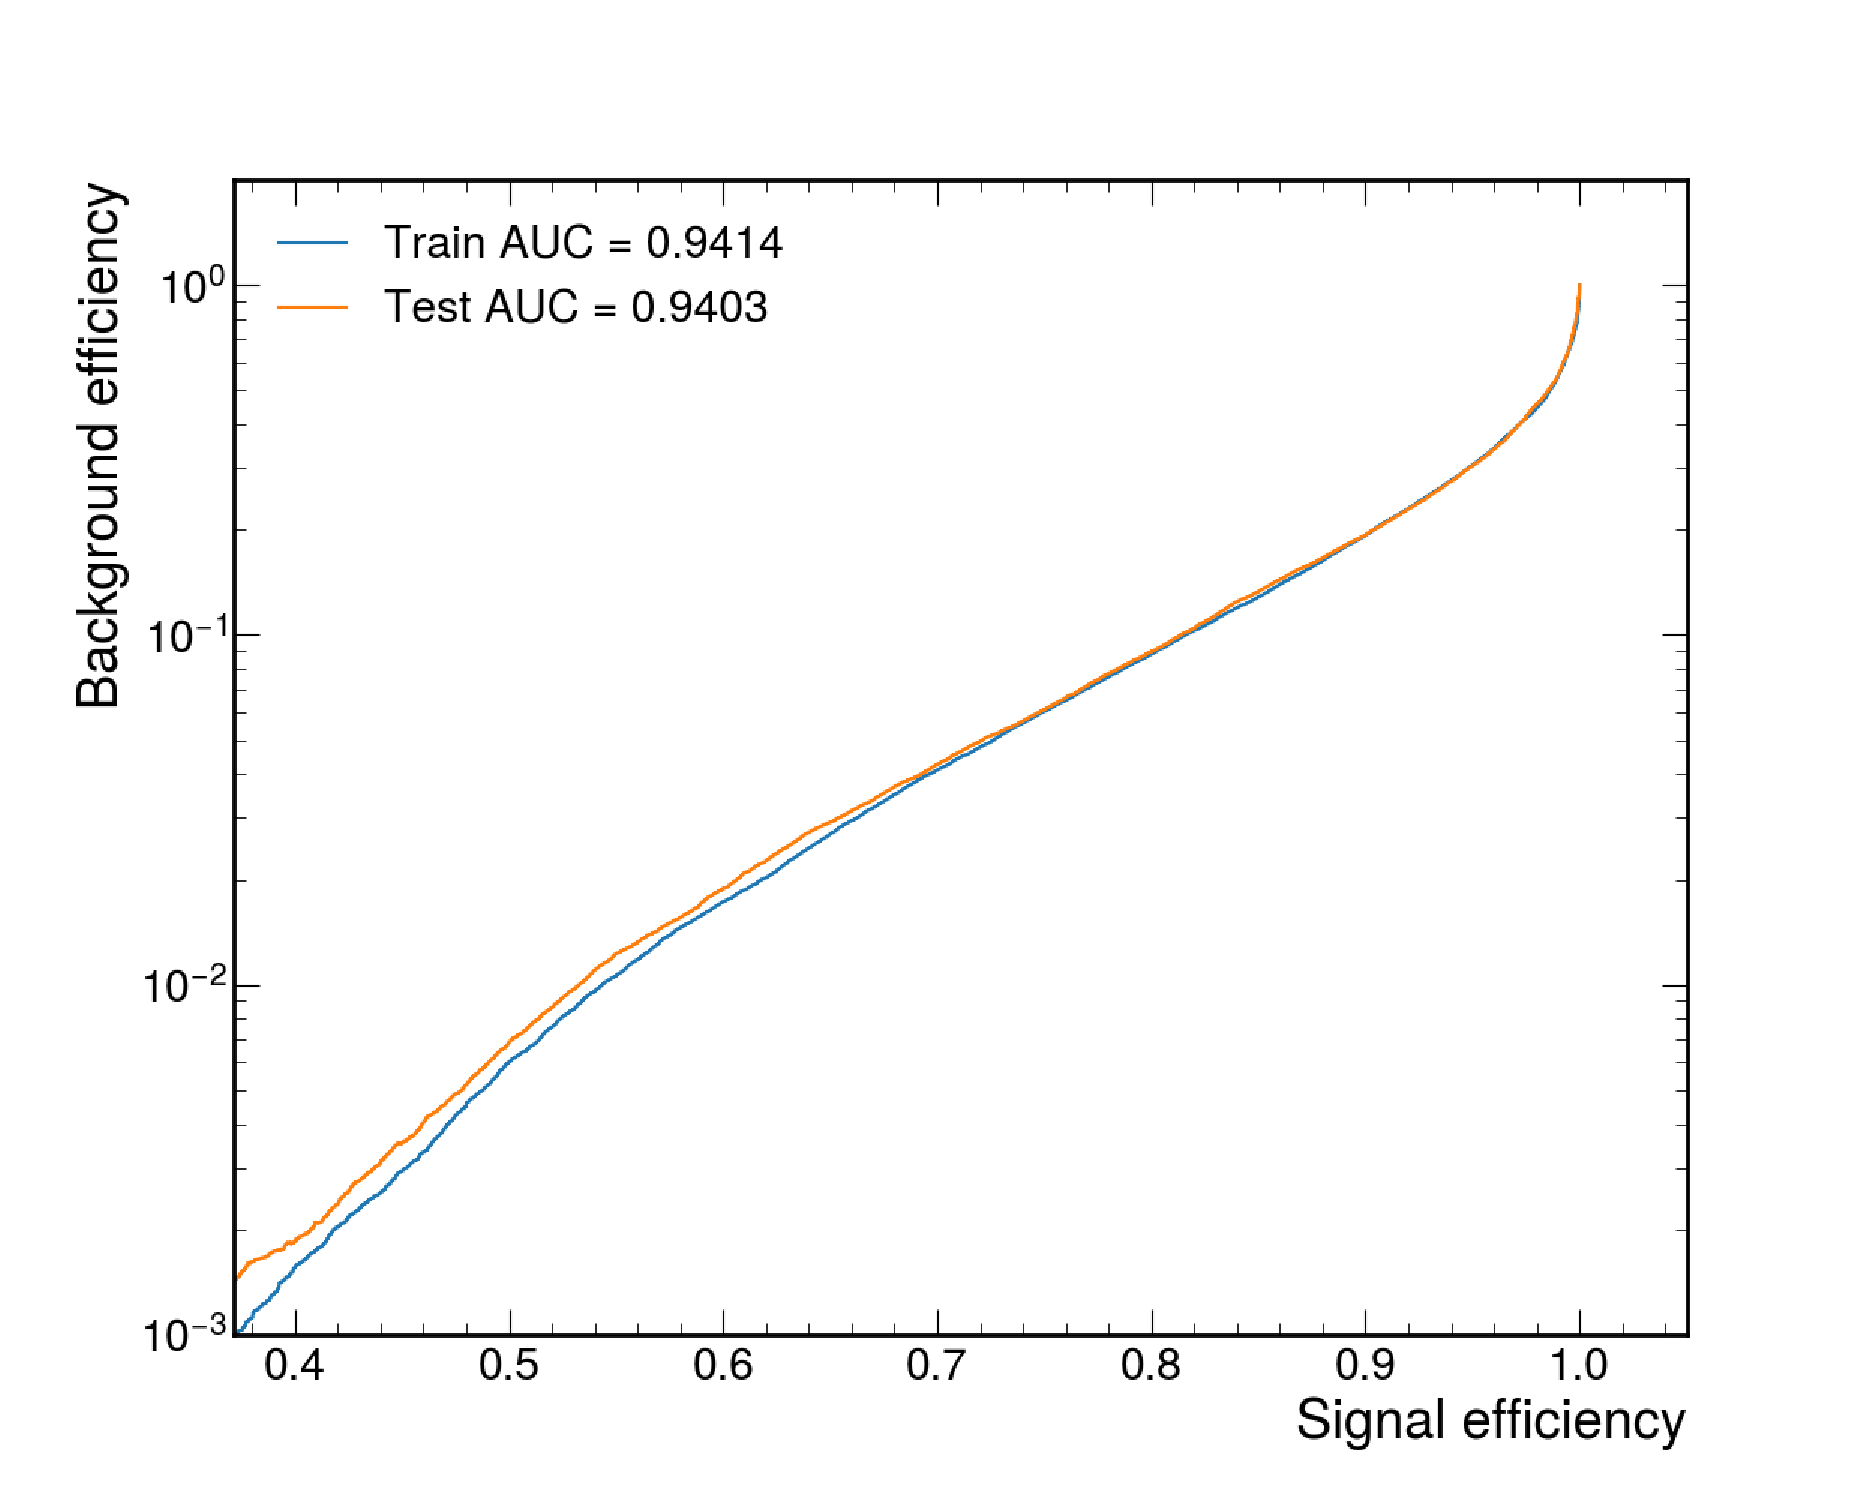
\includegraphics[width=0.49\textwidth]{Figures/Dihiggs/categorisation/ROC/Graviton/GluGluToBulkGravitonToHHTo2G2Tau_M-260/ROC_new.pdf}
    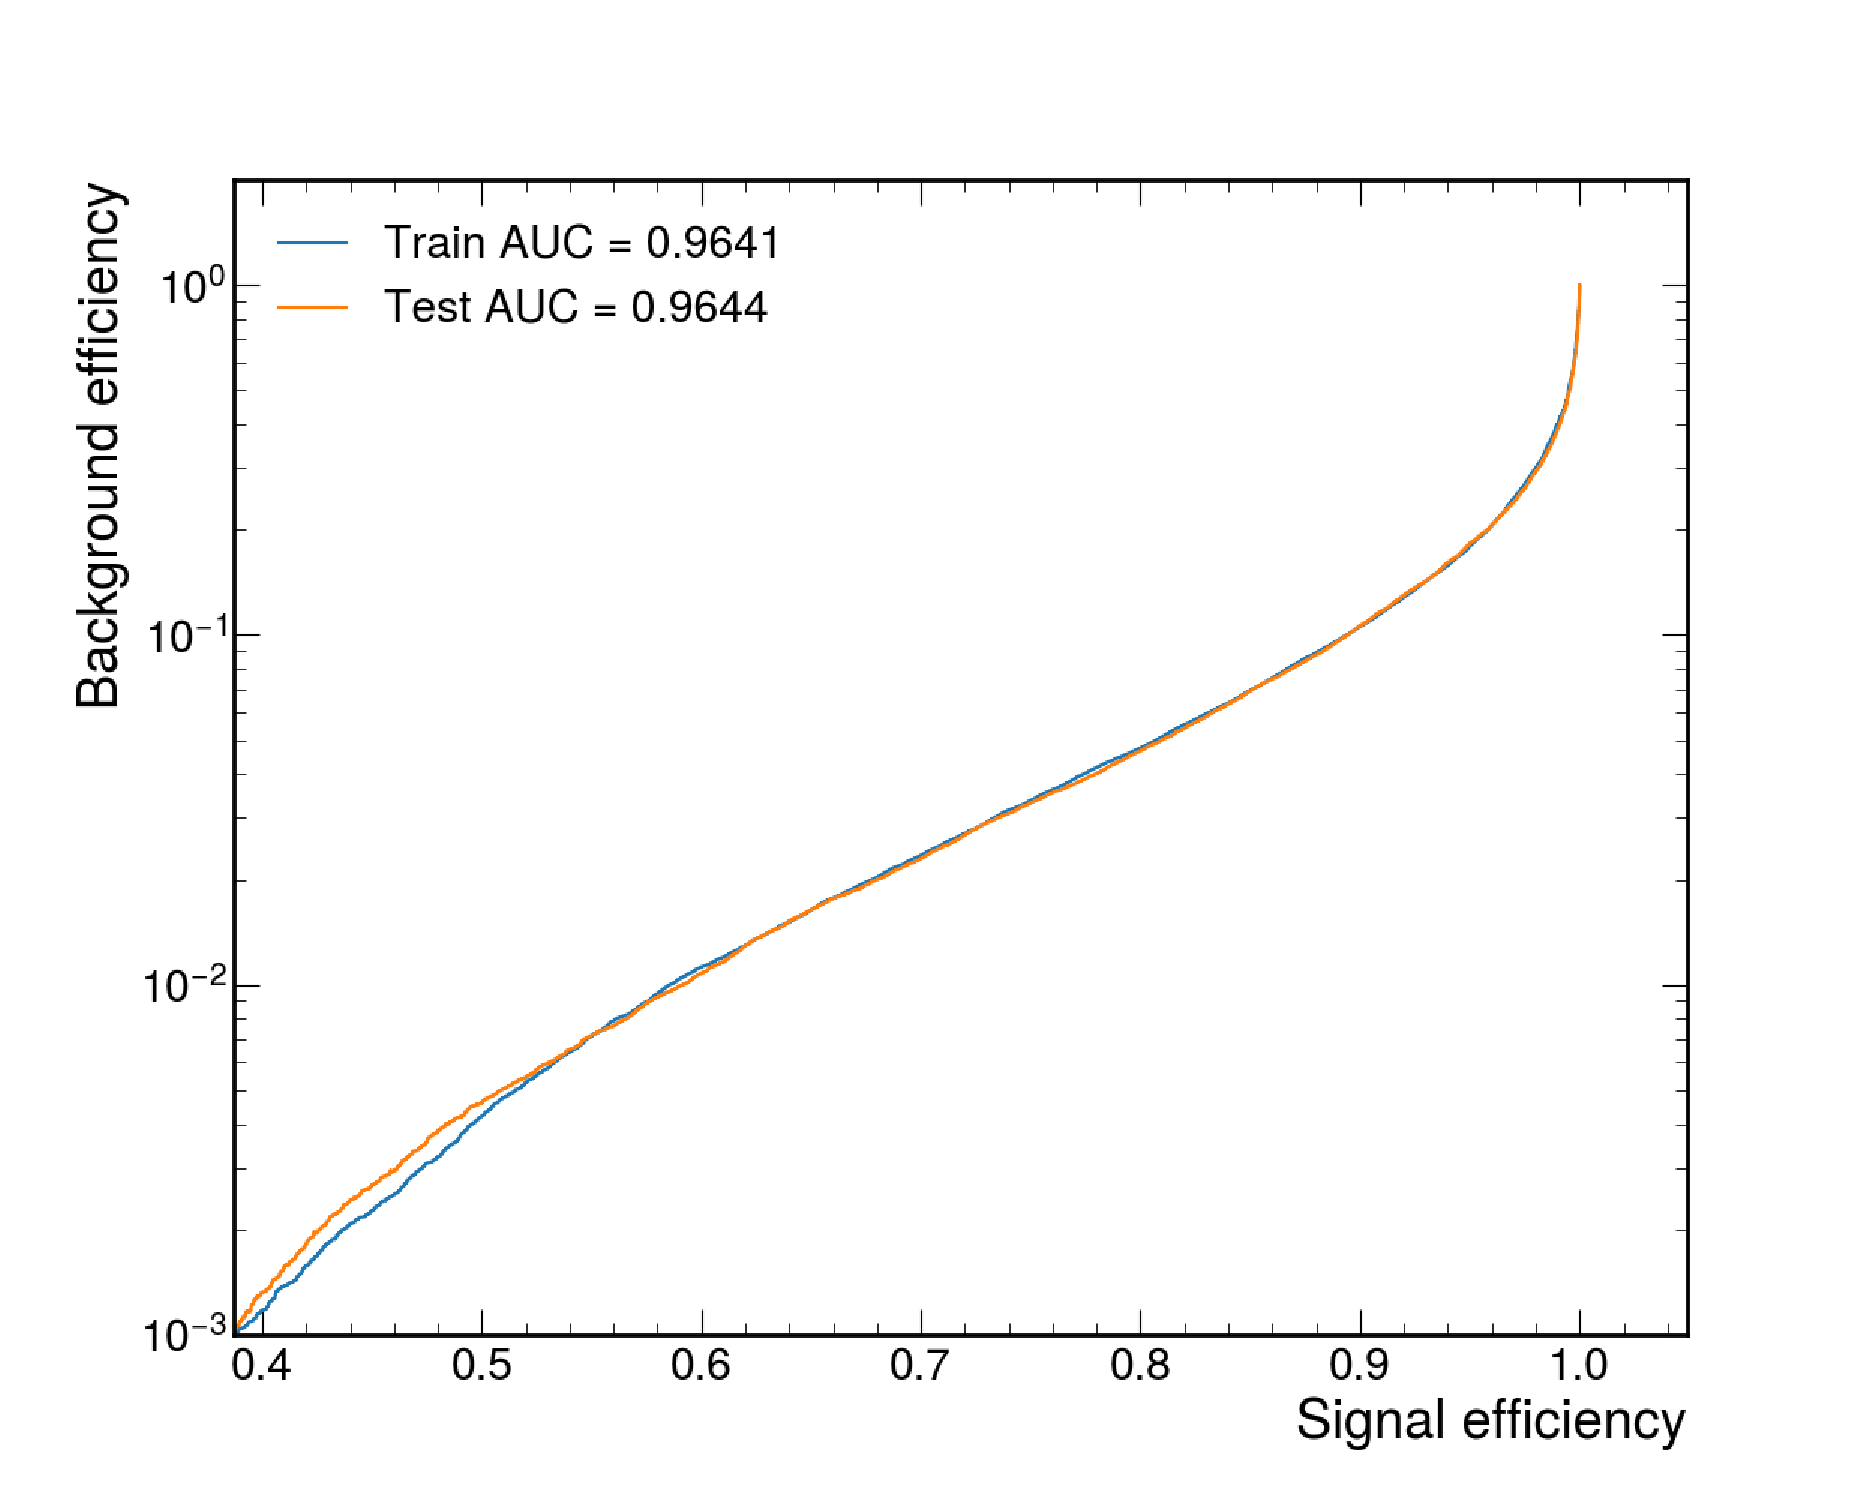
\includegraphics[width=0.49\textwidth]{Figures/Dihiggs/categorisation/ROC/Graviton/GluGluToBulkGravitonToHHTo2G2Tau_M-300/ROC_new.pdf} \\
    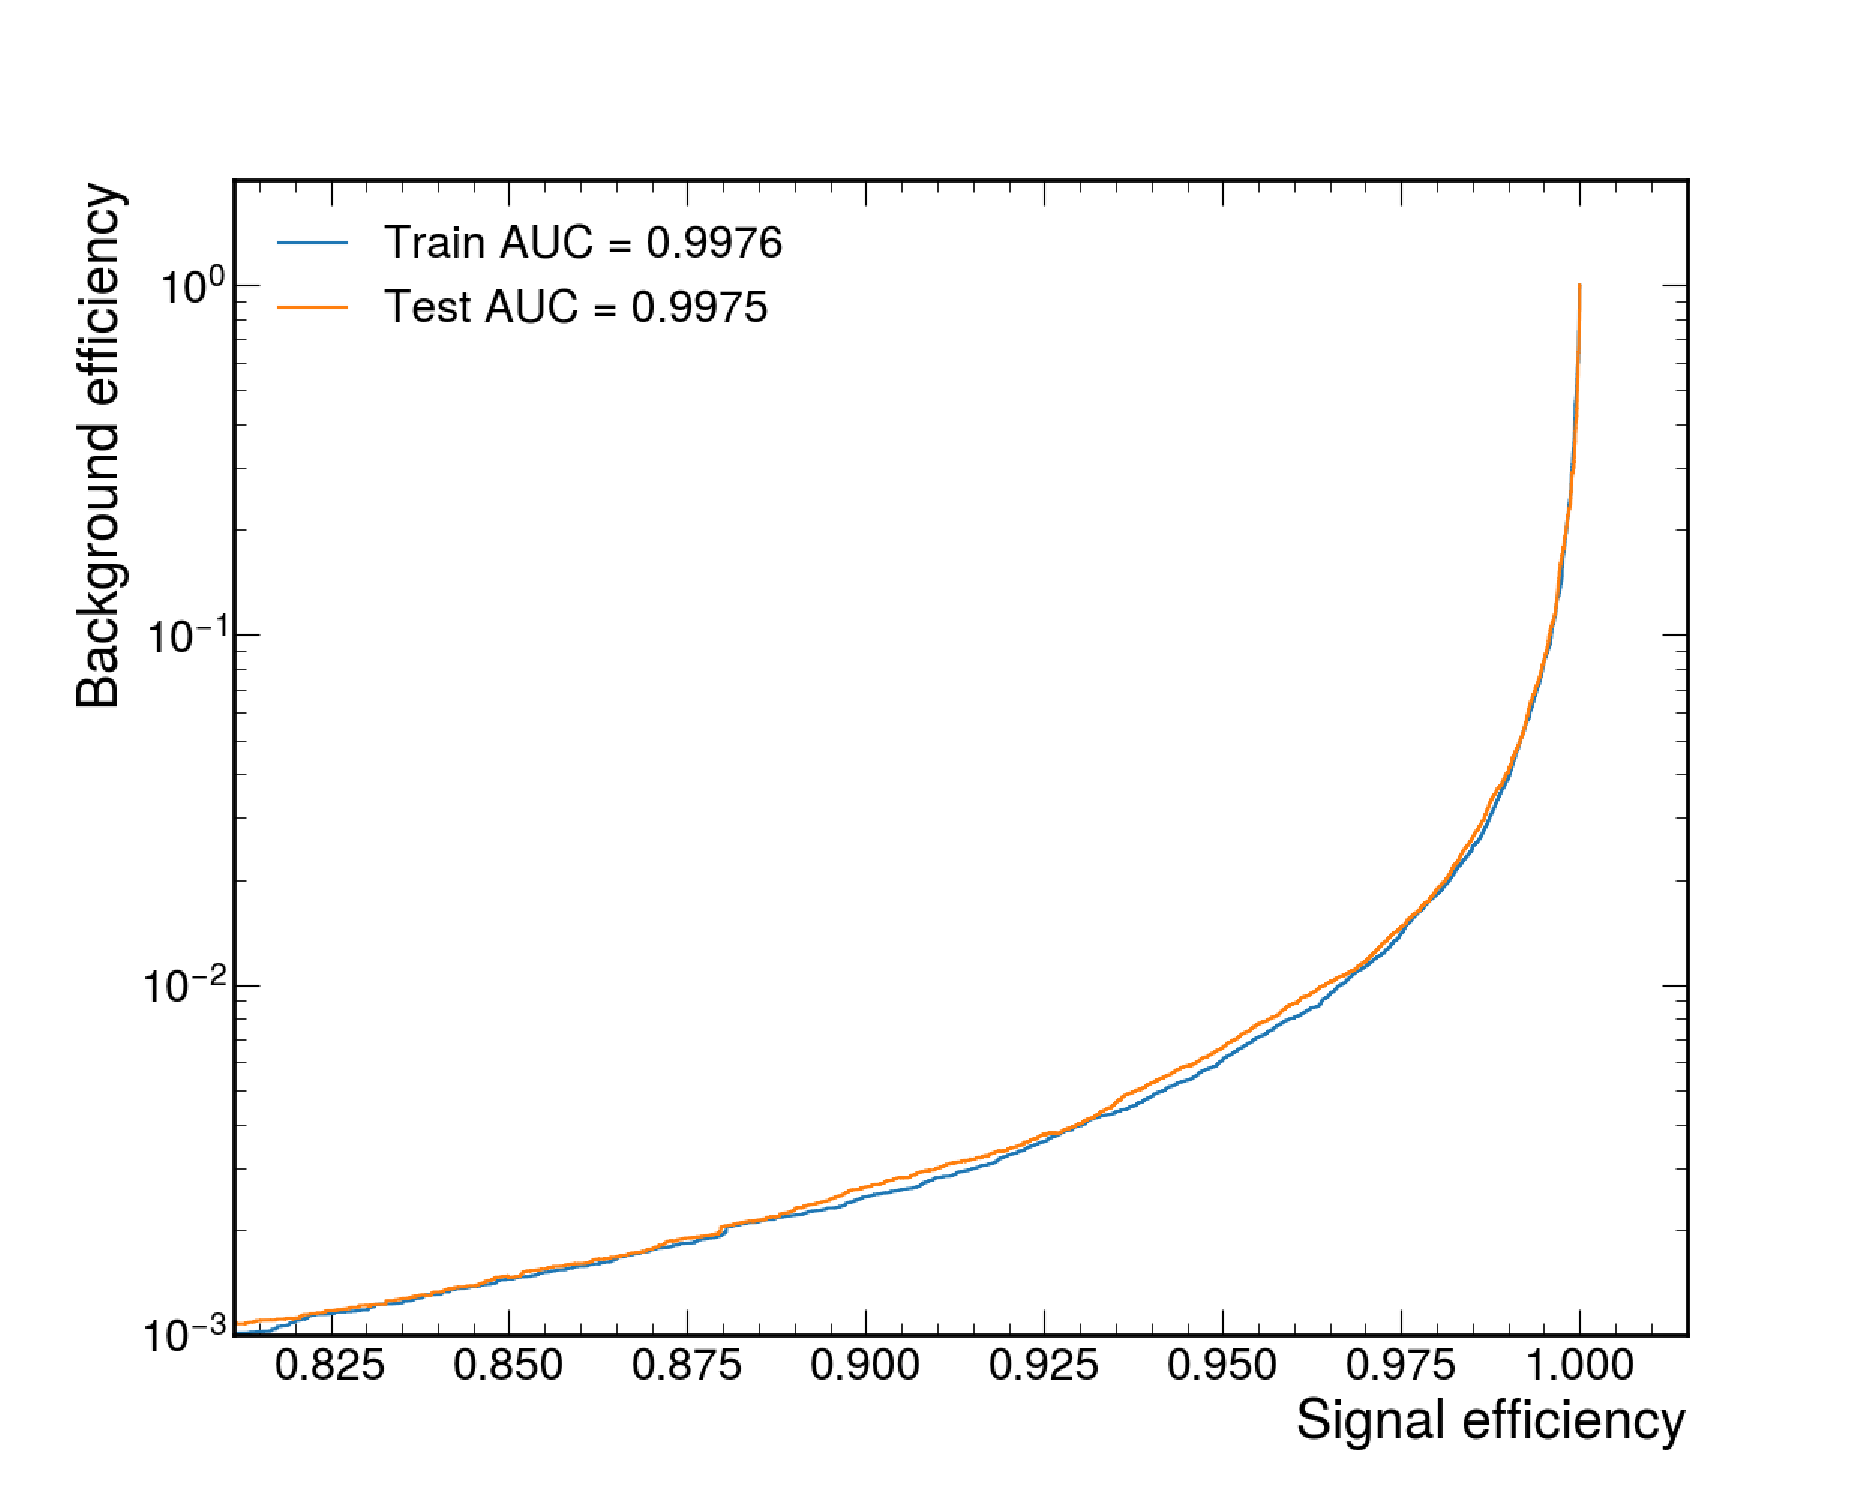
\includegraphics[width=0.49\textwidth]{Figures/Dihiggs/categorisation/ROC/Graviton/GluGluToBulkGravitonToHHTo2G2Tau_M-500/ROC_new.pdf}
    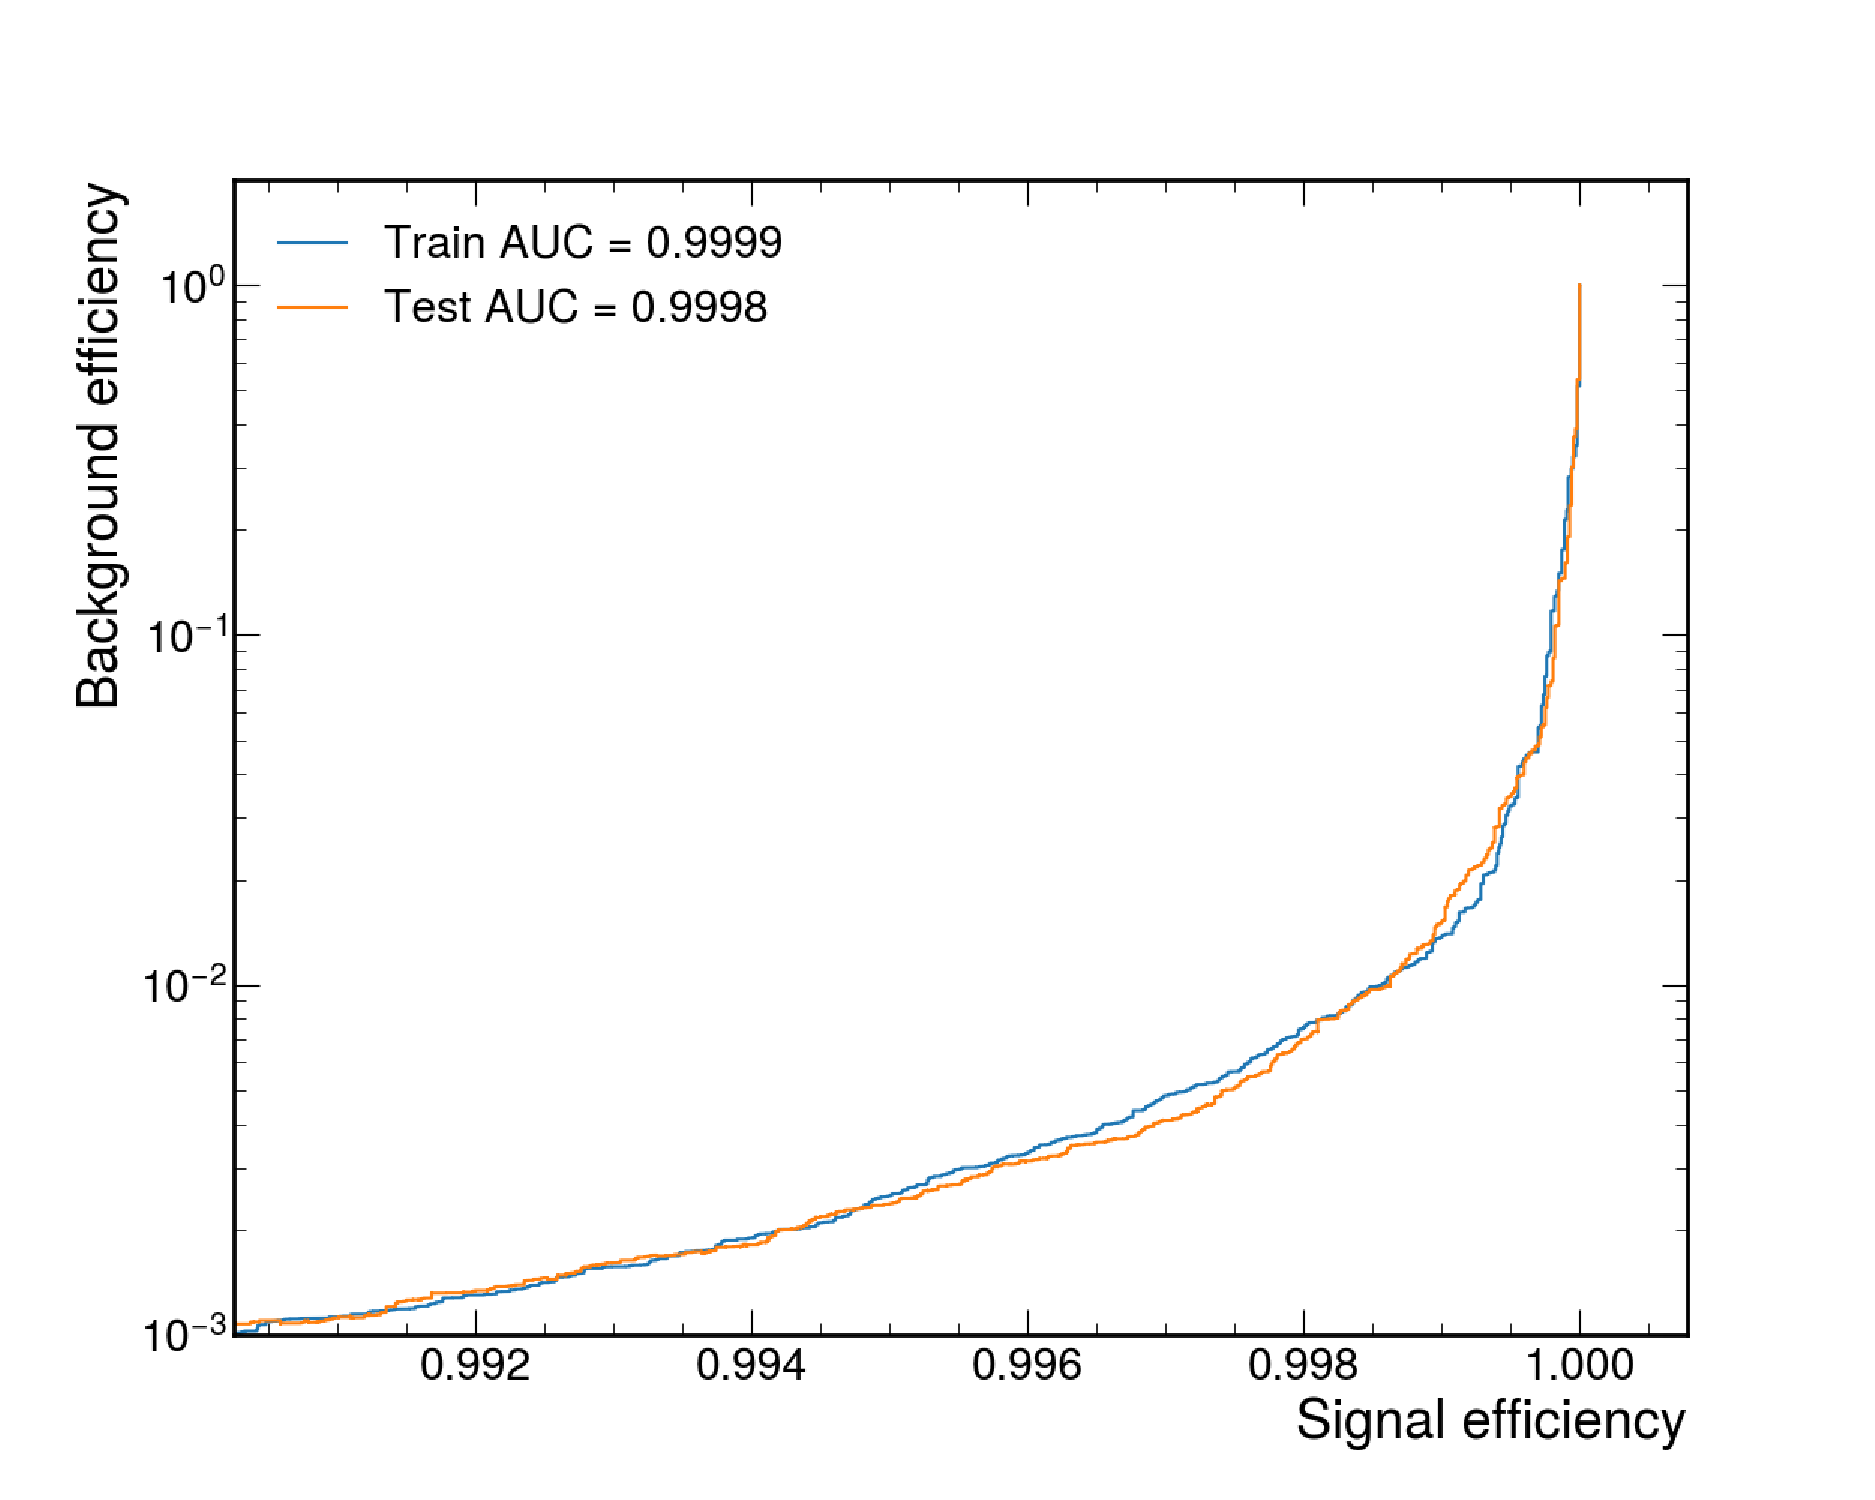
\includegraphics[width=0.49\textwidth]{Figures/Dihiggs/categorisation/ROC/Graviton/GluGluToBulkGravitonToHHTo2G2Tau_M-1000/ROC_new.pdf}
    \caption[ROC Curves for the \XTwoHH pNN]{ROC curves for the \XTwoHH pNN for $\mX=260$ (top-left), $\mX=300$ (top-right), $\mX=500$ (bottom-left) and $\mX=1000$\GeV (bottom-right). The curves are shown for the training and testing datasets. The efficiencies are calculated with respect to the events that pass preselection.}\label{fig:graviton_roc}
\end{figure}

\begin{figure}
    \centering
    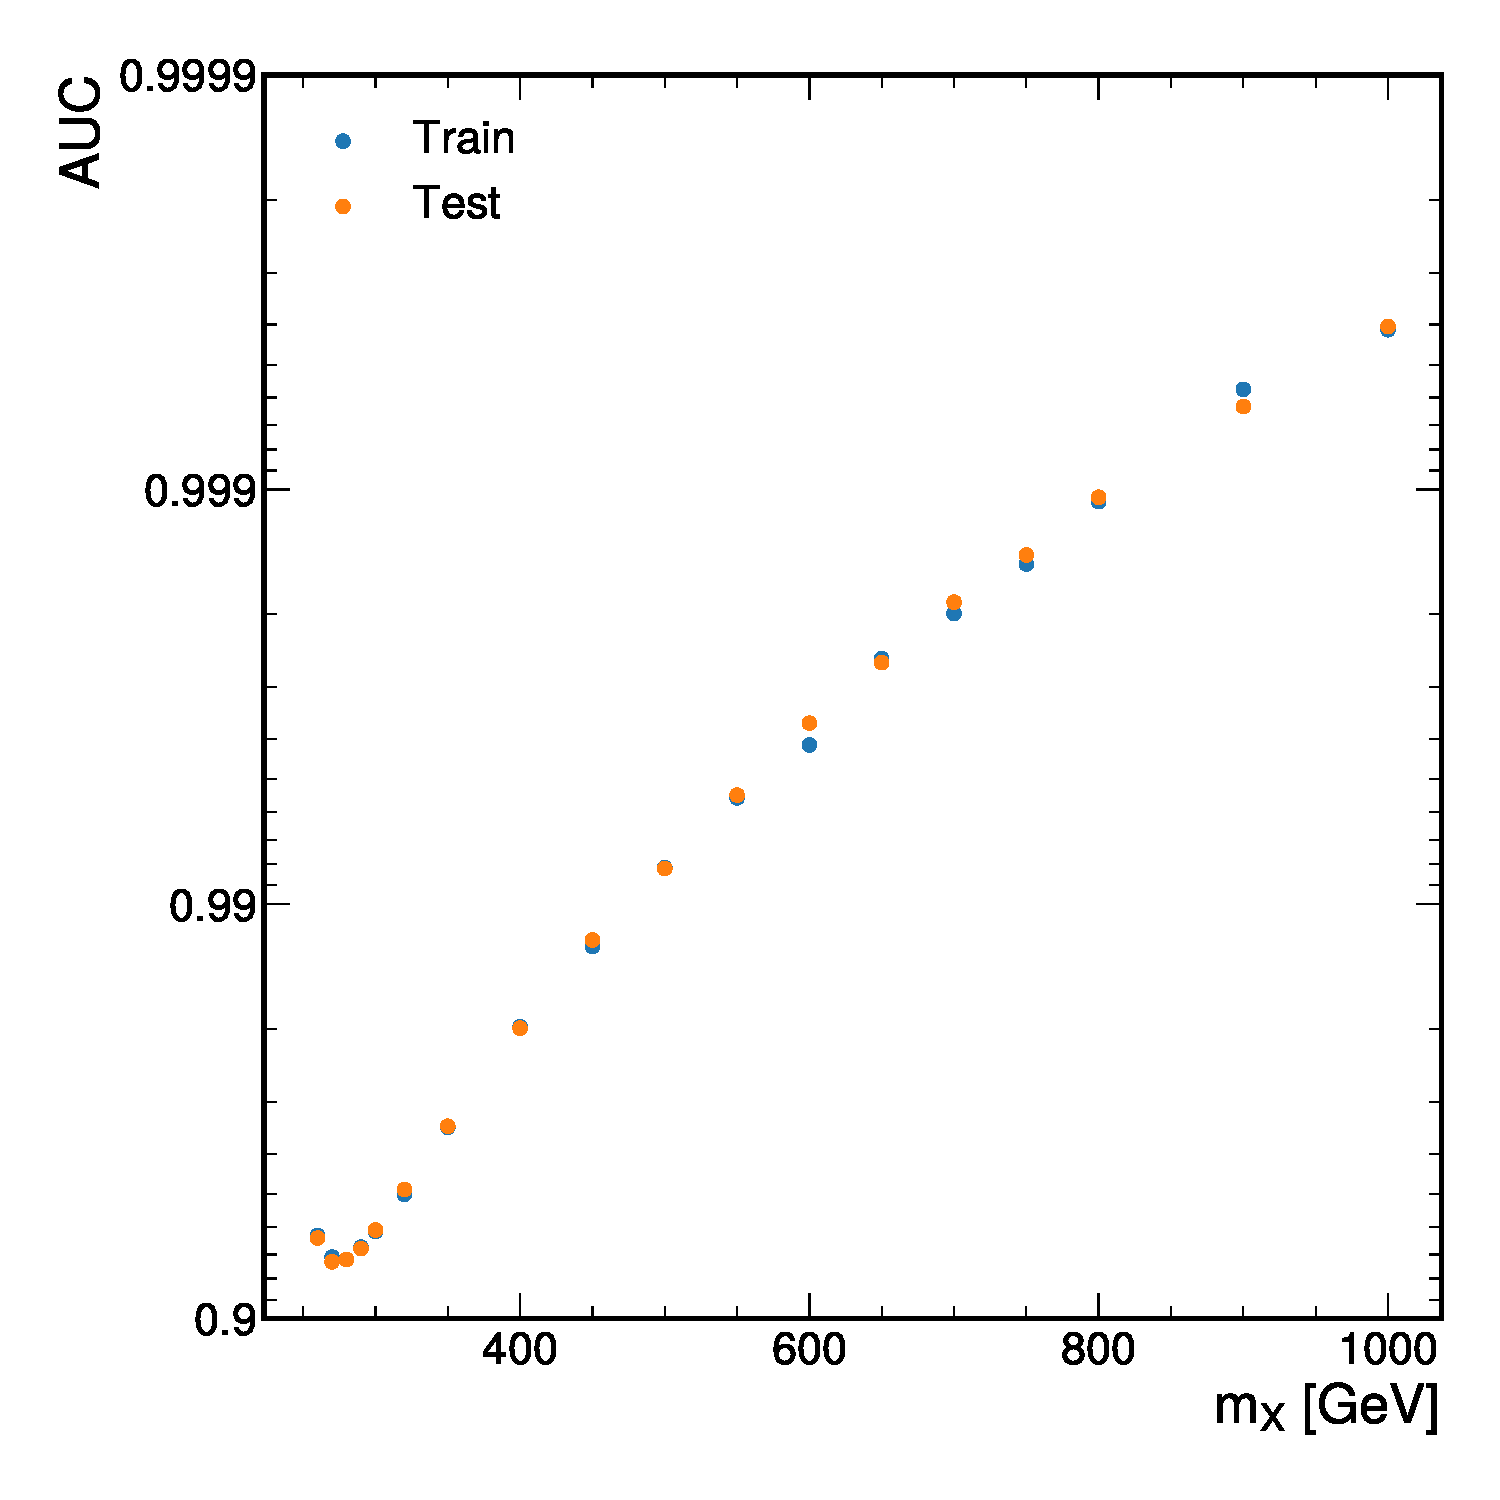
\includegraphics[width=0.49\textwidth]{Figures/Dihiggs/categorisation/ROC/Radion/auc.pdf}
    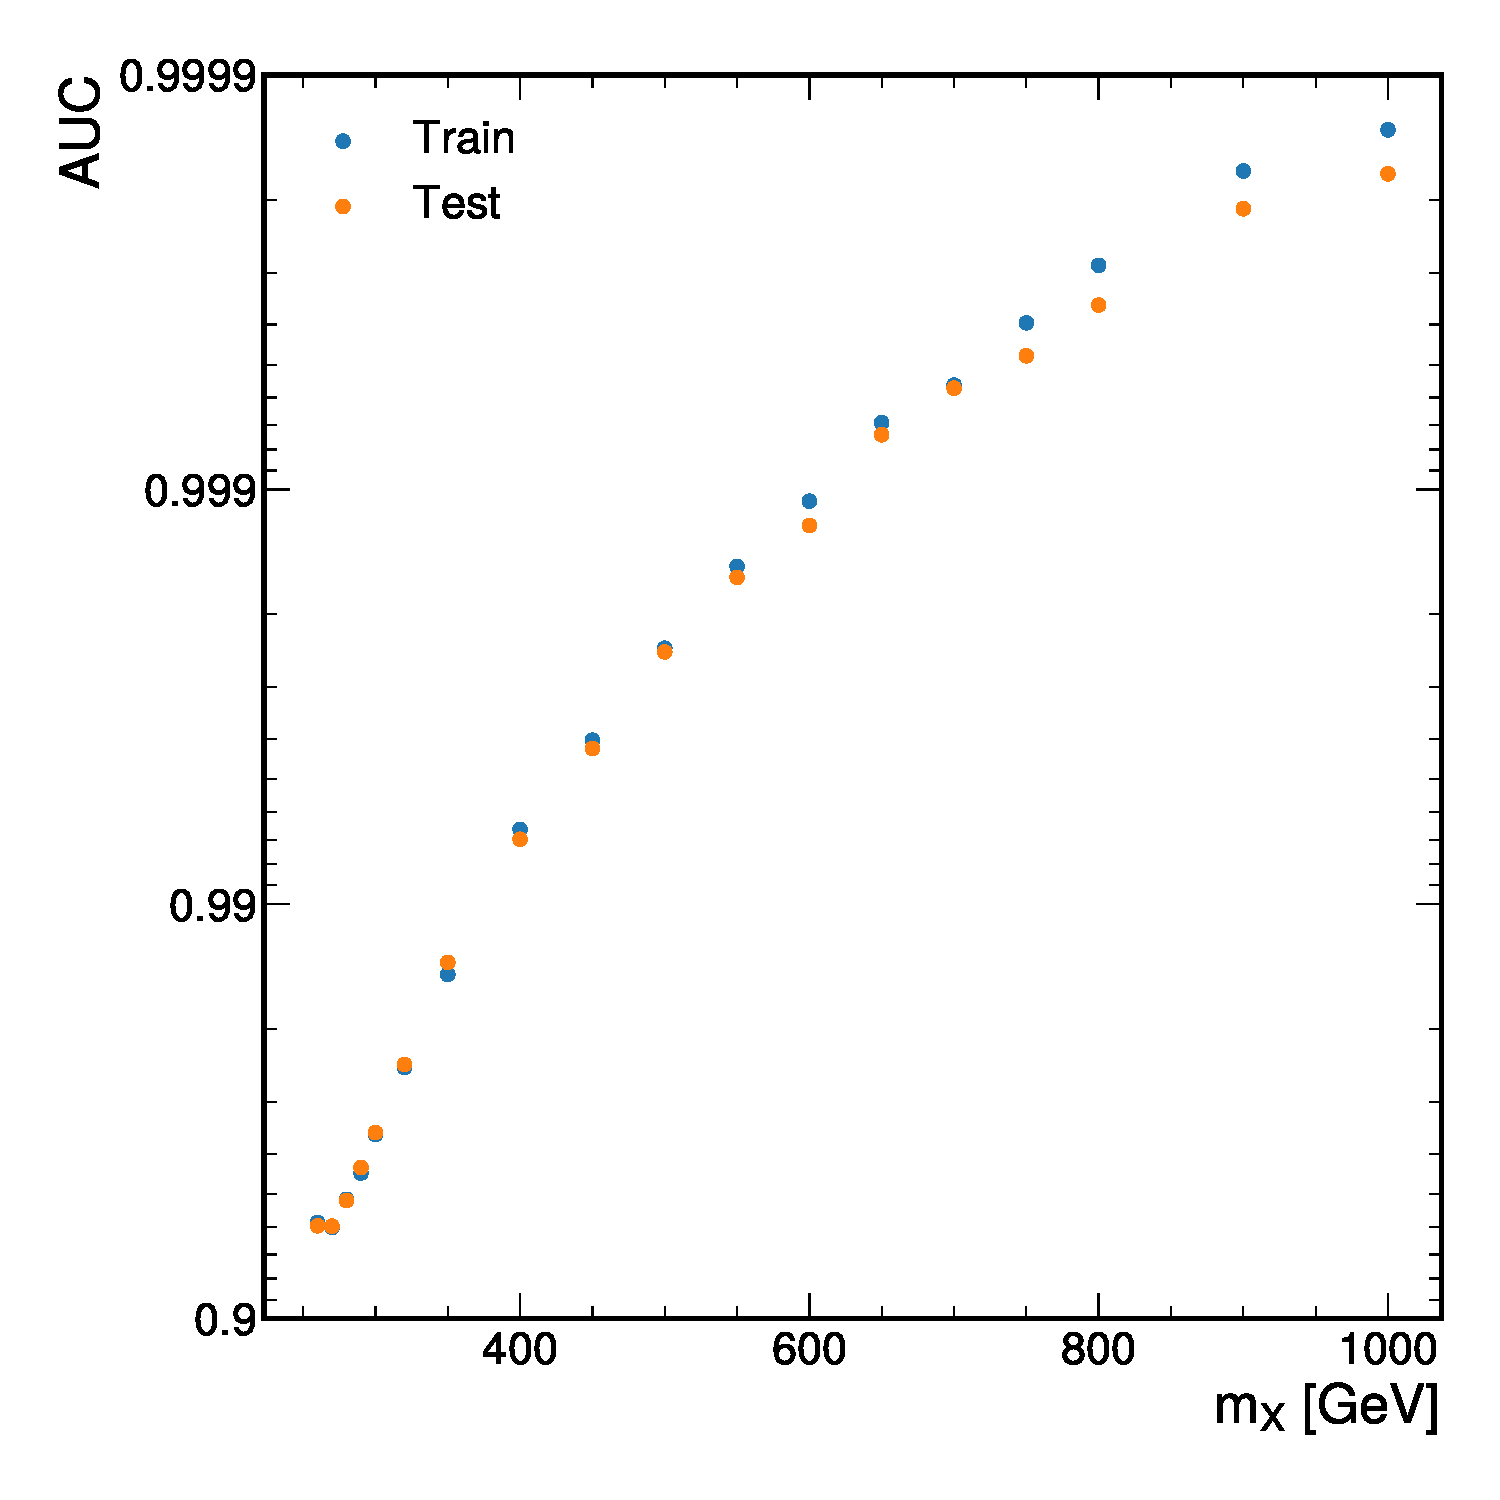
\includegraphics[width=0.49\textwidth]{Figures/Dihiggs/categorisation/ROC/Graviton/auc.pdf}
    \caption[AUC Scores for the \XHH pNNs]{AUC scores for the \XZeroHH (left) and \XTwoHH (right) pNNs for as a function of \mX. The scores are shown for the training and testing datasets. The signal and background efficiencies used to create the underlying ROC curves are calculated with respect to the events that pass preselection.}\label{fig:xhh_auc}
\end{figure}

\begin{figure}
    \centering
    \includegraphics[width=0.49\textwidth]{Figures/Dihiggs/categorisation/ROC/Y_tautau/auc.pdf} \\
    \includegraphics[width=0.49\textwidth]{Figures/Dihiggs/categorisation/ROC/Y_gg_Low_Mass/auc.pdf}
    \includegraphics[width=0.49\textwidth]{Figures/Dihiggs/categorisation/ROC/Y_gg_High_Mass/auc.pdf}
    \caption[AUC Scores for the \XYH pNNs]{AUC scores calculated on the testing datasets for the \XYttHgg (top), low-mass \XYggHtt (bottom-left), and high-mass \XYggHtt (bottom-right) pNNs as functions of \mX and \mY. The signal and background efficiencies used to create the underlying ROC curves are calculated with respect to the events that pass preselection.}\label{fig:xyh_auc}
\end{figure}

\newpage
In \cref{sec:pNN}, it was stated that the pNNs must fulfil two criteria to justify their use in this analysis: 1.\ there is good performance at every mass point, and 2.\ there is good performance at interpolated mass points. To study these criteria, the following tests are performed:
\begin{enumerate}
    \item Good performance at every mass point
    \begin{enumerate}
        \item Train a pNN using all of the mass points (`all' network)
        \item Train a separate NN for each mass point (`only' network)
        \item Compare the performance between (a) and (b) where the performance is evaluated on the (only) mass point that the NN was trained on
    \end{enumerate}
    \item Good performance at interpolated mass points
    \begin{enumerate}
        \item Train a pNN using all of the mass points (`all' network)
        \item Train a separate pNN on all mass points except one (`skip' network) 
        \item Compare the performance between (a) and (b) where the performance is evaluated on the excluded (skipped) mass point
    \end{enumerate}
\end{enumerate}
The performance metric used is the signal efficiency found at a background efficiency of 1\% which is representative of the final categorization in the analysis. In a search, the first test is performed at every mass point, and the second test is performed at every mass point except those at the boundaries of the mass ranges. This excludes scenarios where the pNN is asked to extrapolate to a mass point that is outside the range of masses used during training. The results of these tests are shown in \cref{fig:param_tests_graviton,fig:param_tests_low_mass,fig:param_tests_high_mass,fig:param_tests_y_tautau} for the \XTwoHH, \XYttHgg, low-mass \XYggHtt, and high-mass \XYggHtt pNNs respectively. The \XZeroHH pNN was not tested but is expected to perform similarly to the \XTwoHH pNN.

Across all searches, the majority of the tests show differences of less than 1\%. The `only' tests tend to show larger differences where the biggest differences are typically found at lower \mX and higher \mY, being up to 5\% and 2\% for the `only' and `skip' comparisons respectively. This trend in \mX and \mY is not entirely unexpected. As evident from the shape of the training features (\cref{sec:training_features}), the evolution of the loss for different masses (\cref{fig:pNN_loss_graviton}), and the AUC scores (\cref{fig:xhh_auc,fig:xyh_auc}), signals at lower \mX and higher \mY present a more complex discrimination problem. Therefore, it in unsurprising that dedicated networks (the `only' networks) show greater chances for improvement, and that it is more difficult to interpolate the behaviour of the network accurately. 

The majority of the tests show differences of less than 1\%, with a few losses up to 5\%. Given the benefits of using a pNN, the small number of larger losses are considered acceptable and pNNs are chosen as the final discriminators for the analysis. In future analyses, the losses could be minimized by splitting up the kinematic regime and training more specialized networks, or by investigating more complex architectures for the pNN.

\begin{figure}
    \centering
    \includegraphics[width=0.7\textwidth]{Figures/Dihiggs/categorisation/param_tests/Graviton/all_only.pdf} \\
    \includegraphics[width=0.7\textwidth]{Figures/Dihiggs/categorisation/param_tests/Graviton/all_skip.pdf}
    \caption[pNN Validation Tests in the \XTwoHH Search]{For the \XTwoHH search, results from the tests designed to check whether the pNN performs well at every mass point (top) and at interpolated mass points (bottom). Signal efficiencies correspond to a background efficiency of 1\%. The `all' efficiencies correspond to a pNN trained on all mass points. The `only' efficiencies correspond to a NN trained only on the mass point which the efficiency is quoted for. The `skip' efficiencies correspond to a pNN trained on all mass points except for the mass point where the efficiency is quoted for. The grey dashed lines in the bottom half of each plot correspond to differences of 1\%.}\label{fig:param_tests_graviton}
\end{figure}

\begin{figure}
    \centering
    \makebox[\textwidth][c]{\includegraphics[width=1.2\textwidth]{Figures/Dihiggs/categorisation/param_tests/NMSSM_Y_tautau/all_only.pdf}}
     \\
    \makebox[\textwidth][c]{\includegraphics[width=1.2\textwidth]{Figures/Dihiggs/categorisation/param_tests/NMSSM_Y_tautau/all_skip.pdf}}
    \caption[pNN Validation Tests in the \XYttHgg Search]{For the \XYttHgg search, results from the tests designed to check whether the pNN performs well at every mass point (top) and at interpolated mass points (bottom). Signal efficiencies correspond to a background efficiency of 1\%. The `all' efficiencies correspond to a pNN trained on all mass points. The `only' efficiencies correspond to a NN trained only on the mass point which the efficiency is quoted for. The `skip' efficiencies correspond to a pNN trained on all mass points except for the mass point where the efficiency is quoted for. The grey dashed lines in the bottom half of each plot correspond to differences of 1\%.}\label{fig:param_tests_y_tautau}
\end{figure}

\begin{figure}
    \centering
    \makebox[\textwidth][c]{\includegraphics[width=1.2\textwidth]{Figures/Dihiggs/categorisation/param_tests/NMSSM_Y_gg_Low_Mass/all_only.pdf}}
     \\
    \makebox[\textwidth][c]{\includegraphics[width=1.2\textwidth]{Figures/Dihiggs/categorisation/param_tests/NMSSM_Y_gg_Low_Mass/all_skip.pdf}}
    \caption[pNN Validation Tests in the Low-Mass \XYggHtt Search]{For the low-mass \XYggHtt search, results from the tests designed to check whether the pNN performs well at every mass point (top) and at interpolated mass points (bottom). Signal efficiencies correspond to a background efficiency of 1\%. The `all' efficiencies correspond to a pNN trained on all mass points. The `only' efficiencies correspond to a NN trained only on the mass point which the efficiency is quoted for. The `skip' efficiencies correspond to a pNN trained on all mass points except for the mass point where the efficiency is quoted for. The grey dashed lines in the bottom half of each plot correspond to differences of 1\%.}\label{fig:param_tests_low_mass}
\end{figure}

\begin{figure}
    \centering
    \makebox[\textwidth][c]{\includegraphics[width=1.2\textwidth]{Figures/Dihiggs/categorisation/param_tests/NMSSM_Y_gg_High_Mass/all_only.pdf}} \\
    \makebox[\textwidth][c]{\includegraphics[width=1.2\textwidth]{Figures/Dihiggs/categorisation/param_tests/NMSSM_Y_gg_High_Mass/all_skip.pdf}}
    \caption[pNN Validation Tests in the High-Mass \XYggHtt Search]{For the high-mass \XYggHtt search, results from the tests designed to check whether the pNN performs well at every mass point (top) and at interpolated mass points (bottom). Signal efficiencies correspond to a background efficiency of 1\%. The `all' efficiencies correspond to a pNN trained on all mass points. The `only' efficiencies correspond to a NN trained only on the mass point which the efficiency is quoted for. The `skip' efficiencies correspond to a pNN trained on all mass points except for the mass point where the efficiency is quoted for. The grey dashed lines in the bottom half of each plot correspond to differences of 1\%.}\label{fig:param_tests_high_mass}
\end{figure}

\subsection{Category Optimization}\label{sec:cat_optim}

For a pair of masses, $(\mX,\mY) = (\mX^i, \mY^j)$, a set of analysis categories are defined based upon $f(\vec{x}; \mX=m^i, \mY=m^j)$, where $f(\vec{x}; \mX, \mY)$ is the pNN output score. Before defining these categories, the raw output score from the network is transformed such that the background MC from the test dataset is flat in the transformed score. The transformed score is denoted $\tilde{f}(\vec{x}; \mX, \mY)$. Like in training, the $\gamma + \text{jets}$ and $t\bar{t} + \text{jets}$ datasets are not used for the transformation. This transformation is motivated by the interpolation that is necessary to create signal models for the intermediate mass points. When placing a cut on $\tilde{f}(\vec{x}; \mX, \mY)$, it is equivalent to placing a cut on the \textit{training} background efficiency, and at a fixed background efficiency, the signal efficiency is expected to be a smooth function of \mX and \mY. \cref{fig:xhh_auc,fig:xyh_auc,fig:param_tests_graviton,fig:param_tests_y_tautau,fig:param_tests_low_mass,fig:param_tests_high_mass} already suggest that this is indeed the case. 

Distributions of the transformed output score for a selection of mass points are shown for the \XHH and \XYH searches in \cref{fig:pnn_xhh_evolution,fig:pnn_resonant}. The background distributions are almost flat, but not exactly since the $\gamma + \text{jets}$ and $t\bar{t} + \text{jets}$ datasets, which are not in the transformation, are included in these plots. The signal distributions peak sharply at $\tilde{f}(\vec{x}; \mX, \mY)=1$, meaning that the optimized categories can be expected to be defined at high values of $\tilde{f}(\vec{x}; \mX, \mY)$.

\begin{figure}
    \centering
    \includegraphics[width=.49\textwidth]{Figures/Dihiggs/categorisation/intermediate_transformed_score_GluGluToBulkGravitonToHHTo2G2Tau_M-260_GluGluToBulkGravitonToHHTo2G2Tau_M-260_paper.pdf}
    \includegraphics[width=.49\textwidth]{Figures/Dihiggs/categorisation/intermediate_transformed_score_GluGluToBulkGravitonToHHTo2G2Tau_M-800_GluGluToBulkGravitonToHHTo2G2Tau_M-800_paper.pdf}
    \caption[Transformed pNN Output Score Distribution in \XTwoHH Search]{Transformed pNN output distribution in the \XTwoHH search, evaluated at $\mX=260\GeV$ (left) and $\mX=800\GeV$ (right). The filled histograms represent the background simulation, and the corresponding statistical uncertainty is shown by the grey bands. The data are shown by black points, and the signal is shown by a black line. The background MC simulation is normalized to data and the signal is normalized to an arbitrary cross section for representation purposes.}\label{fig:pnn_xhh_evolution}
\end{figure}

\begin{figure}
    \centering
    \includegraphics[width=.49\textwidth]{Figures/Dihiggs/categorisation/intermediate_transformed_score_GluGluToRadionToHHTo2G2Tau_M-350_GluGluToRadionToHHTo2G2Tau_M-350_paper.pdf}
    \includegraphics[width=.49\textwidth]{Figures/Dihiggs/categorisation/intermediate_transformed_score_GluGluToBulkGravitonToHHTo2G2Tau_M-400_GluGluToBulkGravitonToHHTo2G2Tau_M-400_paper.pdf}
    \includegraphics[width=.49\textwidth]{Figures/Dihiggs/categorisation/intermediate_transformed_score_NMSSM_XYH_Y_tautau_H_gg_MX_300_MY_70_NMSSM_XYH_Y_tautau_H_gg_MX_300_MY_70_paper.pdf}
    \\
    \includegraphics[width=.49\textwidth]{Figures/Dihiggs/categorisation/intermediate_transformed_score_NMSSM_XYH_Y_gg_H_tautau_MX_500_MY_125_NMSSM_XYH_Y_gg_H_tautau_MX_500_MY_125_paper.pdf}
    \includegraphics[width=.49\textwidth]{Figures/Dihiggs/categorisation/intermediate_transformed_score_NMSSM_XYH_Y_gg_H_tautau_MX_500_MY_150_NMSSM_XYH_Y_gg_H_tautau_MX_500_MY_150_paper.pdf}
    \caption[Transformed pNN Output Scores in the \XZeroHH and \XYH Searches]{Transformed pNN output distribution in the \XZeroHH (upper left), \XTwoHH (upper right), \XYttHgg (middle), low-mass \XYggHtt (lower left) and high-mass \XYggHtt (lower right) searches. The pNNs are evaluated at the mass points where the largest excess with respect to the background-only hypothesis is observed. The filled histograms represent the background simulation, and the corresponding statistical uncertainty is shown by the grey bands. The data are shown by black points, and the signal is shown by a black line. The background MC simulation is normalized to data and the signal is normalized to an arbitrary cross section for representation purposes.}\label{fig:pnn_resonant}
\end{figure}

To optimize the category boundaries, a metric for the performance of a set of boundaries must be chosen. Given that the normalization of the signal is not known a priori, a metric independent of the normalization is desired, and here, the expected upper limit at the 95\% CL is used. The procedure used to calculate this limit is a simplified and computationally faster version of the final procedure used in the analysis. For a given nominal mass point, the upper limit is calculated as follows:
\begin{enumerate}
    \item In each analysis category:
    \begin{enumerate}
        \item Fit an exponential function to the $\mgg$ distribution in the nonresonant MC samples.
        \item Define a signal region as the $\pm1\sigma$ window centred around $\hat{m}_{\gamma\gamma}$, where $\sigma$ and $\hat{m}_{\gamma\gamma}$ are the standard deviation and mean values respectively of \mgg in the signal MC events.
        \item Determine the expected number of background events in the signal region by integrating the fitted exponential over that range.
        \item Determine the expected number of signal events in the signal region by summing the weights of the signal MC events that in the region.
    \end{enumerate}
    \item Use the expected number of signal and background events in the signal regions to perform a counting experiment and determine the upper limit according to the techniques described in \cref{chap:stats} using an asymptotic approximation for the distribution of the test statistic~\cite{Cowan:2010js}.
\end{enumerate}
The expected upper limit at an intermediate mass point cannot be determined in the same way because there is no signal MC for those points. The signal yields could instead be interpolated from those at the nominal mass points, but this would complicate the categorization optimization procedure. Instead, a procedure which used only the nominal mass points, but is still applicable, and optimal (or close to) at the intermediate mass points was devised.

At first, a categorization procedure was investigated where the same boundaries on $\tilde{f}(\vec{x}; \mX, \mY)$ were used for every mass point. This was tested on the \XTwoHH search, and the boundary values were determined by a grid search of 3 categories that optimized the expected limit at $\mX=280$\GeV. This strategy may bias itself towards the $\mX=280$\GeV mass point, so the resulting expected limits at other masses were compared to those found by performing the grid search at those masses instead. The comparison, shown in \cref{fig:cat_optimal_comparison}, finds up to 25\% differences in the expected upper limit and this was considered an unacceptable loss in sensitivity and therefore, alternative procedures were considered. 

\begin{figure}
    \centering
    \includegraphics[width=0.65\textwidth]{Figures/Dihiggs/categorisation/cat_optimal.pdf}
    \caption[Performance of a Grid Search of Category Boundaries at Every Mass Point Compared to a Single Point]{Comparison between the 95\% CL expected upper limit on $\sigma(\ppXHHggtt)$ reached when using the boundaries optimized for each mass point and when using the boundaries found for $\mX=280$\GeV for all mass points.}\label{fig:cat_optimal_comparison}
\end{figure}

During the grid search, it was imposed that the minimum number of expected background events be 10 in each category. This requirement is made to ensure a bias of less than 20\% is induced in the observed significances because of the choices of background functions used in the nonresonant background modelling. It was noticed that the grid search would routinely hit this boundary, defining the highest-scoring categories to have 10 expected background events, and then defining the last category such that the remaining signal was accepted. This was observed regardless of which mass point was being optimized for. This motivated defining the analysis categories in terms of the number of expected background events, which can be later converted into boundaries on $\tilde{f}(\vec{x}; \mX, \mY)$ by using the background MC events, where this conversion is possible for both nominal and intermediate mass points. The procedure is as follows:
\begin{enumerate}
    \item Order the background MC events by their $\tilde{f}(\vec{x}; \mX, \mY)$ score.
    \item Begin by defining a category with the 10 highest scoring events.
    \item For every nominal mass point, find the corresponding boundary in $\tilde{f}(\vec{x}; \mX, \mY)$, and then calculate the expected upper limit using the simplified procedure described previously.
    \item Consider a new category, with the next 10 highest scoring background events, and recalculate the expected limit at every nominal mass point.
    \item If adding this category improves any of the limits by $\geq 1\%$, keep this new category and consider further categories of 10 events.
    \item If the improvement is not great enough, consider adding 20 events instead. If that is still not enough, consider adding 40 and keep multiplying the number by two until either a significant improvement is found or all of the background MC is exhausted.
\end{enumerate}

Once again, this procedure may lead to less sensitive limits than a grid search approach that optimizes the limit at every mass point. So, expected limits at the nominal mass points in the \XTwoHH search were compared between the new categorization approach and a grid search of 4 categories optimized at every nominal mass point. A grid search of 4 categories was chosen since the addition of extra categories was found to only lead to sub-percent improvements in the expected limits. The results of the comparison are shown in \cref{fig:grid_search_vs_new}. At most a 1\% loss in the expected limit is found using the new approach which was adopted for the final results.

\begin{figure}
    \centering
    \includegraphics[width=0.65\textwidth]{Figures/Dihiggs/categorisation/grid_search_vs_new.pdf}
    \caption[Performance of a Grid Search of Category Boundaries at Every Mass Point Compared to a New Categorization Approach]{Comparison between the 95\% CL expected upper limit on $\sigma(\ppXHHggtt)$ found with the new categorization approach (in orange) and those found via a grid search performed at for each mass point individually.}\label{fig:grid_search_vs_new}
\end{figure}

The new procedure is applied to all searches individually, and the resulting category definitions are shown in \cref{tab:category_boundaries}. All searches have 4 categories with 10 expected background events each, followed by a category of 20, and then a category of 80. In the \XYH searches, a final category of 320 expected background events is also defined. After the preselection for the \XHH and \XYttHgg searches, there are about 44K data events. Assuming that the majority of these events are background, this means the categorization in these searches, summing over all categories, corresponds to a background efficiency of 0.3\% or 1.0\% for the \XHH and \XYttHgg searches respectively.

\begin{table}
    \centering
    \begin{tabular}{c|c|c|c|c|c|c|c}
       Category & 0 & 1 & 2 & 3 & 4 & 5 & 6 \\
       \midrule
       \XZeroHH & 10 & 10 & 10 & 10 & 20 & 80 & --- \\
       \XTwoHH & 10 & 10 & 10 & 10 & 20 & 80 & --- \\
       \XYttHgg & 10 & 10 & 10 & 10 & 20 & 80 & 320 \\
       Low-mass \XYggHtt & 10 & 10 & 10 & 10 & 20 & 80 & 320 \\
       High-mass \XYggHtt & 10 & 10 & 10 & 10 & 20 & 80 & 320
    \end{tabular}
    \caption[Analysis Category Definitions in Di-Higgs Search]{Number of expected background events in each category for each analysis. The categories' boundaries in terms of $\tilde{f}(\vec{x}; \mX)$ are defined such that these numbers are satisfied and the top scoring events belong to category 0. There is one last category in addition to the ones shown here that contains the remainder of the events.}\label{tab:category_boundaries}
\end{table}

\subsection{Sculpting of the Diphoton Mass Distribution}\label{sec:mgg_sculpting}
In this analysis, the nonresonant background model is derived from data assuming that the shape of the \mgg distribution is smoothly falling, and can be well described by functions such as exponential and power law functions. In \cref{fig:mgg_sculpting_inclusive}, the distribution of the \mgg distribution after the standard preselection (except low-mass \Ygg) is shown for nonresonant background MC with a fit of a power law function. The fit function describes this distribution well, so at this stage, the nonresonant background modelling is valid. However, after applying the pNN selection, there is a risk that the shape of the \mgg distribution will change (be \textit{sculpted}) and invalidate the modelling. This is possible because variables that are correlated with the \mgg, such as photon $\pt / \mgg$ are included in the pNN as a training features. 

\begin{figure}
    \centering
    \includegraphics[width=0.5\textwidth]{Figures/Dihiggs/categorisation/mgg_sculpting/graviton/all_bkg/inclusive.pdf}
    \caption[Distribution of \mgg in Nonresonant Background Samples After Preselection]{Distribution of the diphoton mass (\mgg) in nonresonant background samples after the \XHH and \XYttHgg preselection. A power law function resulting from a $\chi^2$ fit to the MC is shown by the blue line. Statistical uncertainties in the background MC are shown by the shaded bands.}\label{fig:mgg_sculpting_inclusive}
\end{figure}

To investigate the presence of such an effect, binned $\chi^2$ fits of power law functions are performed to the \mgg distribution of the nonresonant background MC after applying different pNN selections. These tests are applied at every nominal mass point and in every search. Then, the tests that show poor goodness of fit are investigated further.

First, the nonresonant background MC that is fitted includes the \gjet, \ggjet, \vgamma, \ttbar, \ttgamma and \ttgammagamma samples, and two pNN selections: $f(\vec{x}; \mX, \mY) > z_i$, are applied, which correspond to a relative statistical uncertainty in the yield of the remaining background of 5\% and 10\%. The selection is chosen in this way to ensure that there are enough simulated events to study the shape of the \mgg distribution.

As an example, these two fits in \XTwoHH search for $\mX = 550$\GeV are shown in \cref{fig:mgg_sculpting_graviton_550}. In both cases, the power law function describes the distribution well, with p-values of 0.47 and 0.29 for the 10\% and 5\% uncertainty selections respectively. Given that the \gjet dataset has poor statistics, and its inclusion reduces the overall statistical power of the dataset, further fits are performed where the \gjet dataset is removed. Whilst the background MC will therefore be less representative of the data, it leads to tighter selections of the pNN score. For the same reason, more fits are performed where only the \ggjet dataset is included since it has the greatest statistical power. In all cases, no significant evidence of sculpting is found.

\begin{figure}
    \centering
    \includegraphics[width=0.49\textwidth]{Figures/Dihiggs/categorisation/mgg_sculpting/graviton/all_bkg/intermediate_transformed_score_GluGluToBulkGravitonToHHTo2G2Tau_M-550_frac_uncert_0.1.pdf}
    \includegraphics[width=0.49\textwidth]{Figures/Dihiggs/categorisation/mgg_sculpting/graviton/all_bkg/intermediate_transformed_score_GluGluToBulkGravitonToHHTo2G2Tau_M-550_frac_uncert_0.05.pdf}
    \includegraphics[width=0.49\textwidth]{Figures/Dihiggs/categorisation/mgg_sculpting/graviton/exclude_gjet/intermediate_transformed_score_GluGluToBulkGravitonToHHTo2G2Tau_M-550_frac_uncert_0.1.pdf}
    \includegraphics[width=0.49\textwidth]{Figures/Dihiggs/categorisation/mgg_sculpting/graviton/exclude_gjet/intermediate_transformed_score_GluGluToBulkGravitonToHHTo2G2Tau_M-550_frac_uncert_0.05.pdf}
    \includegraphics[width=0.49\textwidth]{Figures/Dihiggs/categorisation/mgg_sculpting/graviton/only_diphoton/intermediate_transformed_score_GluGluToBulkGravitonToHHTo2G2Tau_M-550_frac_uncert_0.1.pdf}
    \includegraphics[width=0.49\textwidth]{Figures/Dihiggs/categorisation/mgg_sculpting/graviton/only_diphoton/intermediate_transformed_score_GluGluToBulkGravitonToHHTo2G2Tau_M-550_frac_uncert_0.05.pdf}
    \caption[Evidence of No \mgg Sculpting in \XTwoHH at $\mX = 550$\GeV]{Distributions of \mgg in nonresonant background samples in the \XTwoHH search with different pNN selections applied targetting $\mX = 550$\GeV. In the top plots, all nonresonant background samples are included. In the middle plots, the \gjet dataset is removed. In the bottom plots, only the \ggjet dataset is included. The pNN boundary is given by the value that corresponds to a relative statistical uncertainty in the yield of the remaining background of 10\% and 5\% for the left and right plots respectively. Power law functions resulting from $\chi^2$ fits to the MC are shown by the blue lines. Statistical uncertainties in the background MC are shown by the shaded bands.}\label{fig:mgg_sculpting_graviton_550}
\end{figure}

In all the searches, the $\chi^2$ fit is performed with 10 bins. In the \XHH searches and the \XYttHgg search, the $\chi^2$ fits are performed in the range 100--180\GeV. In the low-mass \XYggHtt search, the range is 65--150\GeV. In the high-mass \XYggHtt search, the range is a 200\GeV window centred around \mY, with a lower bound of 100\GeV.

Initially, this procedure highlighted an issue with the high-mass \XYggHtt search, when $m(\ggtt)$ and $m(\tau\tau\gamma_1)$ were included as training features of the pNN. The same fits described above for the \XTwoHH search at $\mX = 550$ \GeV but for the \XYggHtt search at $(\mX, \mY) = (400, 200)$\GeV are shown in \cref{fig:mgg_sculpting_y_gg_high_mass_original}. As the pNN selection becomes tighter, the presence of sculpting is clear, with a peak forming at $\mY=125$\GeV. This is also reflected in the higher $\chi^2$ values. After removing the $m(\ggtt)$ and $m(\tau\tau\gamma_1)$ features from training, the same plots, shown in \cref{fig:mgg_sculpting_y_gg_high_mass}, show that the sculpting is no longer present. Sculpting that was present in other mass points was similarly removed. The same procedure was then applied to the other searches and no sculpting was observed.

\begin{figure}
    \centering
    \includegraphics[width=0.49\textwidth]{Figures/Dihiggs/categorisation/mgg_sculpting/y_gg_high_mass_original/all_bkg/intermediate_transformed_score_NMSSM_XYH_Y_gg_H_tautau_MX_400_MY_200_frac_uncert_0.05.pdf}
    \includegraphics[width=0.49\textwidth]{Figures/Dihiggs/categorisation/mgg_sculpting/y_gg_high_mass_original/all_bkg/intermediate_transformed_score_NMSSM_XYH_Y_gg_H_tautau_MX_400_MY_200_frac_uncert_0.1.pdf} \\
    \includegraphics[width=0.49\textwidth]{Figures/Dihiggs/categorisation/mgg_sculpting/y_gg_high_mass_original/exclude_gjet/intermediate_transformed_score_NMSSM_XYH_Y_gg_H_tautau_MX_400_MY_200_frac_uncert_0.05.pdf}
    \includegraphics[width=0.49\textwidth]{Figures/Dihiggs/categorisation/mgg_sculpting/y_gg_high_mass_original/exclude_gjet/intermediate_transformed_score_NMSSM_XYH_Y_gg_H_tautau_MX_400_MY_200_frac_uncert_0.1.pdf} \\
    \includegraphics[width=0.49\textwidth]{Figures/Dihiggs/categorisation/mgg_sculpting/y_gg_high_mass_original/only_diphoton/intermediate_transformed_score_NMSSM_XYH_Y_gg_H_tautau_MX_400_MY_200_frac_uncert_0.05.pdf}
    \includegraphics[width=0.49\textwidth]{Figures/Dihiggs/categorisation/mgg_sculpting/y_gg_high_mass_original/only_diphoton/intermediate_transformed_score_NMSSM_XYH_Y_gg_H_tautau_MX_400_MY_200_frac_uncert_0.1.pdf}
    \caption[Evidence of \mgg Sculpting in High-Mass \XYggHtt Search When Including $m(\ggtt)$ and $m(\tau\tau\gamma_1)$ as Training Features]{When including $m(\ggtt)$ and $m(\tau\tau\gamma_1)$ in the pNN training, distributions of \mgg in nonresonant background samples in the \XYggHtt search with different pNN selections applied targetting $(\mX, \mY) = (400,200)$\GeV. In the top plots, all nonresonant background samples are included. In the middle plots, the \gjet dataset is removed. In the bottom plots, only the \ggjet dataset is included. The pNN boundary is given by the value that corresponds to a relative statistical uncertainty in the yield of the remaining background of 10\% and 5\% for the left and right plots respectively. Power law functions resulting from $\chi^2$ fits to the MC are shown by the blue lines. Statistical uncertainties in the background MC are shown by the shaded bands.}\label{fig:mgg_sculpting_y_gg_high_mass_original}
\end{figure}

\begin{figure}
    \centering
    \includegraphics[width=0.49\textwidth]{Figures/Dihiggs/categorisation/mgg_sculpting/y_gg_high_mass/all_bkg/intermediate_transformed_score_NMSSM_XYH_Y_gg_H_tautau_MX_400_MY_200_frac_uncert_0.05.pdf}
    \includegraphics[width=0.49\textwidth]{Figures/Dihiggs/categorisation/mgg_sculpting/y_gg_high_mass/all_bkg/intermediate_transformed_score_NMSSM_XYH_Y_gg_H_tautau_MX_400_MY_200_frac_uncert_0.1.pdf} \\
    \includegraphics[width=0.49\textwidth]{Figures/Dihiggs/categorisation/mgg_sculpting/y_gg_high_mass/exclude_gjet/intermediate_transformed_score_NMSSM_XYH_Y_gg_H_tautau_MX_400_MY_200_frac_uncert_0.05.pdf}
    \includegraphics[width=0.49\textwidth]{Figures/Dihiggs/categorisation/mgg_sculpting/y_gg_high_mass/exclude_gjet/intermediate_transformed_score_NMSSM_XYH_Y_gg_H_tautau_MX_400_MY_200_frac_uncert_0.1.pdf} \\
    \includegraphics[width=0.49\textwidth]{Figures/Dihiggs/categorisation/mgg_sculpting/y_gg_high_mass/only_diphoton/intermediate_transformed_score_NMSSM_XYH_Y_gg_H_tautau_MX_400_MY_200_frac_uncert_0.05.pdf}
    \includegraphics[width=0.49\textwidth]{Figures/Dihiggs/categorisation/mgg_sculpting/y_gg_high_mass/only_diphoton/intermediate_transformed_score_NMSSM_XYH_Y_gg_H_tautau_MX_400_MY_200_frac_uncert_0.1.pdf}
    \caption[Evidence of No \mgg Sculpting in High-Mass \XYggHtt Search When Excluding $m(\ggtt)$ and $m(\tau\tau\gamma_1)$ as Training Features]{When excluding $m(\ggtt)$ and $m(\tau\tau\gamma_1)$ in the pNN training, distributions of \mgg in nonresonant background samples in the \XYggHtt search with different pNN selections applied targetting $(\mX, \mY) = (400,200)$\GeV. In the top plots, all nonresonant background samples are included. In the middle plots, the \gjet dataset is removed. In the bottom plots, only the \ggjet dataset is included. The pNN boundary is given by the value that corresponds to a relative statistical uncertainty in the yield of the remaining background of 10\% and 5\% for the left and right plots respectively. Power law functions resulting from $\chi^2$ fits to the MC are shown by the blue lines. Statistical uncertainties in the background MC are shown by the shaded bands.}\label{fig:mgg_sculpting_y_gg_high_mass}
\end{figure}